\documentclass[a4paper,10pt,twoside]{book}

\usepackage{../IyA.estilo.2018}

%------------------Define box and box title style
\tikzstyle{mybox} = [draw=red, fill=yellow!20, very thick,
    rectangle, rounded corners, inner sep=10pt, inner ysep=20pt]
\tikzstyle{fancytitle} =[fill=blue!80, text=white]

\tikzstyle{grupos} = [draw=blue, fill=green!20, very thick,
    rectangle, rounded corners, inner sep=10pt, inner ysep=20pt]
\tikzstyle{fancytitle.grupos} =[fill=blue, text=white, ellipse]

\title{Navegaci\'on A\'erea}
\author{Jorge O. Garcia}
\date{2018}

%------------------glosario------------%
%\makeindex
%\newglossaryentry{VHF}{name=''VHF'',
		description=''Very High Frecuency (Frecuencia muy alta)''
		}

\newacronym{atc}[ATC]{Air Traffic Control}

%-----------------acronimos------------%
%\input{tex/acronimos.02.tex} %\addcontentsline{toc}{appendix}{Lista de  Acr\'onimos}

%\newcommand{\fullref}[1]{\ref{#1} de la p\'agina \pageref{#1}}

\renewcommand{\appendixname}{Ap\'endices}
\renewcommand{\appendixtocname}{Ap\'endices}
\renewcommand{\appendixpagename}{Ap\'endices}

\renewcommand{\tablename}{Tabla}

\newcommand{\ESPACIO}{\rule{0in}{3ex}}
\newcommand{\fullref}[1]{\ref{#1} de la p\'agina \pageref{#1}}


\begin{document}


% Capítulo 6. Radionavegación
% 6.1    ADF, función, diagrama en bloque, principio de funcionamiento.
% 6.2    VOR, función, diagrama en bloque, principio de funcionamiento.
% 6.3    ILS, función, diagrama en bloque, principio de funcionamiento.
% 6.4    DME, función, diagrama en bloque, principio de funcionamiento.
% 6.5    Radio-altímetro
% 6.6    Radar meteorológico.


\thispagestyle{fancy}
\maketitle

\newpage

\thispagestyle{fancy}
\tableofcontents

\newpage

%------------------Navegacion----------%

\chapter{Navegaci\'on}
\label{sec:navegacion}

\section{Introducci\'on}

La navegaci\'on puede definirse como el conjunto de t\'ecnicas utilizadas para desplazarse entre un par de puntos conocidos, llamados origen y destino, siguiendo una \gls{trayectoria} tambi\'en conocida. Para esto es necesario el procesamiento de informaci\'on para conocer la posici\'on en cada momento. Ello implica poseer de alguna manera la informaci\'on necesaria y aplicarle los procedimiento y algoritmos adecuados para obtener dicha posici\'on. La manera como se obtenga la informaci\'on requerida determinar\'a el tipo de navegaci\'on que est\'a siendo utilizada.

En base a lo anterior se podr\'ia intentar una definici\'on para su aplicaci\'on aeron\'autica:

\vspace{3mm}

\begin{center}
  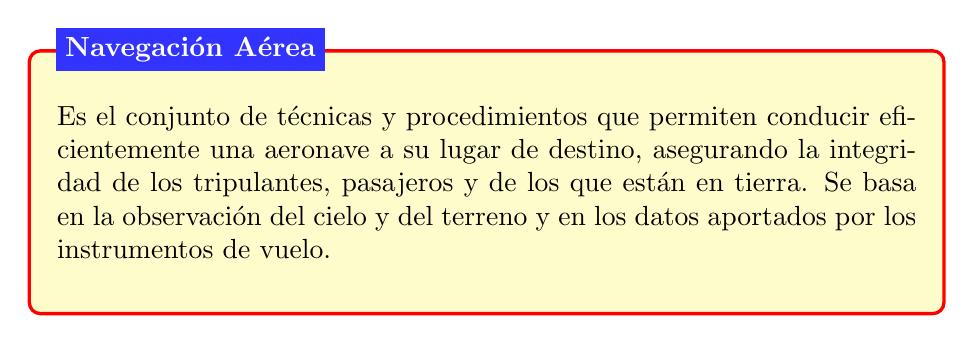
\begin{tikzpicture}
    \node [mybox] (box){%
      \begin{minipage}{0.90\textwidth}
	Es el conjunto de t\'ecnicas y procedimientos que permiten
        conducir eficientemente una aeronave a su lugar de destino,
        asegurando la integridad de los tripulantes, pasajeros y de
        los que est\'an en tierra. Se basa en la observaci\'on del
        cielo y del terreno y en los datos aportados por los
        instrumentos de vuelo.
      \end{minipage}
    }; \node[fancytitle, right=10pt] at (box.north west) {\bf Navegaci\'on
      A\'erea}; 
%\node[fancytitle, rounded corners] at (box.east){$\clubsuit$};
  \end{tikzpicture}%
\end{center}

\vspace{3mm}

% \colorbox{yellow!40}
% {\parbox{0.99\textwidth}
% {\bf 
% La navegaci\'on a\'erea es el conjunto de t\'ecnicas y procedimientos que permiten conducir eficientemente una aeronave a su lugar de destino, asegurando la integridad de los tripulantes y pasajeros y de los que est\'an en tierra. Se basa en la observaci\'on del cielo y el terreno y en los datos aportados por los instrumentos de vuelo.}
% }

Si bien durante mucho tiempo el t\'ermino navegaci\'on estuvo asociado esencialmente a barcos, el desarrollo de la aviaci\'on le agreg\'o una nueva dimensi\'on: adem\'as de la posici\'on horizontal (\gls{latitud} y \gls{longitud}), se necesita tambi\'en la altura de la aeronave para garantizar que no se acerca peligrosamente a alg\'un obst\'aculo. Se habla entonces de navegaci\'on 3D (\ac{3D}).

Finalmente, el gran congestionamiento del espacio a\'ereo en muchas partes del mundo hace necesario agregar otra variable m\'as: el tiempo. El tener disponible un sistema de navegaci\'on que permita mantener sincronizadas las operaciones de las aeronaves facilita el introducir m\'as aeronaves en el mismo espacio a\'ereo sin comprometer la seguridad. \'Esta es la navegaci\'on 4D, y est\'a siendo desarrollada actualmente. 

La navegaci\'on a\'erea se divide en dos tipos, dependiendo de si la aeronave es independiente o necesita de instalaciones exteriores a la aeronave para poder guiarse:

% \begin{multicols}{2}
%   \begin{itemize}
%   \item Navegaci\'on a\'erea aut\'onoma.
%   \item Navegaci\'on a\'erea no aut\'onoma.
%   \end{itemize}
% \end{multicols}


% La \textbf{navegaci\'on a\'erea aut\'onoma} es aquella que no necesita de alguna infraestructura o informaci\'on suministrada por un equipo exterior a la aeronave para poder completar con \'exito el vuelo. A su vez, \'esta se divide en:

% \begin{description}
%     \item [Navegaci\'on observada:] se basa en la observaci\'on directa por parte del navegante o piloto de las referencias necesarias en el terreno para conocer la posici\'on de la aeronave.
%     \item [Navegaci\'on a estima (Dead reckoning):] el navegante o piloto estima la posici\'on actual, conocidas la direcci\'on y la velocidad respecto al terreno.
%     \item [Navegaci\'on por fijaci\'on de la posici\'on:] \'esta a su vez se subdivide en navegaci\'on a\'erea astron\'omica, navegaci\'on a\'erea Doppler, navegaci\'on a\'erea inercial (INS = Inertial Navigation System).
% \end{description}

\begin{center}
  \begin{tikzpicture}
    \node [grupos] (box){%
      \begin{minipage}{0.90\textwidth}

	Es aquella que no necesita de alguna infraestructura o informaci\'on suministrada 
	por un equipo exterior a la aeronave para poder completar con \'exito el vuelo. 
	A su vez, \'esta se divide en:

\begin{description}
    \item [Navegaci\'on observada:] se basa en la observaci\'on directa por parte del navegante o piloto de las referencias necesarias en el terreno para conocer la posici\'on de la aeronave.
    \item [Navegaci\'on a estima (Dead reckoning):] el navegante o piloto estima la posici\'on actual, conocidas la direcci\'on y la velocidad respecto al terreno.
    \item [Navegaci\'on por fijaci\'on de la posici\'on:] \'esta a su vez se subdivide en navegaci\'on a\'erea astron\'omica, navegaci\'on a\'erea Doppler, navegaci\'on a\'erea inercial (INS = Inertial Navigation System).
\end{description}

    \end{minipage}
  }; \node[fancytitle.grupos] at (box.north) {\bf Navegaci\'on A\'erea Aut\'onoma};
\end{tikzpicture}
\end{center}

\begin{center}
  \begin{tikzpicture}
    \node [grupos] (box){%
      \begin{minipage}{0.90\textwidth}

 necesita de instalaciones exteriores para su guiado durante el vuelo, estas reciben el nombre de \emph{ayudas a la navegaci\'on}. Estas ayudas se pueden dividir a su vez dependiendo del tipo de informaci\'on que transmiten as\'i como del canal a trav\'es del cual lo hacen. As\'i, las ayudas pueden ser:

\begin{description}
    \item [Ayudas visuales al aterrizaje:] son instalaciones que proporcionan se\~nales visuales durante la etapa de aterrizaje de la aeronave.
    \item [Radioayudas:] Se basan en se\~nales radioel\'ectricas, usualmente generadas en instalaciones terrestres y recibidas a bordo.
    \item [Navegaci\'on por sat\'elite:] se basa en una constelaci\'on de sat\'elites que transmite rangos de se\~nales utilizados para el posicionamiento y localizaci\'on en cualquier parte del globo terrestre, ya sea en tierra, mar o aire. Estos permiten determinar las coordenadas geogr\'aficas y la altitud de un punto dado como resultado de la recepci\'on de se\~nales provenientes de dicha constelaci\'on.
\end{description}

    \end{minipage}
  }; 
\node[fancytitle.grupos] at (box.north) {\bf Navegaci\'on A\'erea No Aut\'onoma};
\end{tikzpicture}
\end{center}


\begin{figure}[!h]
  \centering
  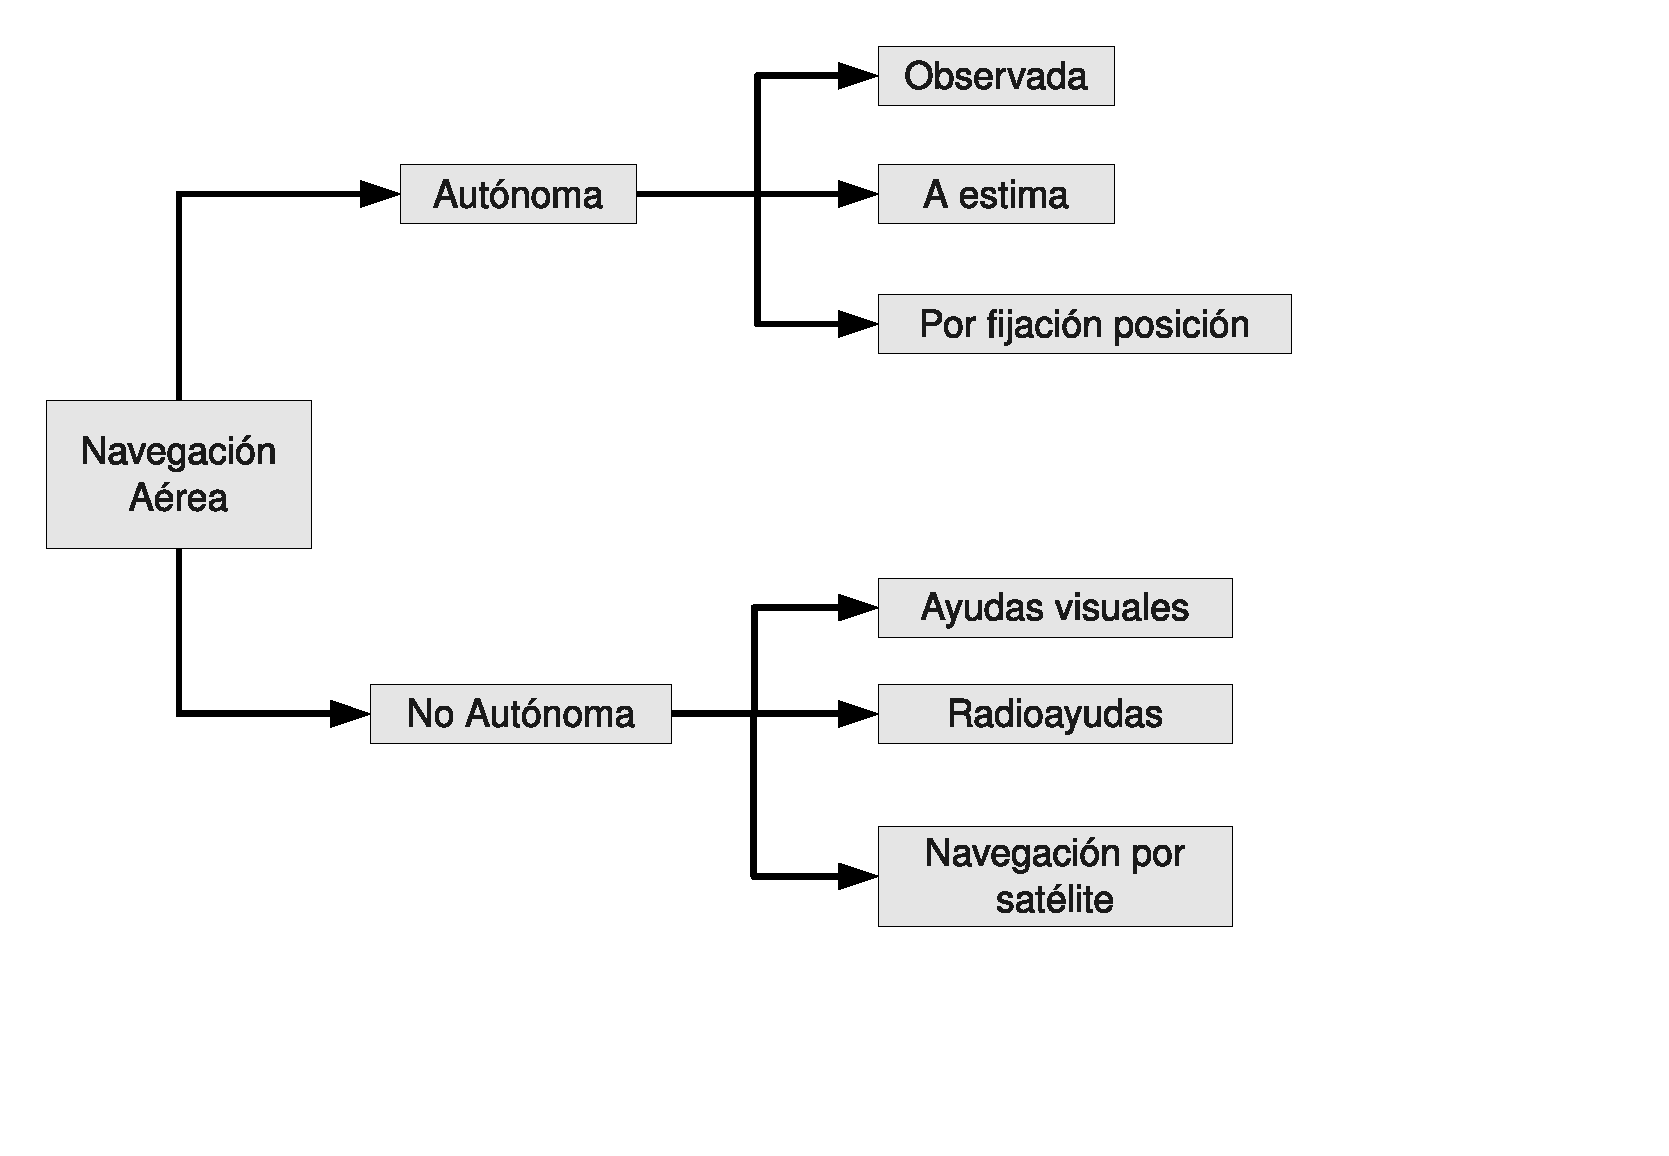
\includegraphics[width=\textwidth]{Imagenes/06.00.navegacion/tipos-navegacion.eps}
  \caption{Navegaci\'on A\'erea}
  \label{fig:navegacion.aerea.cuadro}
\end{figure}




\section{M\'etodos de Navegaci\'on A\'erea}

\subsection{Navegaci\'on Aut\'onoma}

\subsubsection{Navegaci\'on Observada \cite{Aena_SENASA_nav_aerea} }

 Es la que se realiza bas\'andose en
referencias del terreno que hay que ver, es una navegaci\'on visual.
Se trata de que el piloto localice las referencias del terreno, para lo
cual es fundamental el uso de buenos 
\begin{minipage}[b]{0.650\linewidth}
mapas en los que vengan
reflejados con claridad los accidentes geogr\'aficos, los pueblos y
ciudades, las carreteras y las v\'ias del ferrocarril, etc. \cite{Aena_SENASA_nav_aerea}

  Para este tipo de navegaci\'on se debe preparar el vuelo,
  estableciendo con toda precisi\'on la ruta que se va a seguir sobre
  el propio mapa.

  En el mismo mapa se marcan puntos en la ruta para dividirla por
  tramos, tratando de que las marcas coincidan con puntos de
  referencia de la ruta. Se deben calcular los tramos por kil\'ometros
  y tiempo que se tarda en volar de un punto a otro.

  Hay que tener buena informaci\'on meteorol\'ogica de toda la ruta y
  llevar la lista de las frecuencias de Torres y Centros de control.
  Si se encontrase perdido, basarse en la \'ultima posici\'on que se
  reconoci\'o y calcular la posici\'on probable por el tiempo
  transcurrido; en esa posici\'on probable tratar de reconocer alguna
  referencia significativa.

\end{minipage}
\begin{minipage}[b]{0.350\linewidth}
\centering
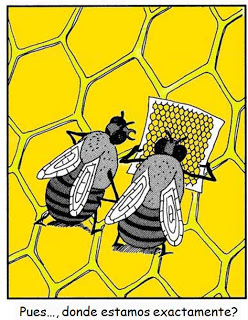
\includegraphics[width=0.9\textwidth]{Imagenes/06.00.navegacion/donde_estamos.jpg}  
\end{minipage}


%Establecer contacto por radio con la Torre o Centro de control m\'as apropiado y tratar de obtener marcaciones de radiogonometr\'ia pulsando el bot\'on del micr\'ofono de la radio, lo cual permitir\'ia al controlador dar una marcaci\'on QDM (rumbo a la estaci\'on), para llegar a alg\'un aeropuerto.



\subsubsection{Navegaci\'on a Estima (Dead Reckoning) \cite{Salazar_nav_aerea}}

  Dead reckoning es traducido en espa\~nol como ``\textit{navegacion
    por estima}'', es una expresi\'on derivada del t\'ermino n\'autico
  \textit{deduced reckoning} (c\'alculo basado en inferencia), y es un
  procedimiento matem\'atico que utiliza sencillas f\'ormulas
  trigonom\'etricas para inferir la ubicaci\'on actual de un nav\'io
  haciendo c\'alculos basados en el rumbo y la velocidad de
  navegaci\'on a lo largo de un per\'iodo de tiempo, sin usar el cielo
  y los astros como referencia.

  \begin{minipage}[b]{0.650\linewidth}
  

  La amplia mayor\'ia de sistemas de robots m\'oviles terrestres que
  se usan hoy en d\'ia, utilizan la t\'ecnica dead reckoning como
  columna vertebral de su estrategia de navegaci\'on, y al igual que
  sus hom\'ologos n\'auticos, necesitan eliminar los errores
  acumulados con continuos ajustes con varios sistemas de ayuda a la
  navegaci\'on.


  El principal problema que tiene la navegaci\'on a estima es que
  requiere la selecci\'on de una serie de puntos significativos de la
  ruta que tienen que estar
 a la vista de la tripulaci\'on, aunque en
  ocasiones estas referencias visuales no se obtienen, especialmente
  en vuelos nocturnos o con condiciones atmosf\'ericas adversas y en
  vuelos realizados sobre el mar.

\end{minipage}
\begin{minipage}[b]{0.35\linewidth}
    \centering
    
     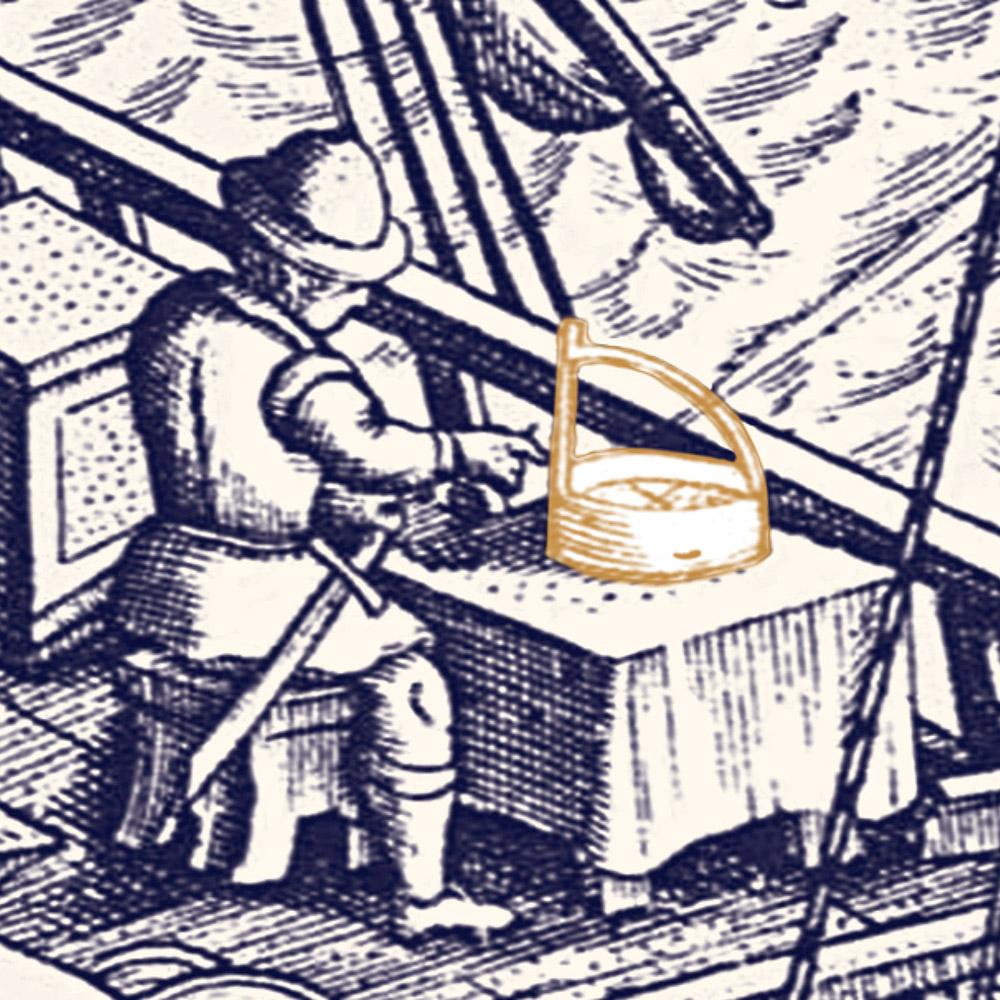
\includegraphics[width=0.90\textwidth]{Imagenes/06.00.navegacion/marinero-navegacion.jpg}
   \end{minipage}
%   \begin{minipage}[b]{0.50\linewidth}
% 	\centering
%   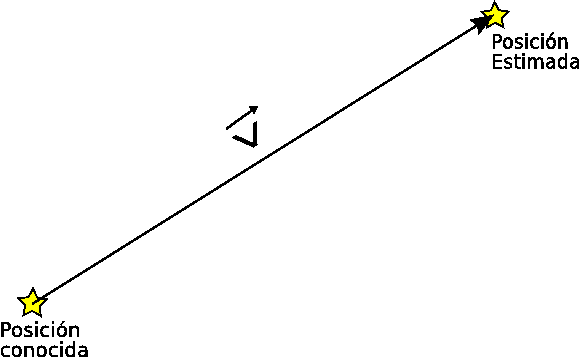
\includegraphics[keepaspectratio,width=0.9\textwidth]{./Imagenes/06.00.navegacion/dead-reckoning.png}
  
%   \end{minipage}
% %     \caption{Dead recokning en la navegaci\'on mar\'itima}
% % \label{fig:dead.reckoning.navegacion.maritima}
% % \end{figure}


  La implementaci\'on m\'as simple posible de la t\'ecnica dead
  reckoning es habitualmente llamada \emph{odometr\'ia}, t\'ermino que
  implica que el desplazamiento de un veh\'iculo a lo largo de la
  \gls{trayectoria} se deriva directamente de alg\'un od\'ometro o
  cuentarrevoluciones a bordo del veh\'iculo. Una t\'ecnica com\'un
  para implementar la odometr\'ia consiste en utilizar encoders
  \'opticos directamente acoplados a los motores o a los ejes de las
  ruedas.


\begin{figure}[!h]
  \centering
  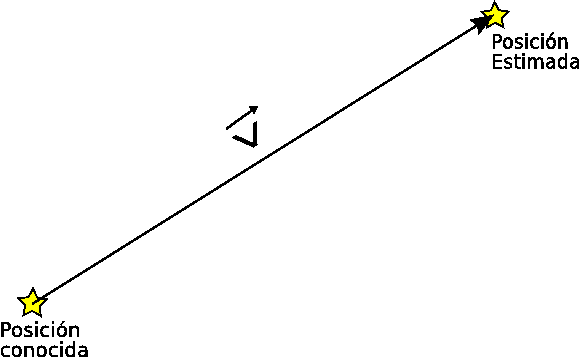
\includegraphics[keepaspectratio,width=0.7\textwidth]{./Imagenes/06.00.navegacion/dead-reckoning.png}
  \caption{Navegaci\'on a estima \cite{Salazar_nav_aerea}}
  \label{fig:dead-reckoning}
\end{figure}


Si, dado un marco de referencia arbitrario, las coordenadas de la posici\'on previa conocida $P_1$ son $(x_1, y_1)$ y las de la nueva posici\'on $P_2$ son $(x_2, y_2)$, entonces el vector que une ambas posiciones se puede denotar como $\vec x_{12}$, y en notaci\'on vectorial:


  \begin{equation}
\vec x_{12} = \vec x_2 - \vec x_1 = (x_2, y_2) - (x_1, y_1) = (x_2 - x_1, y_2 - y_1)
    \label{eq:dead-reckoning-vtor-posicion}
  \end{equation}



En forma matricial se expresar\'ia como:


\begin{equation}\label{eq:dead-reckoning-expresion-matricial}
 \vec x_{12} = \vec x_2 - \vec x_1 = 
\left\{ \begin{array}{c} x_2 \\ y_2 \end{array} \right\} 
- \left\{ \begin{array}{c} x_1 \\ y_1 \end{array} \right\} 
=
\left\{ \begin{array}{c} x_2 - x_1 \\ y_2 - y_1 \end{array} \right\}
\end{equation}

Y entonces, la navegaci\'on a estima implica que:

\begin{equation}
  \label{eq:dead-reckoning-otra-expresion}
\vec x_2 = \vec x_1 + \vec x_{12} = \vec x_1 + \int_{t_1}^{t_2} \vec v_{12} dt = \vec x_1 + \int_{t_1}^{t_2} \vec v dt   
\end{equation}

N\'otese que en la expresi\'on (\ref{eq:dead-reckoning-otra-expresion}) se asume que el vector $\vec x_{12}$ es igual a la integraci\'on del vector velocidad estimada $\vec v$. Esto no necesariamente es as\'i, debido a que el vector velocidad estimada $\vec v$ no necesariamente es igual al vector velocidad real $\vec v_{12}$. Esto en general se debe a:

\begin{minipage}[b]{0.70\linewidth}
  \begin{itemize}
  \item Una componente adicional a la velocidad del avi\'on, causada
    t\'ipicamente, por el viento ($v_w$). La acci\'on del viento, si
    no est\'a alineada con la velocidad del avi\'on, lo saca de su
    curso deseado (track).

  \item Por otra parte, si el viento est\'a alineado, pero en contra,
    causar\'a una sobre-estimaci\'on (overshoot) de la posici\'on (se
    estimar\'a que la aeronave est\'a m\'as all\'a de donde realmente
    est\'a), y si est\'a a favor causar\'a una sub-estimaci\'on
    (undershoot) de la posici\'on.

  \item Un error del sistema de navegaci\'on. Los errores m\'as
    perniciosos en este sentido son los \textbf{errores
      sistem\'aticos}, que son aquellos en los que hay un sesgo (o
    bias) que continuamente altera la medida en una misma direcci\'on
    (causando, por ejemplo, una desviaci\'on constante hacia la
    derecha de 0.1º por minuto).

  \end{itemize}
\end{minipage}
\begin{minipage}[b]{0.30\linewidth} \centering
  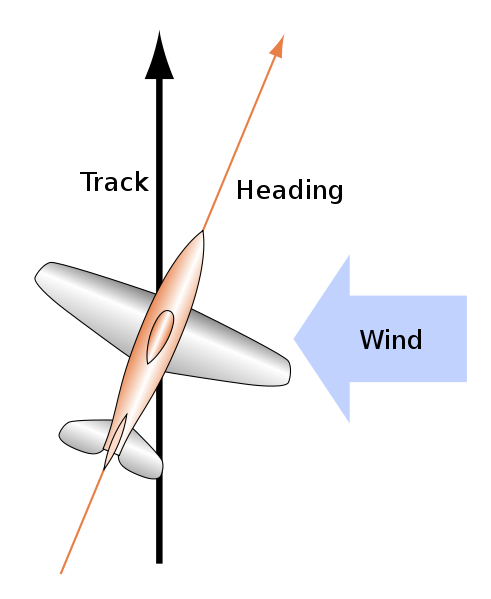
\includegraphics[width=0.85\textwidth]{Imagenes/06.00.navegacion/ajuste-viento.png}
	\captionof{figure}{El efecto del viento}
\end{minipage}

\begin{figure}[!h]
  \centering
  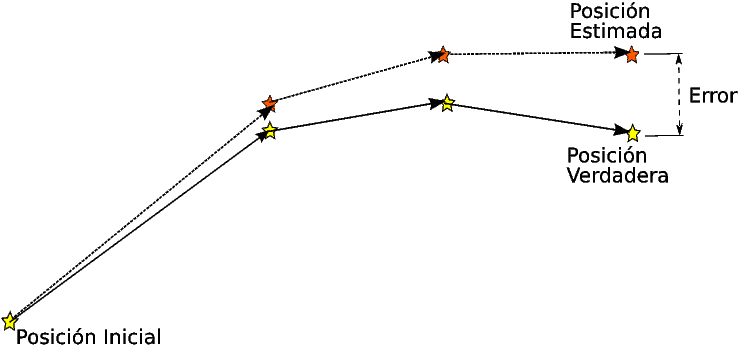
\includegraphics[keepaspectratio,width=0.8\textwidth]{./Imagenes/06.00.navegacion/dead-reckoning-error.png}  
  \caption{Error acumulativo en la navegaci\'on a estima \cite{Salazar_nav_aerea}}
  \label{fig:dead-reckoning-error}
\end{figure}

      
Debido al proceso de integraci\'on impl\'icito en este tipo de navegaci\'on, se tiene el inconveniente de que \textbf{los errores son acumulativos}, es decir, una peque\~na desviaci\'on en las estimaciones iniciales de la posici\'on se va convirtiendo con el paso del tiempo en un gran error, tal y como indica la Figura \ref{fig:dead-reckoning-error}.


Es por esta raz\'on que la navegaci\'on a estima debe combinarse con otros tipos de navegaci\'on (el visual, por ejemplo) para obtener una correcci\'on de la posici\'on que permita empezar una iteraci\'on ``\textit{fresca}'' del m\'etodo (es decir, cada cierto tiempo hace falta obtener un correcci\'on confiable).

Tambi\'en es conveniente acotar que la navegaci\'on a estima en aeron\'autica se usa para conocer la posici\'on en 2D.


\subsubsection{Navegaci\'on por Fijaci\'on de la Posici\'on}

%Se habla de navegaci\'on aut\'onoma cuando \'esta se realiza sin necesidad de utilizar se\~nales emitidas por transmisores de referencia en la tierra o en el espacio. Al principio se requiere partir de una posici\'on conocida y en la pr\'actica es necesario cotejar los resultados cada cierto tiempo usando otro tipo de navegaci\'on.


\begin{description}


\item[Navegaci\'on A\'erea Astron\'omica:] hace uso de la astronom\'ia para el uso directo del navegante a\'ereo, que comprende principalmente las coordenadas celestes, el tiempo y la posici\'on y movimiento aparente de los astros con respecto a la Tierra.

  \begin{minipage}[b]{0.60\linewidth}
    Se emplea en vuelos de larga distancia donde se carece de radio
    ayudas convenientes. Para utilizarla se requiere disponer de
    sextante, cron\'ometro, almanaque a\'ereo y tabla de
    reducci\'on. La combinaci\'on de los diferentes m\'etodos de
    navegaci\'on permite resolver el problema de navegaci\'on con
    mayor facilidad.

Con la evoluci\'on y desarrollo de las aeronaves, as\'i como el aumento de la autonom\'ia de vuelo, se hizo patente la necesidad de nuevos sistemas de posicionamiento que permitieran atravesar  zonas en las cuales las radio ayudas
  \end{minipage}
  \begin{minipage}[b]{0.40\linewidth} \centering
    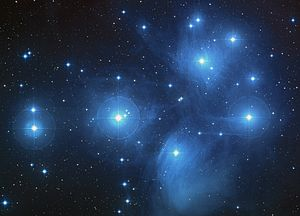
\includegraphics[width=0.85\textwidth]{Imagenes/06.00.navegacion/pleyades}
	\captionof{figure}{Las Pl\'eyades}
  \end{minipage}
 existentes no llegaban (por ejemplo en el mar). Para superar este problema se ech\'o mano de la navegaci\'on mar\'itima, la cual dispon\'ia desde muy antiguo de una t\'ecnica para establecer la posici\'on de un punto a partir de la observaci\'on de los astros. Para ello se utilizaban instrumentos tales como el astrolabio y el sextante. El Astrolabio permite localizar las posiciones de las estrellas sobre la b\'oveda celeste y se utilizaba para determinar la altura, la posici\'on y el movimiento de los astros sobre el horizonte. Este instrumento, tan antiguo y complejo, tiene adem\'as otro tipo de aplicaciones, como son: determinar la hora del d\'ia o de la noche, mediante la observaci\'on del Sol o de un Astro sobre el horizonte; calcular la hora de salida de las estrellas; as\'i como resolver problemas astrol\'ogicos m\'as complejos. 

 % \begin{figure}[!h]
 %   \centering
 %   \subfigure[Astrolabio]{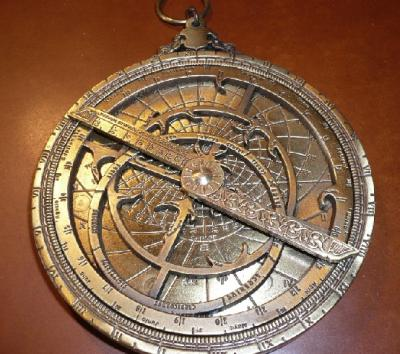
\includegraphics[height=6cm]{Imagenes/06.00.navegacion/astrolabio.jpg}}
 %   \subfigure[Sextante]{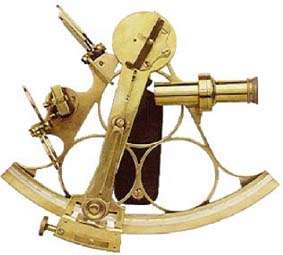
\includegraphics[height=6cm]{Imagenes/06.00.navegacion/sextante.jpg}   
 %   \caption{Instrumentos para navegaci\'on mar\'itima}
 %   \label{fig:instrumentos.navegacion.maritima}
 % \end{figure}

Poco tiempo despu\'es se invent\'o el sextante, que se basa en los mismos principios que el astrolabio pero se vale de dos nuevos elementos: un largavistas y un juego de espejos, cuyo uso de precisi\'on resultaron efectivos despu\'es de los estudios sobre \'optica. El sextante es un instrumento que permite medir \'angulos entre dos objetos tales como dos puntos de una costa o un astro -tradicionalmente el Sol- y el horizonte. Conociendo la elevaci\'on del Sol y la hora del d\'ia se puede determinar la latitud a la que se encuentra el observador. Esta determinaci\'on se efect\'ua con bastante precisi\'on mediante c\'alculos matem\'aticos sencillos de aplicar.

La navegaci\'on astron\'omica jug\'o un papel de complemento para la navegaci\'on a estima y sirvi\'o b\'asicamente para determinar la posici\'on cuando no era posible establecer referencias visuales con el terreno. Esta t\'ecnica de realizar peri\'odicamente la fijaci\'on de la posici\'on permiti\'o las m\'as importantes proezas registradas en el progreso de la aviaci\'on.

Por otra parte, los c\'alculos a realizar, a\'un con la utilizaci\'on de unos m\'etodos muy elaborados, exig\'ian una dedicaci\'on que no era compatible con la atenci\'on que la tripulaci\'on hab\'ia de destinar al control de la aeronave en vuelo. Esta situaci\'on supuso la aparici\'on del navegante como miembro adicional de la tripulaci\'on, capaz de establecer varias veces la posici\'on del avi\'on bas\'andose en la observaci\'on con sextante, de determinados cuerpos celestes y el empleo de almanaques que indicaban su posici\'on en las diferentes \'epocas del a\~no.




\item[Navegaci\'on A\'erea Doppler:] es un sistema de radar, el cual suministra a la tripulaci\'on, con alto grado de precisi\'on, la velocidad y el \'angulo de desviaci\'on (deriva) durante el vuelo a la vez que suministra datos visuales (lecturas) en millas n\'auticas, que lo separan del destino y millas que lo alejan a la izquierda o a la derecha del curso preseleccionado.

El sistema opera continua y autom\'aticamente sin la ayuda de estaciones de tierra. Fue dise\~nado utilizando el \textbf{Efecto Doppler}\footnote{ El \textbf{Efecto Doppler} es llamado as\'i por el austr\'iaco Christian Doppler consiste en la variaci\'on de la longitud de onda de cualquier tipo de onda emitida o recibida por un objeto en movimiento. Doppler propuso este efecto en 1842 en una monograf\'ia titulada Über das farbige Licht der Doppelsterne und einige andere Gestirne des Himmels (``Sobre el color de la luz en estrellas binarias y otros astros''). } ; recordando el mismo principio f\'isico de comportamiento de un objeto que se aproxima y se aleja: ``Que la frecuencia de una se\~nal observada a un punto fijo en el espacio es mayor que la observada en una fuente de se\~nal, si la fuente est\'a en movimiento hacia el punto fijo.''     Rec\'iprocamente, la frecuencia en el punto fijo ser\'a menor entonces que en la fuente, si la fuente se est\'a moviendo lejos del punto fijo.

Este aumento o disminuci\'on en frecuencia es proporcional a la velocidad a la cual la fuente de se\~nal se est\'a moviendo y si \'esta es constantemente monitoreada y medida por algunos m\'edios de precisi\'on, la informaci\'on obtenida puede ser usada para determinar el curso y la velocidad de la misma fuente de se\~nal.

En este caso, la fuente de se\~nal en el avi\'on es el mismo sistema DOPPLER y es este sistema igualmente el que constantemente monitorea y mide la se\~nal, la cual es reflejada en la superficie terrestre.

Usualmente se instalan dos sistemas en un avi\'on y consiste de una antena (usada para ambos sistemas), un TRANSCEPTOR (transmisor - receptor), una unidad seguidora (Tracker), un panel de control, un computador (no como lo conocemos actualmente), un controlador del computador y un indicador.

Cada sistema recibe informaci\'on de rumbo de uno de los dos sistemas de comp\'as y suministra al sistema de piloto autom\'atico informaci\'on de cualquiera de los sistemas DOPPLER.

Ambos sistemas operan simult\'aneamente y separadamente aunque reciben se\~nales de informaci\'on de una antena com\'un.



\item[Navegaci\'on A\'erea Inercial \cite{Salazar_nav_aerea}:] consiste en una plataforma estabilizada con gir\'oscopos que sirve como marco de referencia. En la misma unos aceler\'ometros y gir\'oscopos permiten medir los cambios de velocidad (tanto traslacional como rotacional) y, mediante integraci\'on sucesiva de los datos, obtener la posici\'on de la aeronave y su \gls{actitud}.
% , como se indica en las siguientes expresiones:


% \[
%  \begin{array}{l} \vec v(t) - \vec v_0 = \displaystyle \int_{t_0}^{t} \vec ... ...\\ \vec x(t) - \vec x_0 = \displaystyle \int_{t_0}^{t} \vec v dt \end{array}
% \]


% \[
%  \begin{array}{l} \vec \omega(t) - \vec \omega_0 = \displaystyle \int_{t_0}... ...(t) - \vec \theta_0 = \displaystyle \int_{t_0}^{t} \vec \omega dt \end{array}
% \]

% Donde:

%     * $\vec a$: Vector aceleraci\'on traslacional.

%     * $\vec v$: Vector velocidad traslacional.

%     * $\vec v$: Vector posici\'on.

%     * $\vec \alpha$: Vector aceleraci\'on angular.

%     * $\vec \omega$: Vector velocidad angular.

%     * $\vec \theta$: Vector posici\'on angular.

%Notese que, seg\'un las expresiones anteriores, 

En realidad se est\'a llevando a cabo un sofisticado proceso de dead reckoning  y que, debido a que la plataforma giro-estabilizada no es perfecta, en los c\'alculos se van introduciendo errores acumulativos que deben ser corregidos mediante fuentes externas al cabo de un cierto tiempo de vuelo.

Dicho tiempo es variable seg\'un la calidad del INS utilizado, un sistema de buena calidad acumula un error en distancia de un kil\'ometro o menos por hora, y el error angular t\'ipicamente es menor a pocas d\'ecimas de grado por hora. 

\end{description}

\subsection{Navegaci\'on A\'erea No Aut\'onoma}

\subsubsection{Ayudas visuales}

Utilizadas casi desde los inicios mismos de la aviaci\'on, por lo general est\'an asociadas a la operaci\'on de aterrizaje:
\begin{description}
\item [De punto fijo] Permiten identificar f\'acilmente desde lo lejos un punto de referencia importante. El faro aeron\'autico es el ejemplo t\'ipico.

    \item [De direcci\'on] Proporcionan al piloto informaci\'on valiosa sobre la direcci\'on de, por ejemplo, el viento (manga de viento) o el eje de la pista (luces de eje de pista).

    \item [De elevaci\'on] En este caso se indica al piloto el \'angulo vertical con el que se aproxima a la pista. Entran en esta categor\'ia los sistemas de luces PAPI (ver Figura \ref{fig:papi}), VASI, etc.

\end{description}
     

En la Figura \ref{fig:papi} se muestra el t\'ipico emplazamiento de un sistema PAPI. 



\subsubsection{Radioayudas}

Las radioayudas se pueden clasificar seg\'un el tipo de informaci\'on que proporcionan:

\begin{description}
\item [Direcci\'on a un punto fijo] Este tipo de ayudas simplemente indica, mediante una aguja, la direcci\'on en la que tendr\'ia que volar el piloto para llegar a un punto de referencia dado. A este tipo pertenece el sistema ADF/NDB.

    \item [Azimutales] El azimut es el \'angulo horizontal formado entre un eje de referencia (por ejemplo el vector radioayuda norte magn\'etico), y el vector radioayuda aeronave. En esta clasificaci\'on entran, entre otros, el VOR y el ILS/LLZ.
      Usar una radioayuda azimutal a menudo se de\-no\-mi\-na navegaci\'on theta ($\theta$), por la notaci\'on que recibe habitualmente el \'angulo proporcionado (azimut).

    \item [Cenitales] En este caso se proporciona el \'angulo vertical entre el eje de referencia radioayuda-horizonte y el vector radioayuda-aeronave. El ILS/GS es el ejemplo t\'ipico.

    \item [De distancia] Este tipo de ayudas proporcionan la distancia entre radioayuda y aeronave. Como esta distancia a menudo se denota como ``rho'' ($\rho$), se habla entonces de navegaci\'on rho. A esta categor\'ia pertenece el DME.

\end{description}
     
En la Figura \ref{fig:DVOR-vista-aerea} se presenta la vista a\'erea de una estaci\'on VOR en B\'elgica. 



\begin{figure}[!h]
  \centering

\subfigure[Precision Approach Path Indicator - PAPI \cite{wikipedia_esp} ]{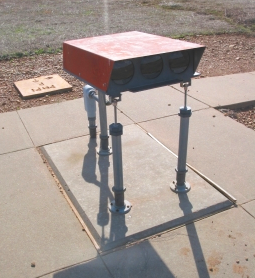
\includegraphics[keepaspectratio,height=7cm]{./Imagenes/06.00.navegacion/papi.png}
  \label{fig:papi}}
\subfigure[Vista a\'erea de un VOR \cite{wikipedia_esp}]{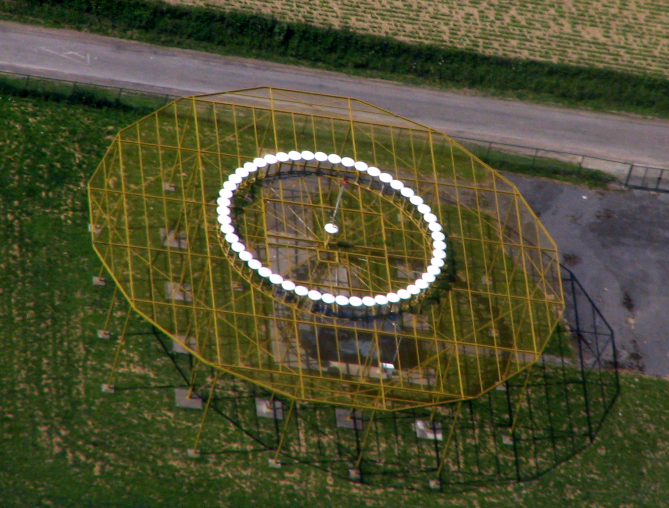
\includegraphics[keepaspectratio,height=7cm]{./Imagenes/06.00.navegacion/DVOR-aerea.png}
  \label{fig:DVOR-vista-aerea}}

\caption{Ayudas visuales}
\end{figure}




\subsubsection{Navegaci\'on por sat\'elite}

Los \'ultimos avances en la tecnolog\'ia espacial est\'an generando una revoluci\'on en la manera como se realiza la navegaci\'on. De hecho, se estima que antes del 2020 los sistemas basados en navegaci\'on por sat\'elite sustituir\'an a casi todos los dem\'as sistemas utilizados actualmente.

Estos sistemas reciben el nombre gen\'erico de GNSS (Global Navigation Satellite Systems) porque su cobertura es mundial. Los representantes m\'as importantes son:

\begin{description}
\item [GPS] Sistema estadounidense de origen militar, es actualmente el m\'as conocido y desarrollado. Empez\'o a operar a principios de la d\'ecada de 1980 y se est\'an ejecutando planes para su modernizaci\'on.% La Figura \ref{fig:satelite-GPS} es una representaci\'on art\'istica de un sat\'elite GPS de la generaci\'on IIF.
 En 1957 la Uni\'on Sovi\'etica lanz\'o al espacio el sat\'elite Sputnik I, que era monitorizado mediante la observaci\'on del Efecto Doppler de la se\~nal que transmit\'ia. Debido a este hecho, se comenz\'o a pensar que, de igual modo, la posici\'on de un observador podr\'ia ser establecida mediante el estudio de la frecuencia Doppler de una se\~nal transmitida por un sat\'elite cuya \'orbita estuviera determinada con precisi\'on.
La Armada estadounidense r\'apidamente aplic\'o esta tecnolog\'ia, para proveer a los sistemas de navegaci\'on de sus flotas de observaciones de posiciones actualizadas y precisas. As\'i surgi\'o el sistema TRANSIT, que qued\'o operativo en 1964, y hacia 1967 estuvo disponible, adem\'as, para uso comercial.
Las actualizaciones de posici\'on, en ese entonces, se encontraban disponibles cada 40 minutos y el observador deb\'ia permanecer casi est\'atico para poder obtener informaci\'on adecuada.
Posteriormente, en esa misma d\'ecada y gracias al desarrollo de los relojes at\'omicos, se dise\~n\'o una constelaci\'on de sat\'elites, portando cada uno de ellos uno de estos relojes y estando todos sincronizados con base en una referencia de tiempo determinada.
En 1973 se combinaron los programas de la Armada y el de la Fuerza A\'erea de los Estados Unidos (este \'ultimo consistente en una t\'ecnica de transmisi\'on codificada que prove\'ia datos precisos usando una se\~nal modulada con un c\'odigo de ruido pseudo-aleatorio (PRN = Pseudo-Random Noise), en lo que se conoci\'o como Navigation Technology Program, posteriormente renombrado como NAVSTAR GPS.
Entre 1978 y 1985 se desarrollaron y lanzaron once sat\'elites prototipo experimentales NAVSTAR, a los que siguieron otras generaciones de sat\'elites, hasta completar la constelaci\'on actual, a la que se declar\'o con «capacidad operacional inicial» en diciembre de 1993 y con «capacidad operacional total» en abril de 1995.
En 1994, este pa\'is ofreci\'o el servicio normalizado de determinaci\'on de la posici\'on para apoyar las necesidades de la OACI, y esta acept\'o el ofrecimiento.

    \item [GLONASS] La respuesta sovi\'etica al GPS, con las dificultades econ\'omicas de la ex-URSS cay\'o a niveles de inoperatividad. Sin embargo, hay planes de reactivarlo gracias a la ayuda de la Uni\'on Europea.

Los tres primeros satelites fueron colocados en \'orbita en octubre de 1982. El sistema fue pensado para ser funcional en el a\~no 1991, pero la constelaci\'on no fue terminada hasta diciembre de 1995 y comenz\'o a ser operativo el 18 de enero de 1996. Ese mismo a\~no la ya Federaci\'on Rusa ofreci\'o el canal de exactitud normalizada (CSA) del GLONASS para apoyar las necesidades de la OACI, y \'esta acept\'o el ofrecimiento.

La situaci\'on econ\'omica de Rusia a partir de 1990 supuso que en abril de 2002 s\'olo 8 sat\'elites estuvieran completamente operativos.

En el 2004, 11 sat\'elites se encontraban en pleno funcionamiento. A fines de 2007 son 19 los sat\'elites operativos. Son necesarios 18 satelites para dar servicio a todo el territorio ruso y 24 para poder estar disponible el sistema en todo el mundo.

En 2007, Rusia anunci\'o que a partir de ese a\~no se eliminan todas las restricciones de precisi\'on en el uso de GLONASS, permitiendo as\'i un uso comercial ilimitado. Hasta ahora las restricciones de precisi\'on para usos civiles eran de 30 m.

La aparici\'on en el mercado de receptores que permiten recibir se\~nales pertenecientes a los dos sistemas GLONASS y GPS (con sistemas de referencia diferentes) hace interesante las posibilidades de GLONASS en la medici\'on como apoyo al GPS norteamericano.

    \item [GALILEO] Es el futuro sistema GNSS, totalmente civil, actualmente en desarrollo por parte de la Uni\'on Europea. Poseer\'a caracter\'isticas que lo har\'an mucho m\'as avanzado que el GPS. Inicialmente Galileo iba a estar disponible en el 2008 aunque el proyecto acumula ya tres a\~nos de retraso y no podr\'a comercializar sus primeros servicios hasta 2011, entre temores de que esa fecha pueda demorarse hasta 2014, entre otros motivos, por disensiones entre los pa\'ises participantes.

El 28 de diciembre de 2005 se lanz\'o el sat\'elite Giove-A (Galileo in-orbit validation element), primero de este sistema de localizaci\'on por sat\'elite, desde el cosm\'odromo de Baikonur, en Kazajist\'an. El segundo de los sat\'elites de prueba, el Giove-B deber\'ia haberse lanzado en abril de 2006, pero por problemas con el ordenador a bordo, el lanzamiento fue retrasado hasta el pasado 25 de abril de 2008, teniendo lugar desde el mismo cosm\'odromo.

En abril de 2004 entr\'o en funcionamiento el sistema EGNOS, un sistema de apoyo al GPS para mejorar la precisi\'on de las localizaciones. En otras regiones del mundo hay otros sistemas similares compatibles con EGNOS: WAAS de Estados Unidos, MSAS de Jap\'on y el GAGAN de la India.

Las fases establecidas para la implementaci\'on del sistema son:

\begin{itemize}
\item Definici\'on (2000-2003)
    \item Desarrollo y validaci\'on en \'orbita (2004-2008)
    \item Despliegue (2008-2010)
    \item Explotaci\'on comercial (a partir de 2010 - 2015)
\end{itemize}

La Rep\'ublica Popular China (RPC) es, desde el 9 de octubre de 2004, el primer pa\'is no europeo que participa en el programa Galileo, tras la firma del acuerdo en Pek\'in por la, en ese momento, vicepresidenta de la Comisi\'on Europea, Loyola de Palacio.

China aportar\'a 200 millones de euros del total de 3.200 millones del proyecto pese a las reticencias de algunos miembros europeos por transferir tecnolog\'ia a China. En julio de 2005 la UE firm\'o contratos con varias compa\~n\'ias chinas para desarrollar aplicaciones comerciales para Galileo.

Se ha firmado ya un acuerdo con Israel y con India (septiembre de 2005), y se est\'a en conversaciones con Brasil, Jap\'on, Corea del Sur, Australia y Ucrania.

\end{description}
     
\begin{figure}[!h]
  \centering
  \subfigure[Sat\'elite GPS generaci\'on IIF \cite{wikipedia_esp}]{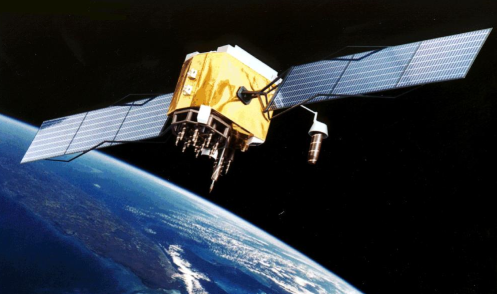
\includegraphics[keepaspectratio,height=5cm]{./Imagenes/06.00.navegacion/GPS-Satellite-IIF.png}
  \label{fig:satelite-GPS}}
  \subfigure[Sat\'elite GLONASS]{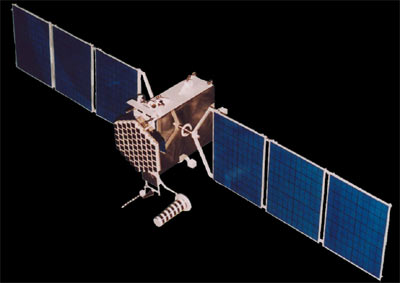
\includegraphics[keepaspectratio,height=5cm]{./Imagenes/06.00.navegacion/glonass.jpg}
  \label{fig:satelite-GPS}}
  \subfigure[Sat\'elite GALILEO]{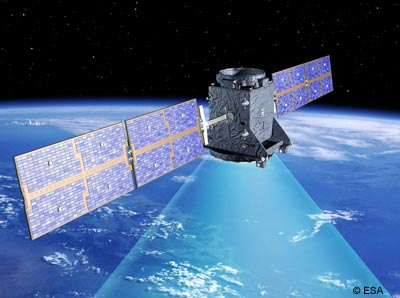
\includegraphics[keepaspectratio,height=5cm]{./Imagenes/06.00.navegacion/gps-galileo.jpg}
  \label{fig:satelite-GPS}}
  \caption{Navegaci\'on por sat\'elite}
\end{figure}

Es muy importante acotar que en la actualidad ninguno de los sistemas GNSS operativos pueden utilizarse, por s\'i solo, como m\'etodo \'unico de navegaci\'on a\'erea. Hay varias causas para esto:

\begin{itemize}
\item  Tanto el sistema GPS como el GLONASS son de
  naturaleza militar y no hay garant\'ia de que operen continuamente
  para los usuarios civiles (GALILEO se encuentra aun en fase de
  desarrollo).

\item  Ninguno de los sistemas GNSS proporciona,  actualmente, integridad. Es decir, la garant\'ia de que el piloto
  recibir\'a r\'apidamente y de manera autom\'atica la advertencia de que el
  sistema tiene una falla y dej\'o de funcionar adecuadamente.

\item  No hay garantia o cobertura de fiabilidad prove\'ida por sus operadores (e.g. accidentes aereos)
\item La fiabilidad es incierta en regiones de altas latitudes del norte de Europa
\item La precisi\'on es moderada para aplicaciones que requieren una r\'apida determinaci\'on de la posici\'on
\item A los usuarios no se les informa inmediatamente de los errores que ocurren en el sistema
\end{itemize}

Es por esta raz\'on que se han desarrollado sistemas adicionales a los GNSS que los complementan. \'Estos son los llamados \textbf{Sistemas de Aumento} y existen b\'asicamente tres categor\'ias:


\begin{description}
\item [SBAS] Sistemas de aumento basados en sat\'elites. Proporcionan sat\'elites auxiliares y estaciones de referencia en tierra con funciones espec\'ificas que complementan a los GNSS y los hacen aptos
  para navegaci\'on en ruta y aproximaciones a la pista. Los ejemplos
  son WAAS (estadunidense), EGNOS (europeo) y MSAS (japon\'es).

\item [GBAS] Sistemas de aumento basados s\'olo en instalaciones en
  tierra. El ejemplo t\'ipico es el LAAS (a\'un en desarrollo), son de
  corto alcance y est\'an enfocados en la asistencia en el aterrizaje.

\item [ABAS] Sistemas de aumento basados en instrumentos a bordo de la
  aeronave. Combinan informaci\'on de varios instrumentos aeron\'auticos y
  en funci\'on de esto monitorizan el estado de los sat\'elites GNSS.
\end{description}


\section{M\'etodos para determinar la posici\'on \cite{Salazar_nav_aerea}}

Adicionalmente al m\'etodo dead reckoning,  existen varias maneras de obtener la posici\'on seg\'un la naturaleza de las ayudas de navegaci\'on disponibles para el aeronavegante. 


\subsection{M\'etodo $\theta-\theta$}

Este m\'etodo se utiliza cuando se tienen disponibles varias radioayudas de tipo azimutal, o en general, cuando el sistema de navegaci\'on obtiene \'angulos entre ejes de referencia, puntos de referencia y la posici\'on actual.

Para explicar los fundamentos del m\'etodo, se debe imaginar que el sistema de navegaci\'on de la aeronave obtiene el \'angulo $\theta_1$ entre la posici\'on de la aeronave, el punto de referencia $P_1$ y un eje de referencia, tal y como ilustra la Figura \ref{fig:theta-fix}. Si el punto de referencia es, por ejemplo, una estaci\'on VOR, el eje de referencia apunta al norte magn\'etico. 

El conocimiento del \'angulo $\theta_1$ determina una l\'inea de posici\'on (o LOP, por sus siglas en ingl\'es). Se sabe entonces que la aeronave se encuentra en alg\'un lugar a lo largo de $LOP_{1}$: la l\'inea que empieza en el punto $P_1$ y se aleja de dicho punto en la direcci\'on $\theta_1$.

Si se toma un marco de referencia rectangular de origen cualquiera, con su eje $Y$ paralelo al el eje de referencia hacia el norte de la radioayuda, y se supone que las coordenadas del punto $P_1$ en dicho sistema vienen dadas por $(x_1, y_1)$, entonces se tiene una situaci\'on como la mostrada en la Figura\ref{fig:theta-lop1}. 

\begin{figure}[!h]
  \centering
 \subfigure[M\'etodo $\theta$]{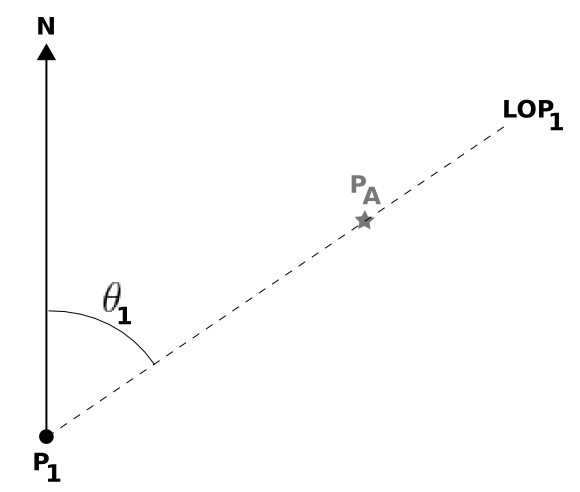
\includegraphics[width=0.45\textwidth]{./Imagenes/06.00.navegacion/theta-fix.png}  \label{fig:theta-fix}}
\subfigure[M\'etodo $\theta$ con marco de referencia ]{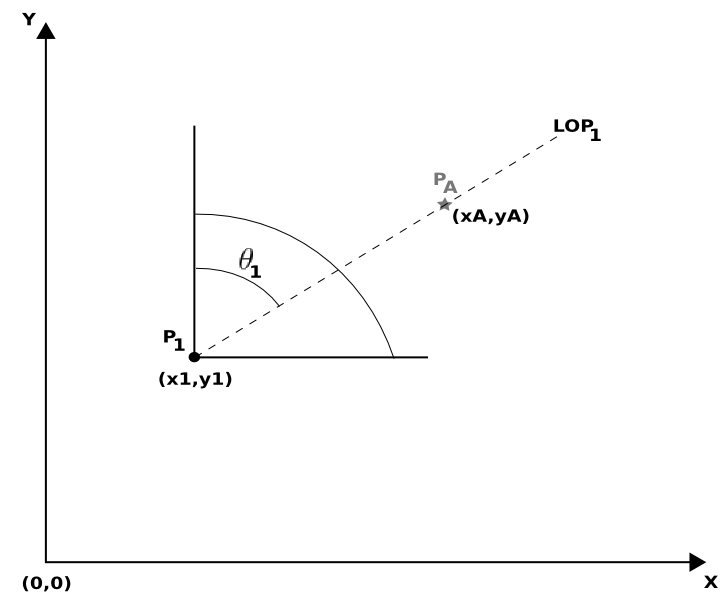
\includegraphics[width=0.45\textwidth]{./Imagenes/06.00.navegacion/theta-lop1.png}  \label{fig:theta-lop1}}
  \caption{M\'etodo $\theta-\theta$}
\end{figure}

Entonces, se puede demostrar que la posici\'on $(x_A, y_A)$ de la aeronave es posible expresarla de manera simple como la ecuaci\'on de una recta:


\begin{equation}\label{eq:metodo-theta}
 y_A = \tan (90-\theta_1) (x_A-x_1) + y_1
 \end{equation}





Sin embargo esta informaci\'on, aunque muy \'util, es insuficiente para determinar la posici\'on exacta de la aeronave: existe un n\'umero infinito de posiciones que cumple con la condici\'on establecida por la $LOP_{1}$ (Ecuaci\'on \ref{eq:metodo-theta}). Est\'a claro que se tiene una \'unica ecuaci\'on y que existen dos inc\'ognitas

Es por ello que se dice que hay una ambigüedad en la posici\'on. Para resolverla, es necesario obtener informaci\'on adicional. Hablando en t\'erminos matem\'aticos, es necesario encontrar otra ecuaci\'on que no sea linealmente dependiente de la primera.

Ahora bien, si dentro del alcance del sistema de navegaci\'on de la aeronave se encuentra otra estaci\'on VOR $P_2$ que proporcione una segunda medici\'on $\theta_2$, la situaci\'on ser\'a la planteada en la Figura \ref{fig:Theta-theta-fix}.

\begin{figure}[!h]
  \centering
  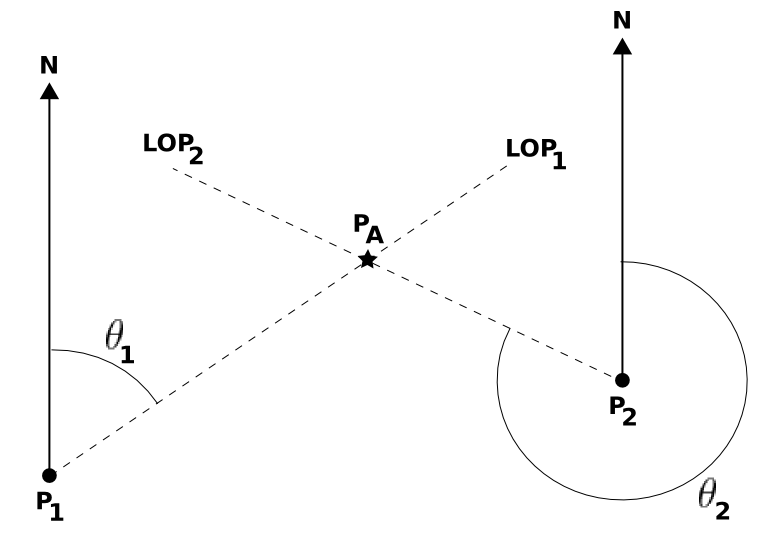
\includegraphics[width=0.5\textwidth]{./Imagenes/06.00.navegacion/theta-theta-fix.png}
  \caption{Theta-theta fix}
  \label{fig:Theta-theta-fix}
\end{figure}

En este caso, se tiene una segunda l\'inea de posici\'on $LOP_2$, que al intersectarse con $LOP_1$ proporcionar\'a la posici\'on de la aeronave. La Ecuaci\'on (\ref  {eq:theta-theta-fix}) representa a $LOP_2$.

\begin{equation}
  \label{eq:theta-theta-fix}
 y_A = \tan (90-\theta_2) (x_A-x_2) + y_2   
\end{equation}


Las Ecuaciones (\ref{eq:metodo-theta}) y (\ref  {eq:theta-theta-fix}) se combinan entonces para resolver el sistema y obtener la posici\'on.

Obviamente, en las consideraciones anteriores se ha supuesto que las coordenadas de los puntos $P_1$ y $P_2$ eran conocidas (de all\'i que se les considere puntos de referencia). Por lo general, esto supone que dichos puntos est\'an en lugares fijos. No obstante, pudiera darse el caso de que dichos puntos fueran m\'oviles, y entonces el sistema de navegaci\'on deber\'ia tener informaci\'on suficiente para calcular la posici\'on de los puntos de referencia en cada instante (como se hace, por ejemplo, con los sat\'elites de los sistemas GNSS). 

\subsection{M\'etodo $\theta-\rho$}

En ocasiones, junto con el VOR puede existir una estaci\'on DME colocalizada1.4 en el punto $P_1$. En este caso, adem\'as de un \'angulo $\theta_1$ se tiene una distancia o rango $\rho_1$, como indica la Figura \ref{fig:theta-rho-fix}.

\begin{figure}[!h]
  \centering
  \subfigure[M\'etodo $\theta-\rho$]{
     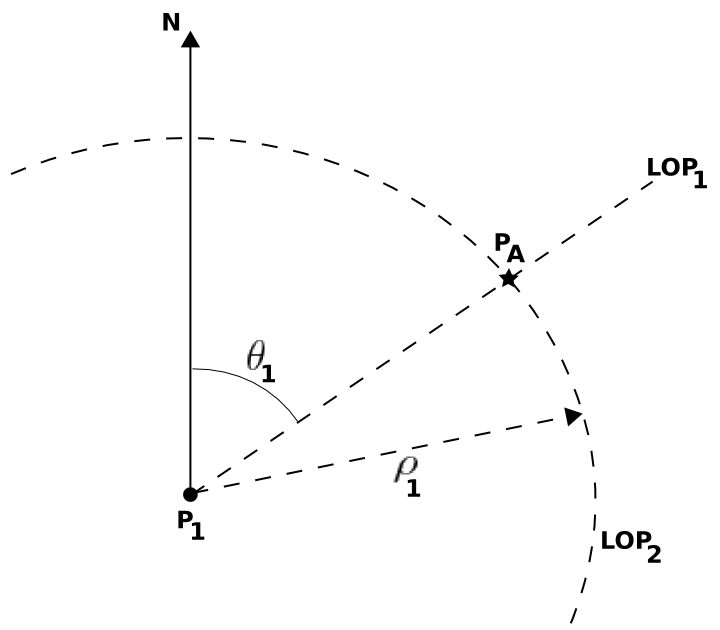
\includegraphics[height=6cm]{./Imagenes/06.00.navegacion/theta-rho-fix.png}  
     \label{fig:theta-rho-fix}
   }
  \subfigure[M\'etodo $\rho$-$\rho$]{
  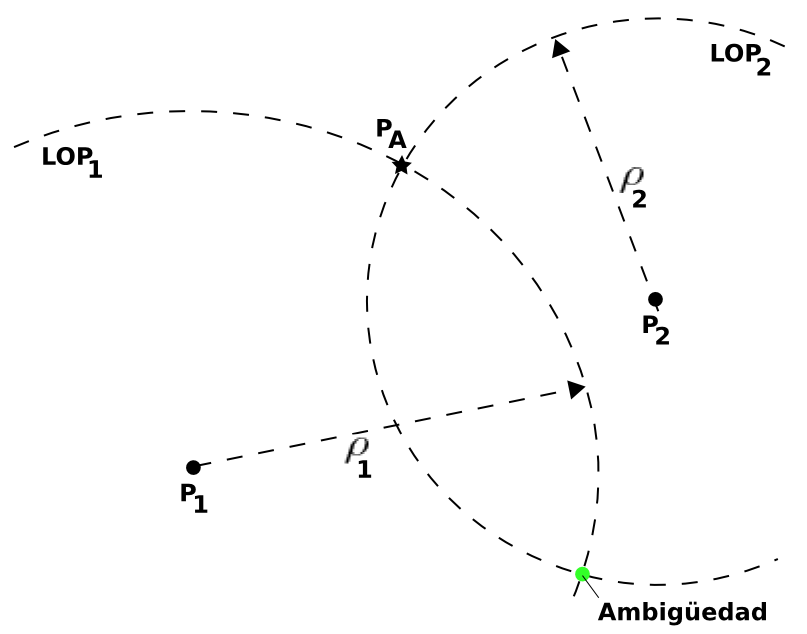
\includegraphics[height=6cm]{./Imagenes/06.00.navegacion/rho-rho-fix.png} 
  \label{fig:rho-rho-fix}
  }
  \caption{M\'etodos de navegaci\'on}
\end{figure}


Como puede verse, hay dos l\'ineas de posici\'on: $LOP_1$ correspondiente al \'angulo $\theta_1$ y $LOP_2$, que corresponde al rango $\rho_1$ (de hecho, est\'a ``\textit{l\'inea de posici\'on}'' es en realidad una circunferencia, pero el concepto se mantiene). En la intersecci\'on entre ambas LOPs se encuentra la aeronave.

La ecuaci\'on que corresponde a $LOP_2$ se puede expresar como:


\[ (y_A - y_1)^2 + (x_A - x_1)^2 = \rho_{1}^{2} \]

Note que este sistema puede resolverse incluso si el VOR y el DME no est\'an en el mismo lugar. Asimismo, es posible que la LOP de $\rho$ constante intersecte a la LOP de $\theta$ constante en m\'as de un lugar, dando como resultado una ambigüedad que deba resolverse con informaci\'on adicional. 


\subsection{M\'etodo $\rho$-$\rho$}

En este caso, se tienen al menos dos radioayudas que proporcionan informaci\'on de distancia, como se indica en la Figura \ref{fig:rho-rho-fix}

Se puede ver con facilidad la aparici\'on de una ambigüedad en la parte inferior de la Figura \ref{fig:rho-rho-fix}. Las fuentes de informaci\'on adicional usadas habitualmente para resolver dicha ambigüedad son:

\begin{itemize}\item  Agregar mediciones (ecuaciones) adicionales (de $\rho$ o $\theta$)
  que permitan discernir la posici\'on correcta.

\item Dado que la aeronave despega de una posici\'on conocida, un registro
  cuidadoso de la ruta seguida puede permitir discriminar cu\'al es la
  posici\'on correcta. Esto significa que se est\'a utilizando informaci\'on
  adicional del pasado (en vez del presente) para resolver la
  ambigüedad.

\item Para veh\'iculos terrestres y acu\'aticos, a veces es posible utilizar
  informaci\'on sobre el entorno para resolver la ambigüedad. Por
  ejemplo, el sistema de navegaci\'on de un barco puede descartar una
  ambigüedad que caiga en tierra, y el de un coche podr\'ia eliminar
  todas las posiciones posibles que caigan fuera de calles y
  carreteras.
\end{itemize}

\subsection{M\'etodo hiperb\'olico}

El m\'etodo hiperb\'olico es una versi\'on del $\rho$-$\rho$, pero en vez de utilizar los rangos absolutos se utiliza la diferencia entre ellos. Variaciones del m\'etodo usan la diferencia entre fases, o tiempos de recepci\'on, como muestran los diversos sistemas de navegaci\'on que utilizaban este m\'etodo, como el Omega, el LORAN, el Decca, etc.

El uso de la diferencia entre rangos genera LOPs que son hip\'erbolas, como muestra la Figura \ref{fig:metodo-hiperbolico}.

\begin{figure}[!h]
  \centering
  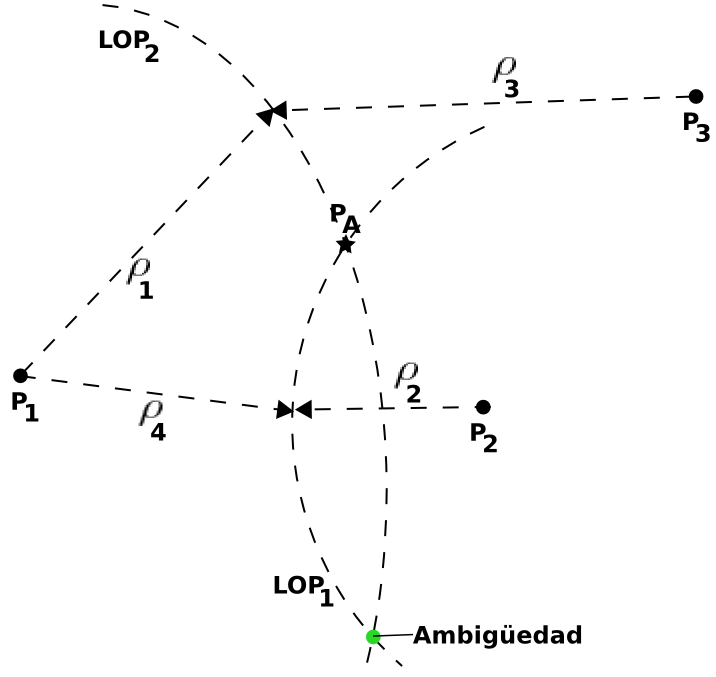
\includegraphics[width=0.5\textwidth]{./Imagenes/06.00.navegacion/hiperbolic-fix.png}
  \caption{M\'etodo hiperb\'olico}
  \label{fig:metodo-hiperbolico}
\end{figure}

Note que en la Figura  \ref{fig:metodo-hiperbolico} la ambigüedad queda resuelta al generar la hip\'erbola entre los puntos $P_2$ y $P_3$. 


\section{La Tierra}
\label{sec:la.tierra}

\subsection{Forma, tama\~no y movimientos}
\label{sec:forma.y.tamanio}

Desde el punto de la navegaci\'on, el planeta Tierra se considera una esfera perfecta, aunque en la realidad no lo sea. Inspecciones detalladas de su superficie han determinado variaciones en altura de, aproximadamente, 19 km desde el fondo del oc\'eano hasta el v\'ertice de la monta\~na m\'as alta, Figura \ref{fig:forma.tierra}.

Medida en el ecuador, el di\'ametro de la Tierra es aproximadamente $12756.274$\,km, mientras que el di\'ametro polar es de $12713.505$\,km. La diferencia entre estos di\'ametros es de $42.769$\,km y, este valor, puede ser utilizado para expresar la elipticidad de la Tierra (Figuras \ref{fig:dimensiones.tierra} y \ref{fig:amanecer.de.la.tierra}). El radio entre esta diferencia y el di\'ametro ecuatorial es:

\[\displaystyle
	\text{Elipticidad} = \frac{42.769 \,\text{m}}{ 12756.274\,\text{m}}
	=\frac{1}{298.257}
\]

\begin{figure}[!h]
  \centering

\subfigure[Forma de la tierra, dimensiones exageradas]{
	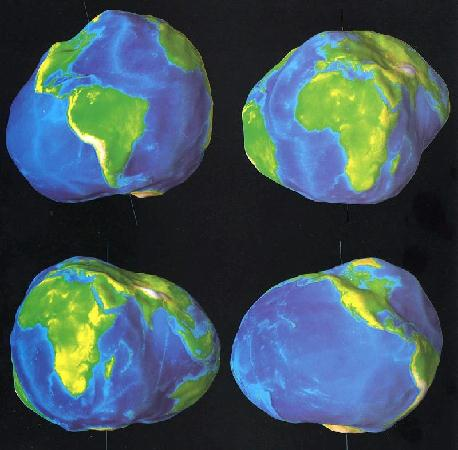
\includegraphics[height=6cm]{Imagenes/06.00.navegacion/forma-tierra.jpg}
	\label{fig:forma.tierra}}
  \subfigure[Amanecer de la Tierra, misi\'on \mbox{Apolo 8} (1968)]{
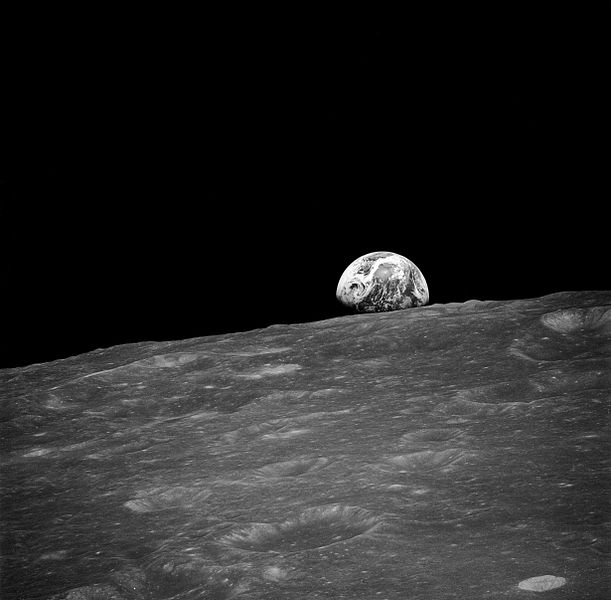
\includegraphics[height=6cm]{Imagenes/06.00.navegacion/amanecer-tierra.jpg}
 \label{fig:amanecer.de.la.tierra}}

  \subfigure[Dimensiones
%\\ {\tiny (Fuente: \url{http://www.kalipedia.com/geografia-general/tema/forma-dimensiones-tierra.html?x=20070417klpgeogra_6.Kes\&ap=1})}}
]{
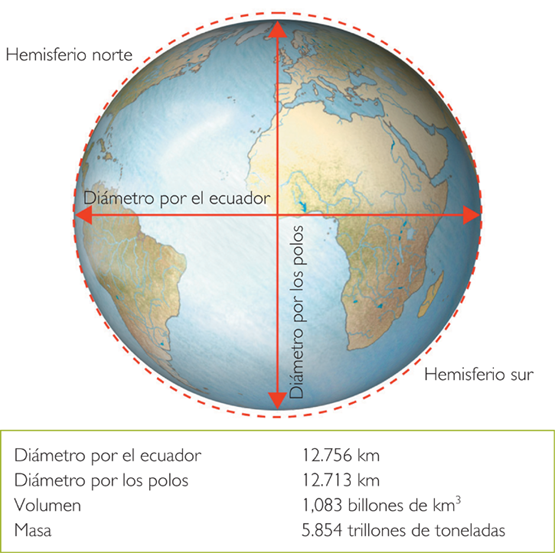
\includegraphics[height=6.5cm]{Imagenes/06.00.navegacion/dimensiones-tierra.png}
	  \label{fig:dimensiones.tierra}}
  \subfigure[
Rotaci\'on
]{
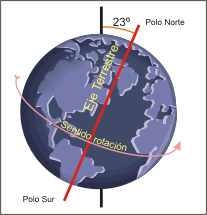
\includegraphics[height=6.5cm]{Imagenes/06.00.navegacion/RotacionTerrestre.png}
 \label{fig:rotacion.tierra}}
  \subfigure[
Precesi\'on
]{
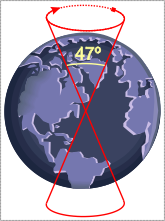
\includegraphics[height=6.5cm]{Imagenes/06.00.navegacion/Precesion.png}
 \label{fig:precesion.tierra}}
  \subfigure[
Nutaci\'on
]{
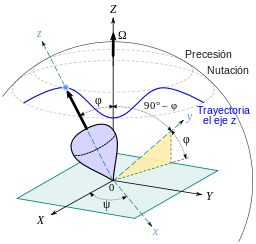
\includegraphics[height=6.5cm]{Imagenes/06.00.navegacion/nutacion.png}
 \label{fig:nutacion.tierra}}
  \subfigure[
Los movimientos \mbox{principales}
]{
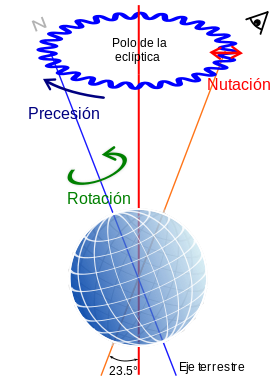
\includegraphics[height=6.5cm]{Imagenes/06.00.navegacion/rotacion-precession-nutation.png}
 \label{fig:los.tres.movimientos.tierra}}

  \caption{La Tierra}
\end{figure}

Dado que el di\'ametro ecuatorial excede al polar en 1 parte sobre 298, se considera que la Tierra es, pr\'acticamente, esf\'erica. 

La Tierra tiene los siguientes movimientos al desplazarse en el espacio:

\begin{itemize}
	\item \textbf{Movimiento de rotaci\'on:} Es un movimiento que efectúa la Tierra girando sobre sí misma a lo largo de un eje ideal denominado Eje terrestre que pasa por sus polos. Una vuelta completa, tomando como referencia a las estrellas, dura 23 horas con 56 minutos y 4 segundos y se denomina día sidéreo. Si tomamos como referencia al Sol, el mismo meridiano pasa frente a nuestra estrella cada 24 horas, llamado día solar. Los 3 minutos y 56 segundos de diferencia se deben a que en ese plazo de tiempo la Tierra ha avanzado en su órbita y debe de girar algo más que un día sideral para completar un día solar, Figura \ref{fig:rotacion.tierra}.

La primera referencia tomada por el hombre fue el Sol, cuyo movimiento aparente, originado en la rotación de la Tierra, determina el día y la noche, dando la impresión que el cielo gira alrededor del planeta. En el uso coloquial del lenguaje se utiliza la palabra día para designar este fenómeno, que en astronomía se refiere como día solar y se corresponde con el tiempo solar.

El eje terrestre forma un ángulo de 23,5º respecto a la normal de la eclíptica, fenómeno denominado oblicuidad de la eclíptica. Esta inclinación produce largos meses de luz y oscuridad en los polos geográficos, además de ser la causa de las estaciones del año, causadas por el cambio del ángulo de incidencia de la radiación solar.

        \item \textbf{Movimiento de traslación:} Es un movimiento por el cual la Tierra se mueve alrededor del Sol. La causa de este movimiento es la acción de la gravedad, originándose cambios que, al igual que el día, permiten la medición del tiempo. Tomando como referencia el Sol, resulta lo que se denomina año tropical, lapso necesario para que se repitan las estaciones del año. Dura 365 días, 5 horas y 47 minutos. El movimiento que describe es una trayectoria elíptica de 930 millones de kilómetros, a una distancia media del Sol de prácticamente 150 millones de kilómetros ó 1 U.A. (Unidad Astronómica). De esto se deduce que la Tierra se desplaza con una rapidez media de 106200 km/h (29,5 km/s).

La trayectoria u órbita terrestre es elíptica. El Sol ocupa uno de los focos de la elipse y, debido a la excentricidad de la órbita, la distancia entre el Sol y la Tierra varía a lo largo del año. A primeros días de enero se alcanza la máxima proximidad al Sol, produciéndose el perihelio, donde la distancia es de 147,5 millones de km,; mientras que en los primeros días de julio se alcanza la máxima lejanía, denominado afelio, donde la distancia es de 152,6 millones de km.

\item \textbf{Movimiento de precesión:} 
también denominado precesión de los equinoccios, es debido a que la Tierra no es esférica, sino un elipsoide achatado por los polos. Si la Tierra fuera totalmente esférica, sólo realizaría los movimientos anteriormente descritos, Figura \ref{fig:precesion.tierra}.

Una vuelta completa de precesión dura 25767 años, ciclo que se denomina año platónico, cuya duración había sido estimada por los antiguos mayas.

\item \textbf{Movimiento de nutación:} debido al achatamiento de los polos y a la atracción de la Luna sobre el eje ecuatorial. También en un movimiento de vaivén y se produce durante el movimiento de precesión, este recorre a su vez una pequeña elipse (como si fuese una pequeña vibración). Una vuelta completa a la elipse suponen 18,6 años, lo que supone que en una vuelta completa de precesión la Tierra habrá realizado 1385 bucles, Figura \ref{fig:nutacion.tierra}.

\item \textbf{Bamboleo de Chandler:} pequeña oscilación del eje de rotación de la tierra que añade 0,7 segundos de arco en un período de 433 días a la precesión de los equinoccios. Fue descubierto por el astrónomo norteamericano Seth Carlo Chandler en 1891, y actualmente no se conocen las causas que lo producen, aunque se han propuesto varias teorías (fluctuaciones climáticas causantes de cambios en la distribución de la masa atmosférica, posibles movimientos geofísicos bajo la corteza terrestre, etc.)


\end{itemize}


\subsection{Coordenadas geogr\'aficas}

El sistema de coordenadas geogr\'aficas determina todas las posiciones de la superficie terrestre utilizando las dos coordenadas angulares de un sistema de coordenadas esf\'ericas que est\'a alineado con el eje de rotaci\'on de la Tierra. Este define dos \'angulos medidos desde el centro de la Tierra:

\begin{itemize}
\item {\bf\Gls{latitud}:} mide el \'angulo entre cualquier punto y el ecuador. Las
  l\'ineas de latitud se llaman paralelos y son c\'irculos paralelos al
  ecuador en la superficie de la Tierra.

  La insolaci\'on terrestre depende de la latitud. Dada la distancia que
  nos separa del Sol, los rayos luminosos que llegan hasta nosotros
  son pr\'acticamente paralelos. la inclinaci\'on con que estos rayos
  inciden sobre la superficie de la Tierra es, pues, variable seg\'un la
  latitud. En la zona intertropical, a mediod\'ia, caen casi verticales,
  mientras que inciden tanto m\'as inclinados cuanto m\'as se asciende en
  latitud, es decir cuanto m\'as nos acercamos a los Polos. As\'i se
  explica el contraste entre las regiones polares, muy fr\'ias y las
  tropicales, muy c\'alidas.


\item {\bf \Gls{longitud}:} mide el \'angulo a lo largo del ecuador desde cualquier   punto de la Tierra. Se acepta que Greenwich en Londres es la
  longitud 0 en la mayor\'ia de las sociedades modernas. Las l\'ineas de
  longitud son c\'irculos m\'aximos que pasan por los polos y se llaman
  meridianos.
\end{itemize}


Combinando estos dos \'angulos, se puede expresar la posici\'on de cualquier punto de la superficie de la Tierra. Por ejemplo, El Cairo, en Egipto, tiene latitud 30 grados norte, y longitud 31 grados este. As\'i un vector dibujado desde el centro de la tierra al punto 30 grados norte del ecuador y 31 grados al este de Greenwich pasar\'a por El Cairo.

El ecuador es un elemento importante de este sistema de coordenadas; representa el cero de los \'angulos de latitud y el punto medio entre los polos. Es el plano fundamental del sistema de coordenadas geogr\'aficas.

\begin{figure}[!h]
  \centering
  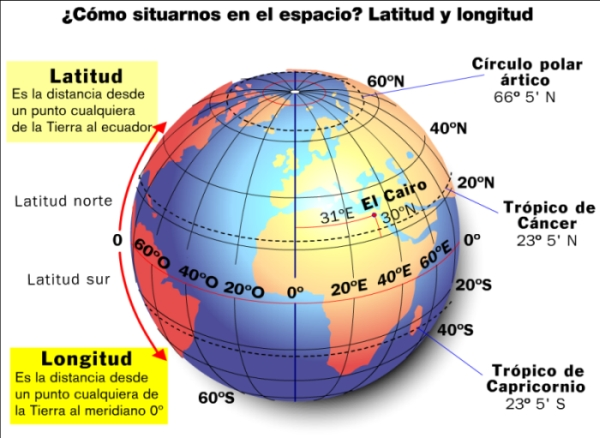
\includegraphics[width=\textwidth]{./Imagenes/06.00.navegacion/latitud_longitud.jpg}
  \caption{Latitud y longitud}
  \label{fig:latitud-longitud}
\end{figure}

El \textbf{Sistema de Coordenadas Universal Transversal de Mercator} (Universal Transverse Mercator, UTM) est\'a basado en un tipo de \gls{proyeccion-cartografica} denominada \emph{proyecci\'on geogr\'afica transversal de Mercator}, tangente a un meridiano. Las magnitudes en el sistema UTM se expresan en metros al nivel del mar, que es la base de la proyecci\'on del elipsoide de referencia.

El sistema de coordenadas UTM fue desarrollado por el Cuerpo de Ingenieros del Ejército de los Estados Unidos en la década de 1940. El sistema se basó en un modelo elipsoidal de la Tierra. Se usó el elipsoide de Clarke de 1866 para el territorio de los 48 estados contiguos. Para el resto del mundo –incluidos Alaska y Hawái– se usó el Elipsoide Internacional. Actualmente se usa el elipsoide WGS84 como modelo de base para el sistema de coordenadas UTM.

Anteriormente al desarrollo del sistema de coordenadas UTM varios países europeos ya habían experimentado la utilidad de mapas cuadriculados, en proyección conforme, al cartografiar sus territorios en el período de entreguerras. El cálculo de distancias entre dos puntos con esos mapas sobre el terreno se hacía más fácil usando el teorema de Pitágoras, al contrario que con las fórmulas trigonométricas que había que emplear con los mapas referenciados en longitud y latitud. En los años de post-guerra estos conceptos se extendieron al sistema de coordenadas basado en las proyecciones Universal Transversa de Mercator y Estereográfica Polar Universal, que es un sistema cartográfico mundial basado en cuadrícula recta.

La proyección transversa de Mercator es una variante de la proyección de Mercator que fue desarrollada por el geógrafo flamenco Gerardus Mercator en 1569. Esta proyección es conforme, es decir, que conserva los ángulos y casi no distorsiona las formas pero inevitablemente sí lo hace con distancias y áreas. El sistema UTM implica el uso de escalas no lineales para las coordenadas X e Y (longitud y latitud cartográficas) para asegurar que el mapa proyectado resulte conforme.

\begin{figure}[!htb]
  \centering
  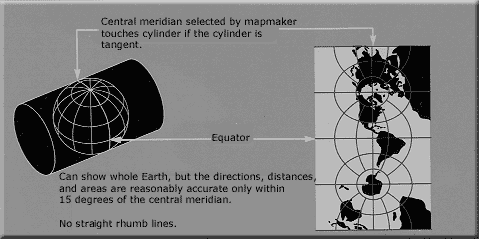
\includegraphics[width=\textwidth]{./Imagenes/06.00.navegacion/Usgs_map_traverse_mercator.png}
  \caption{Sistema de proyecci\'on transversa Mercator}
  \label{fig:sistema.proyeccion.transversa.mercator}
\end{figure}

La UTM es una proyección cilíndrica conforme. El factor de escala en la dirección del paralelo y en la dirección del meridiano son iguales (h = k). Las líneas loxodrómicas se representan como líneas rectas sobre el mapa. Los meridianos se proyectan sobre el plano con una separación proporcional a la del modelo, así hay equidistancia entre ellos. Sin embargo los paralelos se van separando a medida que nos alejamos del Ecuador, por lo que al llegar al polo las deformaciones serán infinitas. Por eso sólo se representa la región entre los paralelos 84ºN y 80ºS. Además es una proyección compuesta; la esfera se representa en trozos, no entera. Para ello se divide la Tierra en husos de 6º de longitud cada uno, mediante el artificio de Tyson .

La proyección UTM tiene la ventaja de que ningún punto está demasiado alejado del meridiano central de su zona, por lo que las distorsiones son pequeñas. Pero esto se consigue al coste de la discontinuidad: un punto en el límite de la zona se proyecta en coordenadas distintas propias de cada Huso.

Para evitar estas discontinuidades, a veces se extienden las zonas, para que el meridiano tangente sea el mismo. Esto permite mapas continuos casi compatibles con los estándar. Sin embargo, en los límites de esas zonas, las distorsiones son mayores que en las zonas estándar.

\begin{itemize}
	\item \textbf{  Husos UTM:}  Se divide la Tierra en 60 husos de 6º de longitud, la zona de
  proyección de la UTM se define entre los paralelos 80º S y 84º
  N. Cada huso se numera con un número entre el 1 y el 60, estando el
  primer huso limitado entre las longitudes 180° y 174° W y centrado
  en el meridiano 177º W. Cada huso tiene asignado un meridiano
  central, que es donde se sitúa el origen de coordenadas, junto con
  el ecuador. Los husos se numeran en orden ascendente hacia el
  este. Por ejemplo, la Península Ibérica está situada en los husos
  29, 30 y 31, y Canarias está situada en el huso 28. En el sistema de
  coordenadas geográfico las longitudes se representan
  tradicionalmente con valores que van desde los -180º hasta casi 180º
  (intervalo -180º → 0º → 180º); el valor de longitud 180º se
  corresponde con el valor -180º, pues ambos son el mismo

\item \textbf{Bandas UTM:}  Se divide la Tierra en 20 bandas de 8º Grados de Latitud, que se
  denominan con letras desde la C hasta la X excluyendo las letras "I"
  y "O", por su parecido con los números uno (1) y cero (0),
  respectivamente. Puesto que es un sistema norteamericano
  (estadounidense), tampoco se utiliza la letra "Ñ". La zona C
  coincide con el intervalo de latitudes que va desde 80º Sur (o -80º
  latitud) hasta 72º S (o -72º latitud). Las bandas polares no están
  consideradas en este sistema de referencia. Para definir un punto en
  cualquiera de los polos, se usa el sistema de coordenadas UPS. Si
  una banda tiene una letra igual o mayor que la N, la banda está en
  el hemisferio norte, mientras que está en el sur si su letra es
  menor que la "N".  

\item \textbf{Notación:} Cada cuadrícula UTM se define mediante el número del huso y la letra
  de la zona; por ejemplo, la Plaza España en la ciudad de C\'ordoba (Argentina) se encuentra en las coordenadas:
  \begin{itemize}
  \item latitud:31º 25' 43.38"  S
  \item longitud:64º 11' 5.84"  W
  \end{itemize}
  las cuales corresponden a las UTM 20J (6523614, 387522), ver Figura \ref{fig:zonas.utm}.  

\item \textbf{Excepciones:}  La rejilla es regular salvo en 2 zonas, ambas en el hemisferio
  norte; la primera es la zona 32V, que contiene el suroeste de
  Noruega; esta zona fue extendida para que abarcase también la costa
  occidental de este país, a costa de la zona 31V, que fue
  acortada. La segunda excepción se encuentra aún más al norte, en la
  zona que se conoce como Svalbard (ver mapa para notar las
  diferencias).
\end{itemize}


\begin{figure}[!htb]
  \centering
  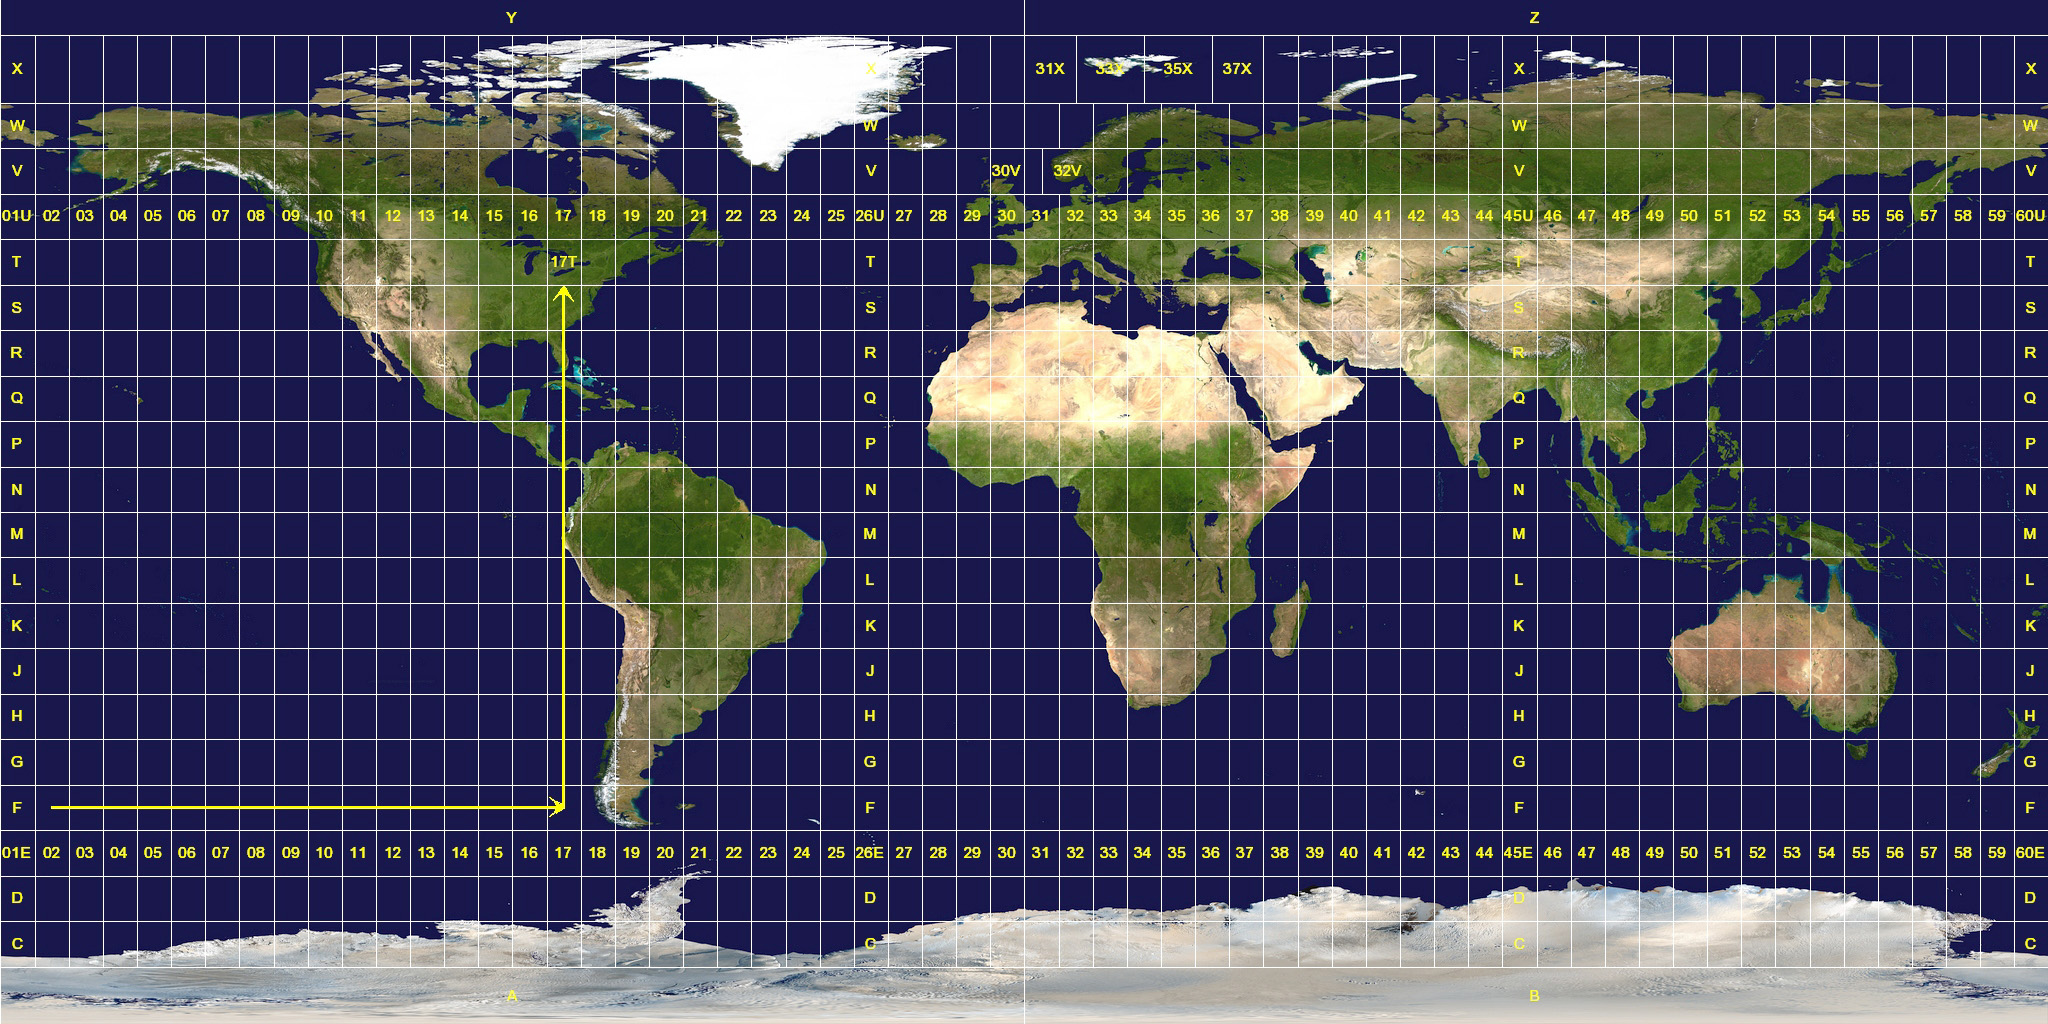
\includegraphics[width=\textwidth]{./Imagenes/06.00.navegacion/Utm-zones.jpg}
  \caption{Zonas UTM}
  \label{fig:zonas.utm}
\end{figure}


\section{Distancia, direcci\'on, tiempo, el Norte}
\label{sec:distancia.direccion.tiempo}

\subsection{Distancia}
\label{sec:distancia}

La distancia se mide como la longitud de la l\'inea que une a dos puntos, su unidad habitual para el uso en navegaci\'on es la \emph{\gls{nauticalmile}} (NM), la cual se define como 1 minuto de latitud o $6076$\,pies ($1852$\,m). A veces es necesario convertir de NM a \gls{statutemile} (SM) y viceversa, lo cual se hace de la siguiente forma:

\[\displaystyle
	\frac{\text{Millas estatutarias}}{\text{Millas n\'auticas}} 
	= \frac{76}{66}
\]

Relacionado con el concepto de distancia se encuentra el de \emph{velocidad}, el cual indica la tasa de cambio de posici\'on. La velocidad se expresa usualmente en millas por hora (mph). Si la medida de la distancia es en NM, entonces la velocidad se expresa en \gls{nudo}. Una velocidad de 200 nudos es igual a una velocidad de 200 NM por hora.

Para calcular la distancia entre puntos sobre la superficie terrestre es necesario tener en cuenta no es plana, lo que implica que existir\'an ligeras (o grandes) distorsiones si se realiza esta operaci\'on sobre un mapa (dependiendo
del tipo de este ultimo).
  
Adem\'as, el hecho de que la Tierra sea un geoide introduce variaciones
adicionales, que deber\'an  (o no) tenerse en cuenta dependiendo de la precisi\'on con que se desee realizar la medici\'on. 

A los fines de una primera aproximaci\'on, puede asumirse que la Tierra es esf\'erica.

Entre dos puntos cualesquiera de la superficie terrestre pueden trazarse líneas curvas diferentes: la ortodrómica, la loxodrómica. %y la isoazimutal.

\begin{description}
\item[Loxodr\'omica \label{loxodromica}]  (del griego   \greektext lox'oc
  % λοξóς
  \latintext ``oblicuo'' y \greektext dr'omoc
  % δρóμος
  \latintext  ``carrera, curso'') a la línea que une dos puntos cualesquiera de la
  superficie terrestre cortando a todos los meridianos con el mismo
  ángulo, ver Figura \ref{fig:loxodromica}. La loxodrómica, por tanto, es fácil de seguir manteniendo el
  mismo rumbo marcado por la brújula. Su representación en el mapa
  dependerá del tipo de proyección del mismo, por ejemplo en la de
  Mercator es una recta.

\item[Ortodrómica \label{ortodromica}] (del griego \greektext enje'ia 
\latintext ``recto'' y
\greektext dr'omoc
 \latintext ''carrera'') es el camino más corto entre dos puntos de la superficie terrestre; es el arco del círculo máximo que los une, menor de 180 grados, Figura \ref{fig:ortodromica}. 

% \item[Isoazimutal] La línea o curva isoazimutal, IsoZ($X,\theta$), es el lugar geométrico de los puntos sobre la superficie terrestre cuyo rumbo inicial ortodrómico respecto a un punto fijo $X$ es constante e igual a $\theta$.

% Es decir, si el rumbo inicial ortodrómico desde S hasta X es de 80 grados, la línea isoazimutal asociada es la formada por todos los puntos cuyo rumbo ortodrómico inicial al punto X es de 80º.
\end{description}

\begin{figure}[!h]
  \subfigure[Loxodr\'omica]{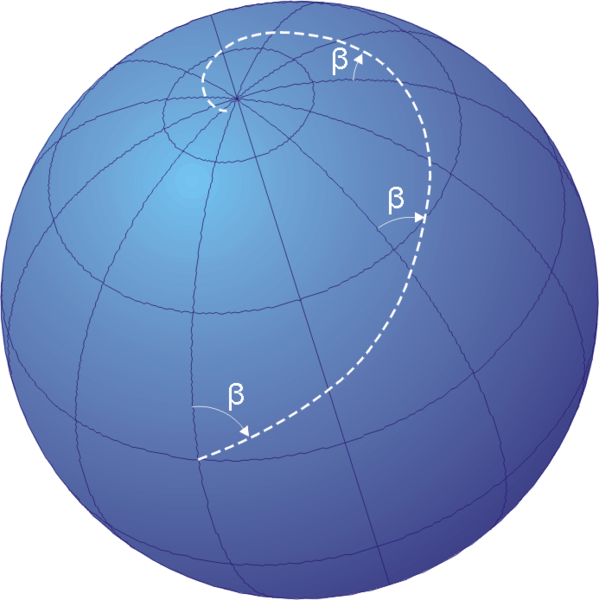
\includegraphics[height=5.8cm]{./Imagenes/06.00.navegacion/loxodromica.png} \label{fig:loxodromica}}
  \subfigure[Ortodr\'omica]{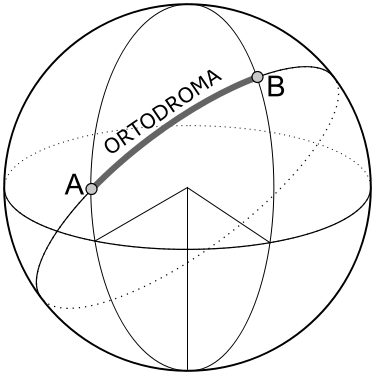
\includegraphics[height=5.8cm]{./Imagenes/06.00.navegacion/ortodroma.png} \label{fig:ortodromica}}
  \subfigure[Comparaci\'on de ambas l\'ineas]{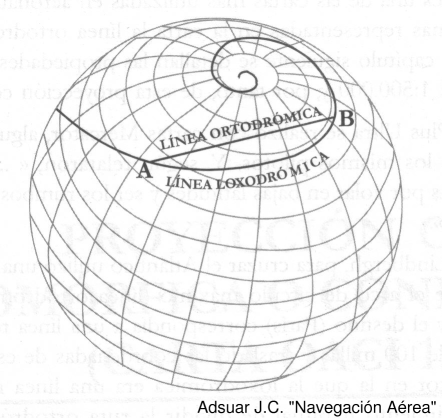
\includegraphics[height=5.8cm]{./Imagenes/06.00.navegacion/comp-loxo-orto.png} \label{fig:ortodromica.loxodromica.comparacion}}
	\caption{Distancia entre dos puntos sobre la Tierra}
\end{figure}

Pedro Nunes, un geógrafo portugués, publicó en Tratado de la navegación (1546) un descubrimiento con grandes implicaciones para la navegación. Antes de él se creía que, marchando sobre la superficie terrestre con un rumbo fijo, es decir, formando un ángulo constante con la meridiana, la línea recorrida era un círculo máximo. Dicho con otras palabras, que un navío que siguiese este derrotero daría la vuelta al mundo y volvería al punto de partida. Nunes señaló la falsedad de este concepto al demostrar que la curva recorrida se va acercando al polo, alrededor del cual da infinitas vueltas, sin llegar nunca a él; o, dicho en lenguaje técnico, que tiene el polo por punto asintótico.

Una característica de la ortodrómica es que presenta un ángulo diferente con cada meridiano, (excepto cuando dicha ortodrómica coincide con un meridiano o con el ecuador). Esta característica representó un grave inconveniente para la navegación, solucionado hacia los últimos años del Siglo XX con el sistema GPS, porque antes del mismo, era difícil trazar una ruta de navegación que siguiera la ortodrómica ya que obligaría a continuos cambios de rumbo. Cuando las distancias eran grandes y seguir el camino más corto suponía un ahorro significativo, se realizaba una aproximación marcando una serie de puntos intermedios, en los cuales se cambiaba de rumbo, y de ésta manera se lograba una aproximación a las correspondientes loxodrómicas.

\subsection{Direcci\'on}
\label{sec:direccion}

La direcci\'on es la posici\'on de un punto en el espacio relativo a otro sin referencia a la distancia entre ellos. En la navegaci\'on se utiliza un sistema n\'umerico para indicar la direcci\'on como el mostrado en la Figura \ref{fig:rosa.de.compas}. En la misma se divide la vista en planta en 360º, comenzando con el norte a 000º y continuando en sentido de las agujas del reloj, pasando por el este a 90º, sur 180º y oeste 270º, volviendo al norte.

Este c\'irculo se denomina rosa de comp\'as, las l\'ineas cuasi-verticales de la Figura \ref{fig:rosa.de.compas} son meridianos. Por el punto A pasa el meridiano a trav\'es de 000º y 180º de la rosa, el punto B se encuentra en una direcci\'on de 60º respecto del A y el punto C en una direcci\'on de 220º del punto A.

\subsubsection{Definiciones}
\label{sec:definiciones.navegacion}

\begin{description}

\item [Trayectoria] (trayectory) se define como el conjunto de puntos del espacio por los cuales pasa la aeronave durante su vuelo (ver Figura \ref{fig:trayectoria}).

\item [Ruta] es la curva resultante de proyectar la trayectoria sobre la superficie de la Tierra (ver Figura \ref{fig:trayectoria}).

\item [Waypoints] son puntos conocidos a lo largo de la ruta, y a menudo resaltan por alguna raz\'on en particular (Lugares de reporte obligatorio, puntos de intersecci\'on de aerov\'ias, etc.) (ver Figura \ref{fig:trayectoria}).

\item [Tramo] (leg) se define como un segmento de ruta comprendido entre dos waypoints (ver Figura \ref{fig:trayectoria}). 

\begin{figure}[!h]
  \centering
  \subfigure[Rosa de comp\'as]{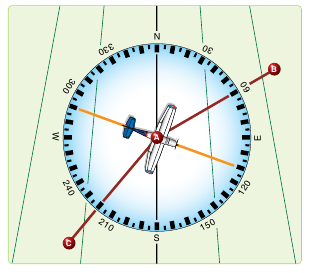
\includegraphics[height=6.7cm]{./Imagenes/06.00.navegacion/rosa.png}  \label{fig:rosa.de.compas}}
  \subfigure[Trayectoria, ruta]{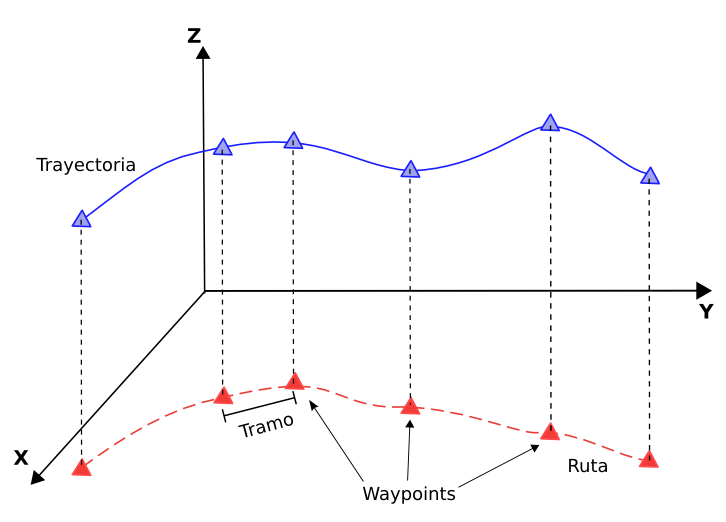
\includegraphics[height=6.7cm]{./Imagenes/06.00.navegacion/trayectoria-ruta.png}  \label{fig:trayectoria}} 

  \caption{Elementos de navegaci\'on}
\end{figure}


  \item[Rumbo] el rumbo o o ``Heading'' (HDG) es el \'angulo entre el norte y el eje   longitudinal de la aeronave (hacia donde apunta su nariz). No
  coincide necesariamente con el vector velocidad (Track) dado que es
  posible, por ejemplo, que el piloto modifique el rumbo para
  contrarestar un viento cruzado (ver Figura \ref{fig:curso}).

\item [Curso deseado] es el \'angulo entre el norte (cualquiera que se est\'e usando: magn\'etico, geogr\'afico, etc) y la l\'inea recta que une dos waypoints sucesivos en la ruta. En ingl\'es se denomina ``\textit{Desired Track}'', y se abrevia DTK (ver Figura \ref{fig:curso}).

\item [Derrota] En n\'autica, la derrota es el trayecto que ha recorrido una embarcaci\'on desde un punto ``\textit{A}'' hasta otro punto ``\textit{B}''. En el derrotero o carta n\'autica se traza la ruta a seguir; contiene informaciones importantes para el navegante, tales como ubicaci\'on de faros, boyas, profundidad del agua, etc. En navegaci\'on a\'erea es el \'angulo entre el norte y la l\'inea tangente a la ruta (dicha tangente corresponde, por cierto, al vector velocidad de la aeronave). En ingl\'es se le llama ``\textit{Track}'' o TK (ver Figura \ref{fig:curso}).

\item [Error transversal] El error transversal o ``\textit{Cross-Track Error}'' (XTE) es la distancia perpendicular entre la posici\'on de la aeronave y la l\'inea que representa al curso deseado. \footnote{Es conveniente tener en cuenta que la diferencia entre el curso deseado (DTK) y la ruta realmente seguida (TK) por lo general es producida por factores externos tales como el viento cruzado (en el caso de las aeronaves) o las corrientes marinas (si se habla de barcos).}

\end{description}

\begin{figure}[!h]
  \centering
  \subfigure[Curso]{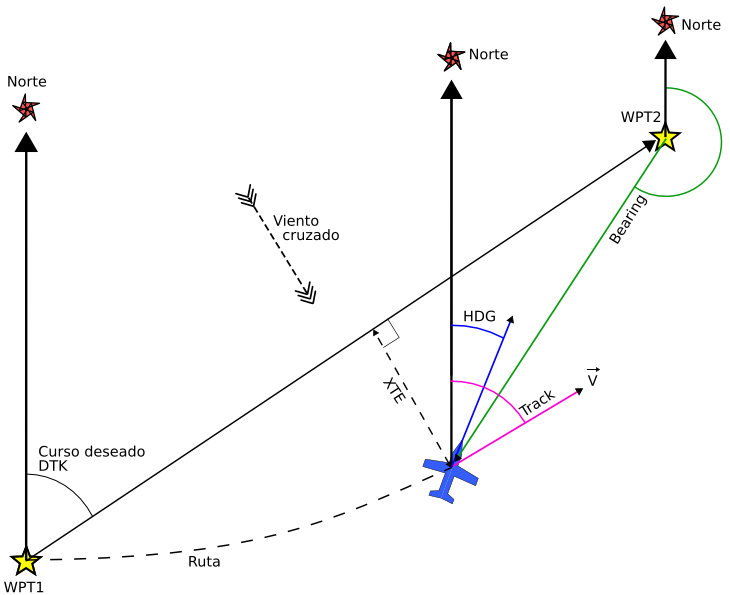
\includegraphics[keepaspectratio,height=10cm]{./Imagenes/06.00.navegacion/curso-derrota-rumbo-marcacion.png}  \label{fig:curso}}
  \caption{Elementos de navegaci\'on (continuaci\'on)}
\end{figure}

\subsection{Tiempo}
\label{sec:tiempo}

La navegaci\'on a\'erea es un problema de cuatro dimensiones: latitud, longitud, altura y es necesario saber \emph{en qu\'e momento} estuvimos (o estaremos) en una posici\'on dada.

Muchos de los sistemas de navegaci\'on modernos est\'an basados en la medici\'on de intervalos de tiempo.

La medici\'on del tiempo se encuentra asociada a la historia del calendario, esto es, un modo sistem\'atico de organizar los d\'ias en semanas, meses, a\~nos y milenios.

Una de las formas m\'as sencillas es con referencia a las fases de la Luna, el calendario de este tipo es denominado \emph{lunar} y el tiempo entre repeticiones de una fase dada de la Luna (p.e., luna nueva) es denominado \emph{mes sin\'odico}. Este dura, en promedio, $29.530589$ d\'ias.

El calendario lunar tiene como ventaja que posee una referencia muy f\'acil de seguir, pero tiene como inconveniente que el mes sin\'odico no tiene un n\'umero entero de d\'ias.

Por otra parte, las estaciones del a\~no son fen\'omenos muy importantes para la vida humana, pero las fases de la Luna son independientes de estas. Por ese motivo algunas culturas prefirieron marcar el paso del tiempo siguiendo el movimiento aparente del Sol por el cielo (ecl\'iptica\footnote{El movimiento que realiza la Tierra en torno al Sol (traslación), genera un plano al que se le ha dado el nombre de Eclíptica. Como el eje de giro de la Tierra tiene una inclinación promedio de 23° 27', entonces el Ecuador terrestre y la eclíptica forma entre si, este mismo ángulo.\\La proyección de la Eclíptica sobre la Esfera Celeste, forma un círculo máximo que se encuentra inclinado con respecto a ella, 23° 27'.
\\ La incidencia perpendicular de los haces de luz solar, barren casi 47º (exactamente 46º 54´) sobre el globo terráqueo. Cuando inciden a 23º 27´ Latitud Norte, alcanzan el denominado Trópico de Cáncer (21 de Junio). Cuando inciden a 23º 27´ Latitud Sur, el Trópico de Capricornio. Estos son los puntos máximos y mínimos que alcanzará el Sol en su desplazamiento imaginario por el cielo. Estos puntos reciben el nombre de Solsticios, del latín Solstitium, que significan “el Sol más lejos”. Los nombres de los Trópicos están determinados por las constelaciones de Cáncer, en el Hemisferio Norte del la Esfera Celeste y de Capricornio, en el Sur.
\\ De manera similar, existen dos puntos en donde se interceptan el Ecuador Celeste y la Eclíptica. Estos son el Punto Vernal  ubicado en la constelación de Los Peces (Piscis) y el Punto Otoñal (d) ubicado en la constelación de La Virgen (Virgo). El Punto Vernal representa en las coordenadas celestes lo que el Meridiano de Greenwich en las coordenadas terrestres, es decir el punto origen de las coordenadas celestes.
\\ En estos dos puntos, los haces de luz solar inciden perpendicularmente sobre el Ecuador de la Tierra, iluminando de manera uniforme a todo el planeta. Estos puntos reciben el nombre de Equinoccios, del latín Aequus Nox, que significa “igual duración de las noches”. En su recorrido anual, la Tierra alcanza estos puntos el 21 de marzo y 21 de Septiembre, respectivamente. }
). Este calendario se denomina \emph{solar}, y el tiempo transcurrido entre dos pasos suscesivos del Sol por el equinoccio de primavera es denominado \emph{a~no vernal equinoxial} y tiene una duraci\'on de $365.2424$ d\'ias.

Se comprob\'o que  19 a\~nos vernales equinoxiales equivalen a $234.997$ meses sin\'odicos ($\approx 235$), lo que implica que cada 19 a\~nos las fases de la Luna y sus fen\'omenos asociados (eclipses) caen casi ex\'actamente en la misma fecha. Este ciclo es denominado \emph{met\'onico} en honor al astr\'onomo Met\'on, siglo V a. C.

Posteriormente los romanos establecieron un calendario que, tras sucesivas adaptaciones, evolucion\'o al calendario actualmente utilizado en el hemisferio occidental, el calendario Gregoriano.

La medici\'on del tiempo tiene, actualmente, dos familias:
\begin{itemize}
\item Las asociadas al movimiento de los cuerpos celestes
\item Las basadas en las oscilaciones de los \'atomos
\end{itemize}

\subsubsection{Tiempo solar}
\label{sec:tiempo.solar}

El tiempo solar es una medida del tiempo fundamentada en el movimiento aparente del Sol sobre el horizonte del lugar. Toma como origen el instante en el cual el Sol pasa por el Meridiano, que es su punto más alto en el cielo, denominado mediodía.1 A partir de este instante se van contando las horas en intervalos de 24 partes hasta que completan el ciclo diurno.

Sin embargo, el Sol no tiene un movimiento regular a lo largo del año, y por esta razón el tiempo solar se divide en dos categorías:

\begin{itemize}
\item {\bf Tiempo solar verdadero} está basado en el día solar verdadero,
  el cual es el intervalo entre dos regresos sucesivos del Sol al
  meridiano. Puede ser medido con un reloj de sol, y se corresponde
  con el amanecer, el mediodía o el anochecer: se basa en lo que es
  posible observar de manera directa. Con un reloj de sol adecuadamente orientado se puede marcar este tiempo, Figura \ref{fig:reloj.de.sol}.

La duración de un día solar verdadero varía a lo largo del año. Esto se debe a que la órbita terrestre es una elipse, con lo cual la Tierra en su movimiento de traslación se mueve más veloz cuando se acerca al Sol y más despacio cuando se aleja de él. Debido a esto, el día solar más corto es el 15 de septiembre, mientras que el día solar más largo es el 22 de diciembre, tanto el Hemisferio Norte como en el Hemisferio Sur.


\item \textbf{ Tiempo solar medio} está basado en un sol ficticio que viaja a una   velocidad constante a lo largo del año, y es la base para definir el
  día solar medio (24 horas u $86400$ segundos). Se corresponde con el
  tiempo civil y se coordina mediante el Tiempo Medio de Greenwich.
\end{itemize}


La diferencia entre el tiempo solar verdadero y el tiempo solar medio, que en ocasiones llega a ser de 15 minutos, es llamada \emph{Ecuación de tiempo}, Figura \ref{fig:2012.ecuacion.del.tiempo}.


\begin{figure}[!h]
  \centering
  \subfigure[Reloj de sol]{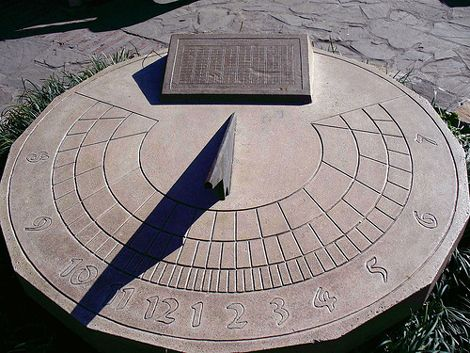
\includegraphics[height=6.5cm]{./Imagenes/06.00.navegacion/reloj-de-sol.jpg} \label{fig:reloj.de.sol}}
  \subfigure[Ecuaci\'on del tiempo, a\~no 2012]{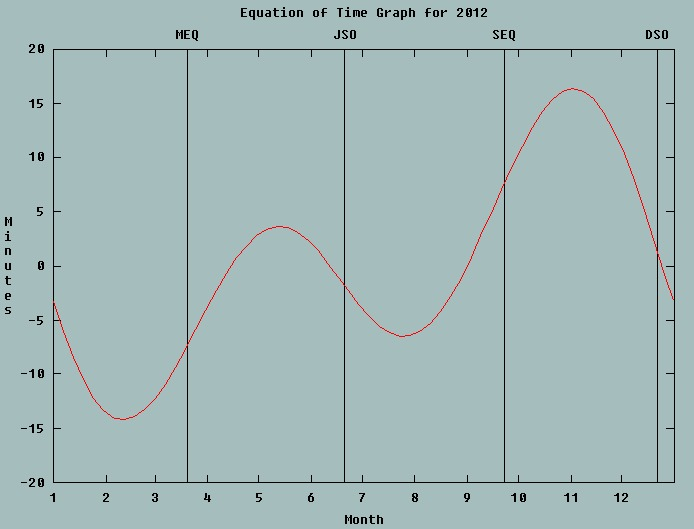
\includegraphics[height=6.5cm]{./Imagenes/06.00.navegacion/2012-ecuacion-tiempo.jpg} \label{fig:2012.ecuacion.del.tiempo}}

  \subfigure[Meridiano de Greenwich]{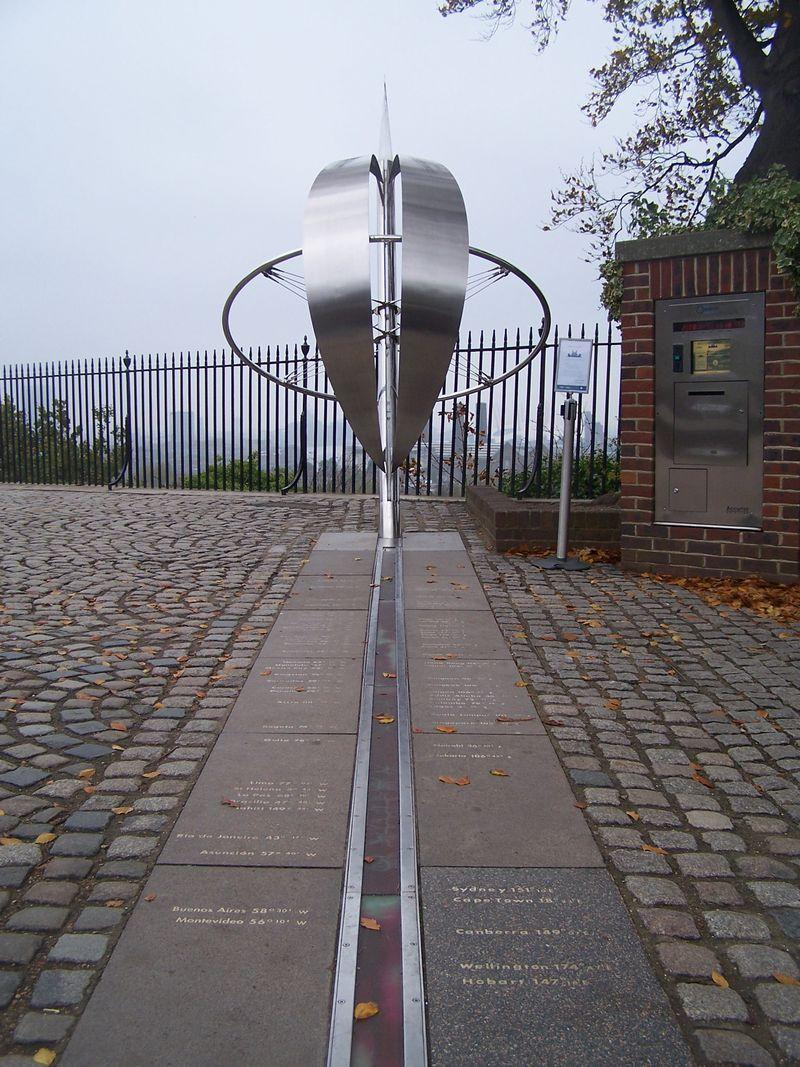
\includegraphics[height=6.5cm]{./Imagenes/06.00.navegacion/Greenwich-Meridian-Line.jpg} \label{fig:meridiano.greenwich}}
  \subfigure[Primer reloj at\'omico (1948)]{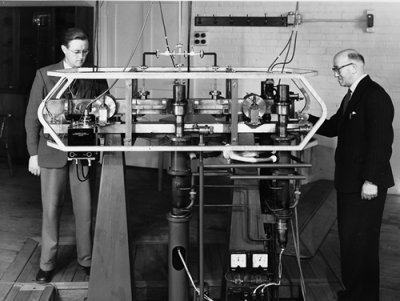
\includegraphics[height=6.5cm]{./Imagenes/06.00.navegacion/TAI.jpg} \label{fig:primer.reloj.atomico}}

  \caption{Medici\'on del tiempo}
\end{figure}

\subsubsection{ Greenwich Mean Time}
\label{sec:greenwich.mean.time}

El  Greenwich Mean Time (GMT)  es una escala de tiempo basada en el paso
del Sol Medio por el meridiano de Greenwich (espec\'ificamente por el viejo
Observatorio Real de Greenwich, que es el punto de referencia).
Este tiempo est\'a  obsoleto pues en 1928 la Uni\'on Astron\'omica 
 Internacional introdujo el  Universal Time (UT) para reemplazarlo.

\subsubsection{Tiempo Universal (UT)}
\label{sec:tiempo.universal}

El UT reemplaz\'o al GMT puesto que este \'ultimo se basaba en la medici\'on de la posici\'on del Sol, y existen problemas asociados a la medici\'on precisa de la misma.

El UT se basa en la medici\'on de la posici\'on de referencias astron\'omicas, como los cu\'asares, consigui\'endose mayor precisi\'on.

 A pesar de su mayor precisión el UT sigue siendo una escala de tiempo no uniforme, pues en el fondo se basa en la medición del período de rotación del planeta y éste presenta anomalías. De hecho, en 1956 el Comité Internacional de Pesos y Medidas decidió que la definición del segundo se haría en función del período de revolución de la Tierra para una época dada, y así el segundo de efemérides fue definido como:

La fracción 1/31556925,9747 del año tropical medio para el 1ro. de Enero de 1900 a las 12 horas.

Debido a la existencia de las mencionadas anomalías, existen varios tipos de UT:
\begin{description}

\item [UT0:] Es el Tiempo Universal definido mediante observaciones de
  puntos de referencia astronómicos. Inicialmente era medido mediante
  relojes de péndulo, pero conforme la tecnología de los relojes fue
  avanzando, se notó la existencia de errores.


\item [UT1:] Cuando a UT0 se le aplican las correcciones debidas al
  movimiento de los polos (efecto Chandler y otros) obtenemos
  UT1. Esta escala es la más ampliamente utilizada por los astrónomos
  y a menudo el término UT se refiere a ella.


\item [UT2:] Debido a que la velocidad de rotación de la Tierra no es
  constante, UT1 presenta variaciones estacionales relacionadas, entre
  otras cosas, a las mareas y el intercambio de energía entre la
  Tierra y la atmósfera. Al aplicar las correcciones debidas a las
  variaciones más fuertes y regulares (del orden de 3 milisegundos por
  día), obtenemos UT2. Esta escala, la más precisa para el Tiempo
  Universal, sigue siendo irregular y por ello ha caído en desuso
  después de la aparición de nuevos métodos no astronómicos para la
  medición del tiempo.
\end{description}


\subsubsection{ Temps Atomique International (TAI)}
\label{sec:temps.atomique.international}

 Dado que las escalas de tiempo anteriores no eran suficientemente regulares, se desarrollaron relojes cada vez más precisos que permitieron desligarse de la rotación de la Tierra como patrón que definía el tiempo. Estas investigaciones desembocaron en el reloj atómico, que marca el tiempo examinando el comportamiento de los átomos de un material dado, y por tanto la escala de tiempo así construida no depende (o depende muy poco) de factores externos.

Desde mediados de 1950 se empezaron a desarrollar relojes atómicos suficientemente precisos y por ello la 13ra. Conferencia General de Pesos y Medidas celebrada en el año 1967 pudo definir el segundo del Sistema Internacional como:

\vspace{3mm}

\fbox{\parbox{\textwidth}{La duración de 9192631770 períodos de la onda de la radiación emitida por el átomo de Cesio 133 cuando se realiza la transición entre los dos niveles hiperfinos del estado fundamental del átomo.}}

\vspace{3mm}

En función de esta definición, la BIPM (Oficina Internacional de Pesos y Medidas), localizada en París, Francia, coordina y promedia los datos provenientes de un gran número de relojes atómicos alrededor del globo para generar una escala de tiempo uniforme llamada TAI (Tiempo Atómico Internacional). 



\subsubsection{Tiempo Universal Coordinado (UTC)}
\label{sec:tiempo.universal.coordinado}
 El UTC es una escala de tiempo atómica internacional ampliamente utilizada en el ámbito civil. De hecho, hoy en día prácticamente todos los países del mundo definen sus horas locales en función de UTC6.9, añadiendo o restando un número entero de horas según convenga a su localización geográfica.

En cierta forma, UTC puede verse como la manera de reconciliar el tiempo atómico (TAI) con el tiempo dado por la rotación de la Tierra (Tiempo Universal \#1 - UT1).

UTC tiene la misma frecuencia del TAI pero cada cierto tiempo se le añaden (o sustraen) segundos extras (llamados ``leap seconds'') para mantenerlo sincronizado dentro de +/- 0,9 s de UT1. De esta manera, se obtiene la exactitud del tiempo atómico sin divorciarse completamente del fenómeno de la rotación terrestre.

Los ``leap seconds'' empezaron a usarse el 30 de Junio de 19726.10, y habitualmente se introducen al final del último minuto del último día de diciembre o del último día de junio, si hace falta. Hasta el momento6.11 se han introducido 33 s (todos ellos de retraso).

\subsubsection{Tiempo GPS (GPST)}
\label{sec:tiempo.gps}


También llamado GPST, el tiempo GPS es el utilizado como referencia para las aplicaciones relacionadas con el sistema de posicionamiento global por satélite del Departamento de Defensa de los EE.UU.

El GPST es un tiempo de naturaleza atómica que no es alterado por ``leap seconds''. Toma como época de origen las 00:00 UTC de la noche del 5 al 6 de enero de 1980. Dado que para esa fecha se habían introducido 19 ``leap seconds'', la siguiente expresión es válida:

TAI - GPST = 19 s

Un concepto adicional importante es la llamada semana GPS. Ésta empieza la noche del sábado al domingo, de modo tal que el 17 de marzo del 2004 correspondió a la semana GPS 1262. Las semanas GPS tienen un ciclo de 1024, y el primer ciclo se alcanzó en la noche del 21 al 22 de Agosto de 1999, llamado ``GPS Week Rollover''. 

\subsubsection{Tiempo Loran-C}
\label{sec:tiempo.loran.c}

%El término LORAN, que significa ``Long Range Navigation'' (Navegación de Largo Alcance), co\-rres\-pon\-de a una cadena de transmisores de radiofrecuencia de amplio alcance que permiten conocer con cierta precisión (aproximadamente 0,25 NM) la posición de un receptor sobre la superficie terrestre.

Los transmisores pertenecientes a la cadena (o ``chain'', en inglés) Loran poseen relojes atómicos que están sincronizados entre sí. Estos relojes no son alterados por ``leap seconds'', lo que hace que se separe progresivamente de UTC.

La época de inicio de los relojes atómicos del sistema Loran-C fue las 0h del 01/Ene/1958.

\subsection{El Norte}
\label{sec:el.norte}
El concepto de ``\emph{Norte}'' engloba una serie de definiciones que es necesario conocer y diferenciar adecuadamente:

\begin{itemize}
\item\textbf{ Norte geográfico: }Es el que viene dado por la intersección del eje de rotación de la Tierra con la superficie de la misma [1]. Es llamado también "Norte verdadero", y en él confluyen todos los meridianos.

\item \textbf{Norte magnético:} Es el punto donde la mayor parte de las líneas de fuerza del campo magnético terrestre entran en la superficie. Se puede detectar utilizando instrumentos tales como la brújula y la "flux valve" (equivalente a la brújula en las aeronaves modernas).

Es importante hacer notar que el norte geográfico y el magnético \textbf{NO} coinciden, y que además el norte magnético cambia su posición con el tiempo.

\item \textbf{Declinación magnética:} Es el ángulo de desviación entre las posiciones del norte magnético y geográfico, vistas desde un punto en particular. Se denota como D y se considera positiva cuando el ángulo medido está hacia el Este del norte verdadero, y negativo en caso contrario. 

Lo anterior significa que si sobre un punto de la superficie terrestre la brújula marca un rumbo de 115º, y sabemos que la declinación magnética en ese punto es 4º E, el rumbo verdadero serán 119º. 

En la Figura \ref{fig:declinacion-magnetica} se representa la declinación magnética para dos puntos diferentes de la superficie terrestre. Note que en uno de ellos la geometría es tal que la declinación es cero. 

\begin{figure}[!h]
    \centering
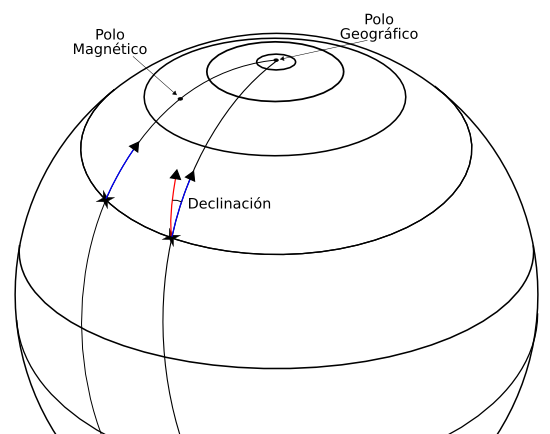
\includegraphics[keepaspectratio,width=0.6\textwidth]{./Imagenes/06.00.navegacion/declinacion-magnetica.png}
\caption{Declinaci\'on magn\'etica en dos puntos diferentes de la Tierra \cite{Salazar_nav_aerea}}
\label{fig:declinacion-magnetica}
\end{figure}

\item \textbf{Líneas isógonas:} Se llaman así a las líneas que, sobre las cartas de navegación o los mapas, unen puntos que tienen la misma declinación magnética. Son también denominadas Líneas Isogónicas. Adicionalmente, si una línea corresponde a puntos con declinación 0º, se habla de Línea Agónica. 

\item \textbf{Norte de la Brújula:} Es el norte magnético tal y como lo indica a bordo el instrumento adecuado (brújula o flux valve). No indica realmente el norte magnético pues el instrumento comete errores por diversas razones (presencia de masas metálicas cercanas, líneas de campo magnético que no son horizontales, etc).

\item \textbf{Desviación magnética:} Es el error angular cometido por la brújula o flux valve. El fabricante de la aeronave puede corregirla hasta cierto punto.

La Figura \ref{fig:declinacion-desviacion} presenta la relación entre los nortes geográfico, magnético y de la brújula con sus correspondientes diferencias angulares.

\begin{figure}[!htb]
    \centering
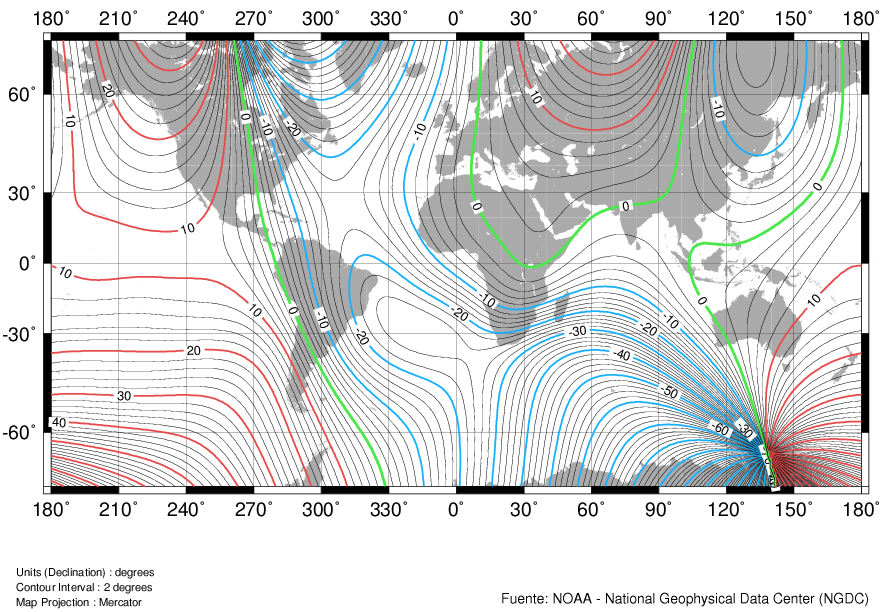
\includegraphics[keepaspectratio,width=\textwidth]{./Imagenes/06.00.navegacion/declinacion-magnetica-anio-2000.png}
\caption{Declinaci\'on magn\'etica - A\~no 2000 \cite{Salazar_nav_aerea}}
\label{fig:declinacion-magnetica-anio-2000}
\end{figure}

\begin{figure}[!htb]
    \centering
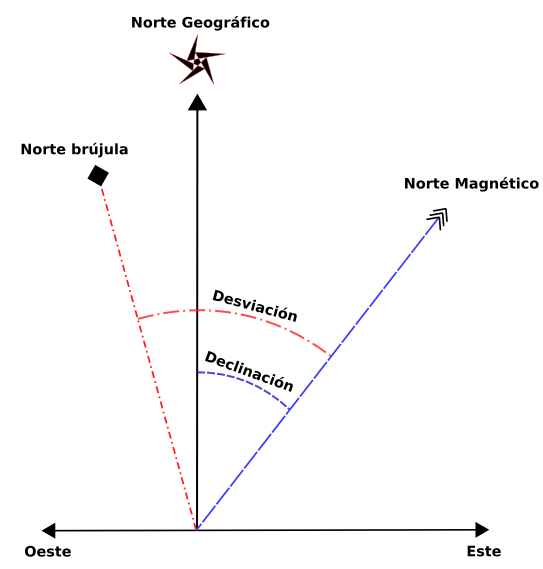
\includegraphics[keepaspectratio,width=0.6\textwidth]{./Imagenes/06.00.navegacion/declinacion-desviacion.png}
\caption{Los diferentes nortes y sus diferencias angulares \cite{Salazar_nav_aerea}}
\label{fig:declinacion-desviacion}
\end{figure}


\item \textbf{Norte de la Cuadrícula:} Cuando se navega a grandes latitudes (muy al norte o muy al sur del planeta), no tiene sentido guiarse por el norte magnético debido, entre otras cosas, a las grandes declinaciones implicadas.

Es por ello que se define arbitrariamente el Norte de la Cuadrícula como el norte indicado por los meridianos de la carta de navegación que se está usando para navegar. 
\end{itemize}





\section{Cartas de navegaci\'on aeron\'autica}
\label{sec:cartas.navegacion.aeronautica}

La carta aeron\'autica se define como la representaci\'on de una porci\'on de la tierra, su relieve y construcciones, dise\~nada especialmente para satisfacer los requisitos de la navegaci\'on a\'erea. Se trata de un mapa en el que se reflejan las rutas que deben seguir las aeronaves, y se facilitan las ayudas, los procedimientos y otros datos imprescindibles para el piloto.

El gran problema asociado a la construcción y utilización de cartas es que la superficie de la Tierra \textbf{no se puede representarse con fidelidad en ninguna carta}. Esto se debe a que una esfera \emph{no es una superficie desarrollable}, es decir, no es posible convertirla a un plano sin generar distorsiones. Es el mismo problema que enfrentaríamos si intentáramos convertir la cáscara de una naranja en un plano sin alterarla, Figura \ref{fig:comparacion.proyecciones.cartograficas}. 

Superficies que sí son desarrollables son los cilindros y los conos. En ambos casos, basta con cortar dichas superficies por un lugar conveniente y seguidamente las podemos estirar sin deformarlas y convertirlas en planos.

Por esta razón, la práctica común al construir una carta consiste en proyectar la superficie de la Tierra sobre una de estas tres superficies (plano, cono o cilindro). Dicha proyección consiste en escoger un conjunto de reglas geométricas y aplicarlas sistemáticamente a toda la superficie que se interesa proyectar, Figura \ref{fig:proyecciones.cartograficas}.

\subsection{Proyecciones cartogr\'aficas}
\label{sec:proyecciones.cartograficas}

Como las cartas de navegación en realidad son proyecciones de la superficie terrestre, es conveniente estudiar primero las características de las proyecciones para entender luego las de las cartas. 

 Existe un gran número de tipos diferentes de proyecciones según el conjunto de reglas que se escojan para hacerla (por ejemplo: punto de origen, tipo de superficie de proyección, posición de la superficie, etc.). Cada uno de estos conjuntos de reglas introduce diferentes tipos de distorsiones, que son inevitables, y en base a éstas se puede a su vez definir diferentes propiedades de la proyección.

\begin{figure}[!h]
  \centering
  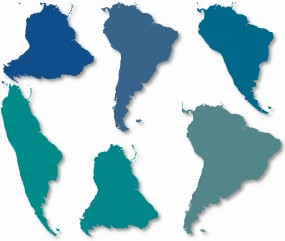
\includegraphics[width=0.8\textwidth]{./Imagenes/06.00.navegacion/comparacion-proyecciones.jpg}
  \caption{Am\'erica del Sur en diferentes proyecciones. ¿Cu\'al es la correcta? \\{\footnotesize Fuente: \url{http://www.progonos.com/furuti/MapProj/Normal/TOC/cartTOC.html}}}
  \label{fig:comparacion.proyecciones.cartograficas}
\end{figure}


La razón de que existan tantos tipos de proyecciones diferentes es que estas propiedades las hacen adecuadas para un uso u otro, según lo que se desee. En las siguientes secciones estudiaremos las propiedades más importantes que pueden tener las proyecciones, y por ende, las cartas hechas con ellas. 

\begin{figure}[!h]
  \centering
  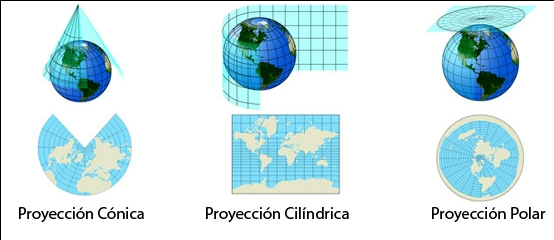
\includegraphics[width=\textwidth]{./Imagenes/06.00.navegacion/proyecciones.jpg}
  \caption{Proyecciones cartogr\'aficas}
  \label{fig:proyecciones.cartograficas}
\end{figure}

Entre las propiedades de las proyecciones se tiene:

\begin{description}
\item[Conformidad] Un mapa conforme es aquél que preserva los ángulos (y por tanto, las formas) a nivel local. Esto significa que las formas de características tales como deltas, ríos, etc. son reconocibles, pues la distorsión que sufren no es grande.
\item[Equivalencia] Una proyección es equivalente o autálica si mantiene las proporciones entre las áreas representadas. Esto quiere decir que si un país dado A tiene el doble del área que un país B, en una proyección equivalente dicha proporción se mantiene, Figura \ref{fig:groenlandia.africa.comparacion.superficies.segun.tipo.proyeccion}. 

Las proyecciones equivalentes o autálicas son de escasa utilidad para la navegación, pero por otra parte son muy útiles cuando se quiere presentar información que ha de compararse a simple vista, como población, producción industrial, etc., o para elaborar atlas escolares.


\begin{figure}[!h]
  \centering
  \subfigure[Proyeccion Mercator]{
  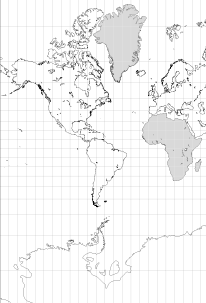
\includegraphics[height=7cm]{./Imagenes/06.00.navegacion/merEqTh.png}
  \label{fig:proyeccion.mercator.groenlandia.africa}
  }
  \subfigure[Proyeccion Mollweide]{
  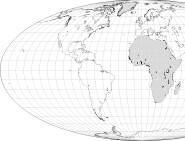
\includegraphics[height=7cm]{./Imagenes/06.00.navegacion/mollEqTh.png}
  \label{fig:proyeccion.mollweide.groenlandia.africa}
  }
  \caption{Comparaci\'on de las superficies de Groenlandia y \'Africa seg\'un el tipo de proyecci\'on utilizada, superficie \'Africa = 29800000\,km$^2$, superficie Groenlandia = 2175600\,km$^2$\\{\footnotesize Fuente: \url{http://www.progonos.com/furuti/MapProj/Normal/CartProp/AreaPres/areaPres.html}}
}
  \label{fig:groenlandia.africa.comparacion.superficies.segun.tipo.proyeccion}
\end{figure}


\item[Equidistancia] Una proyección es equidistante cuando posee un conjunto bien definido y completo de líneas a lo largo de las cuales la escala se mantiene constante, Figura \ref{fig:proyeccion.equidistante}.

Al indicar que posee un conjunto bien definido y completo de líneas, nos referimos al hecho de que muchas proyecciones tienen unas pocas líneas a lo largo de las cuales la escala se mantiene constante (a menudo llamadas líneas automecoicas. No obstante, en las cartas equidistantes el número de líneas que tienen esta propiedad es mucho más grande.

Por ejemplo, es posible crear una carta con una proyección equidistante que esté centrada en una ciudad dada A, y entonces se podría calcular con exactitud la distancia entre tal ciudad A y cualquier otra ciudad que se represente en la carta.

Las cartas equidistantes a menudo distorsionan mucho los ángulos y áreas, y por ello tienen una utilidad limitada. Sin embargo es posible obtener pocas distorsiones si el área representada es pequeña. 

    \begin{figure}[!h]
      \centering
  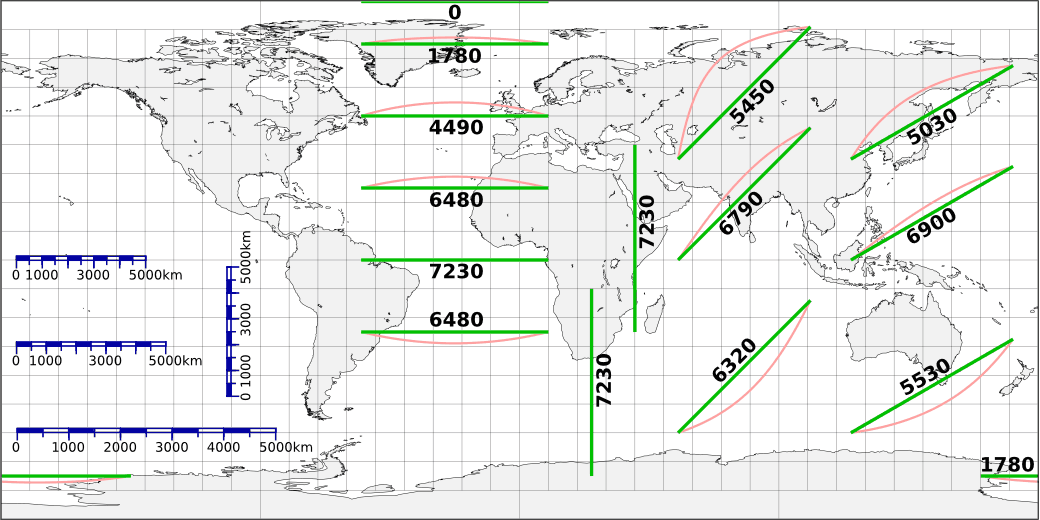
\includegraphics[height=9cm]{./Imagenes/06.00.navegacion/proyeccion-equidistante.png}
      \caption{Proyecci\'on equidistante cil\'indrica, distancias en km. Cada escala gr\'afica es v\'alida a lo largo de su propio paralelo. Solo la escala vertical es v\'alida en cualquier lugar.\\{\footnotesize Fuente: \url{http://www.progonos.com/furuti/MapProj/Normal/CartProp/AreaPres/areaPres.html}}}
      \label{fig:proyeccion.equidistante}
    \end{figure}


\item[Dirección]  Otra propiedad importante de las proyecciones es la referida a si distorsionan, y de qué manera, las direcciones. Por ejemplo, una proyección que muestra de forma correcta todas las direcciones desde su centro a cualquier otro punto de la carta se llama azimutal.

Hay al menos dos maneras diferentes de entender la dirección: En función del círculo máximo y en función del rumbo, y ambas maneras definen líneas muy importantes: 

\begin{description}
	\item[Líneas Loxodrómicas] ver  \fullref{loxodromica}
	\item[Líneas Ortodrómicas] ver \fullref{ortodromica}
\end{description}

En la Figura \ref{fig:comparacion.entre.loxodromas.y.ortodromas} puede observarse una comparaci\'on entre este tipo de l\'ineas al conectar dos puntos.

\begin{figure}[!h]
  \centering
  \subfigure[Proyecci\'on Mercator]{
	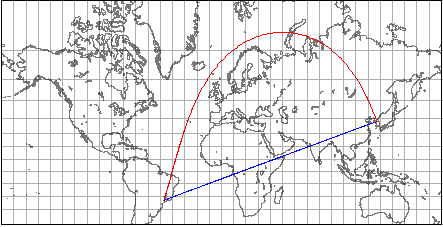
\includegraphics[height=6cm]{./Imagenes/06.00.navegacion/gr-mr-s70-n80-s-40.png}
	}
  \subfigure[Proyecci\'on polar azimutal equidistante]{
	\includegraphics[height=6cm]{./Imagenes/06.00.navegacion/gr-aze-s70.png}
	}
  \subfigure[Proyecci\'on Lagrange]{
	\includegraphics[height=6cm]{./Imagenes/06.00.navegacion/lg-s70h.png}
	}
  \caption{Comparaci\'on entre loxodromas y ortodromas, azul loxodromica, rojo ortodromica \\{\footnotesize Fuente: \url{http://www.progonos.com/furuti/MapProj/Normal/ShapePres/shapePres.html}}}
  \label{fig:comparacion.entre.loxodromas.y.ortodromas}
\end{figure}

\end{description}

\subsection{Las cartas OACI \cite{Salazar_nav_aerea}}

La seguridad de la navegaci\'on a\'erea exige la elaboraci\'on y publicaci\'on de cartas aeron\'auticas actualizadas y precisas, que respondan a las necesidades actuales de la aviaci\'on. En consecuencia, corresponde a cada Estado miembro de la Organizaci\'on de Aviaci\'on Civil Internacional (OACI) adoptar las disposiciones necesarias para facilitar el esfuerzo de cooperaci\'on que supone la producci\'on y difusi\'on de cartas aeron\'auticas. Adem\'as, cada Estado tiene la obligaci\'on de proporcionar informaci\'on del propio territorio a trav\'es de las cartas aeron\'auticas.

La Organizaci\'on de Aviaci\'on Civil Internacional (OACI), en su Anexo 4 - Cartas Aeron\'auticas, ha publicado una serie de normas y m\'etodos recomendados para la elaboraci\'on de las mismas. Adicionalmente, y como complemento y ayuda para la puesta en pr\'actica de estas normas, tambi\'en proporciona el Manual de Cartas Aer\'onauticas.

Seg\'un la OACI, el dise\~no de las cartas aeron\'auticas debe tomar en cuenta una serie de factores, entre los cuales se pueden mencionar:

\begin{itemize}

\item  Debe utilizarse una proyecci\'on com\'un.

  \item Las escalas utilizadas deben tener valores f\'acilmente
  comprensibles.

  \item Debe facilitarse la transici\'on de una carta a otra durante el
  vuelo mediante una adecuada selecci\'on de alturas, construcciones u
  otra informaci\'on relativa al terreno.

  \item Deber\'ian publicarse simult\'aneamente las cartas que tienen conexi\'on
  entre s\'i, ya sean cartas nuevas o sus revisiones.

\end{itemize}

\begin{landscape}
  \newcommand{\minitab}[2][1]{\begin{tabular}{#1}#2\end{tabular}}
Cartas opcionales. Las seis cartas opcionales se producir\'an si, en opinión de las Autoridades aeron\'auticas de los Estados, contribuyen a la seguridad, regularidad y eficacia de las operaciones de las aeronaves.

Cartas condicionales. Las cinco cartas condicionales se producir\'an solamente si se cumplen determinadas condiciones o circunstancias.

\begin{table}%[!h]
  \centering
  \caption{Cartas aeron\'auticas OACI}
  \label{tab:cartas.aeronauticas.OACI}
  \begin{small}
    \begin{tabular}{|m{0.12\textheight}|m{0.4\textheight}|c|c|c|m{0.35\textheight}|}
      \cline{3-5} 
	\multicolumn{2}{c|}{} & %\multirow{2}*[1.5cm]{
      \begin{turn}{90}
        \textbf{Obligatoria}
      \end{turn}
      % }
      &%\multirow{2}*[1.5cm]{
      \begin{turn}{90}
        \textbf{Opcional}
      \end{turn}
      % }
      &%\multirow{2}*[1.5cm]{
      \begin{turn}{90}
        \textbf{Condicional \,}
      \end{turn}
      % } 
      & \multicolumn{1}{c}{}
      \\ \cline{1-2}\cline{6-6}
      \centering \textbf{Grupo} & \centering \textbf{Carta} & 
      & & &\multicolumn{1}{c|}{\textbf{Requerimientos}}\\ \hline

      \multirow{4}{0.12\textheight}{ Planificaci\'on previa al vuelo} &
      \parbox{\linewidth}{1. Plano de obst\'aculos de aeródromo – Tipo A \\
      (limitadores de utilización).} 
	&\cellcolor{red} & & &
       Aeródromos con obst\'aculos destacados en las \'areas de despegue y aterrizaje.
	\\
&&&&& \\
&&&&& \\
&&&&& \\

%       \multirow{4}{0.12\textwidth}{ Planificaci\'on previa al vuelo} &
%       \minitab[l]{1. Plano de obst\'aculos de aeródromo – Tipo A \\
%       \quad (limitadores de utilización).} &\cellcolor{red} & & &
%        Aeródromos con obst\'aculos destacados en las \'areas de despegue y aterrizaje.
% 	\\
%       &
%       2. Plano de obst\'aculos de aeródromo – Tipo B. & &\cellcolor{blue} & & \\
%       &
%       3. Plano de obst\'aculos de aeródromo – Tipo C.& & &\cellcolor{green} & \\
%       &
%       4. Carta topogr\'afica para aproximaciones de precisión. &\cellcolor{red} & & & Obligatoria en pistas con aproximaciones de precisión categorías II y III\\ \hline
%       \multirow{4}{0.12\textwidth}{ En vuelo} &
%       5. Carta de navegación en ruta. &\cellcolor{red} & & & 
% 	Zonas en las que se hayan establecido Regiones de Información de Vuelo (FIR)	\\
%       &
%       6. Carta de \'area. & & &\cellcolor{green} & \\
%       &
%       7. Carta de salida normalizada – Vuelo por instrumentos (SID). & & &\cellcolor{green} & \\
%       &
%       8. Carta de llegada normalizada – Vuelo por instrumentos (STAR). & & &\cellcolor{green} & \\
%       &
%       9. Carta de aproximación por instrumentos. &\cellcolor{red} & & &
% Aeródromos en los que se haya establecido tal tipo de aproximación \\
%       &
%       10. Carta de aproximación visual.  & & &\cellcolor{green} & \\ \hline
%       \multirow{4}{0.12\textwidth}{Movimientos en tierra %de 
%         %	las aeronaves en el aeródromo
%       } &
%       11. Plano de aeródromo/helipuerto &\cellcolor{red} & & & 
% En todos los que se utiliza regularmente la aviación civil internacional\\
%       &
%       12. Plano de aeródromo para movimientos en tierra.  & &\cellcolor{blue} & & \\
%       &
%       13. Plano de estacionamiento y atraque de aeronaves.  & &\cellcolor{blue} & & \\ \hline
%       \multirow{4}{0.12\textwidth}{Navegación a\'erea visual, trazado de posiciones, planificación} &
%       14. Carta aeron\'autica mundial (escala 1:1.000.000). & \cellcolor{red}& & & En todas las zonas especificadas por la OACI\\
%       &
%       15. Carta aeron\'autica (escala 1:500.000).  & &\cellcolor{blue} & & \\
%       &
%       16. Carta de navegación aeron\'autica (escala peque\~na). & &\cellcolor{blue} & & \\
%       &
%       17. Carta de posición.  & &\cellcolor{blue} & & \\ \hline

    \end{tabular}
  \end{small}
\end{table}
\end{landscape}

\subsubsection{Cartas OACI obligatorias}

El Anexo 4 exige que cada pa\'is garantice la disponibilidad de seis (6) 
tipos diferentes de cartas aeron\'auticas que se consideran obligatorias:

\begin{enumerate}

\item   Plano de obst\'aculos de aer\'odromo - OACI, Tipo A: Para aquellos
  aer\'odromos donde hay obst\'aculos destacados en el \'area de la
  \gls{trayectoria} de despegue.

  \item. Carta topogr\'afica para aproximaciones de precisi\'on - OACI: Para
  todos los aer\'odromos con pistas de aproximaci\'on de precisi\'on de
  Categor\'ias II y III.

  \item Carta de navegaci\'on en ruta - OACI: Para todas las zonas donde se
  hayan establecido regiones de informaci\'on de vuelo (FIR).

  \item Carta de aproximaci\'on por instrumentos - OACI: Para aquellos
  aer\'odromos donde se hayan establecido procedimientos de aproximaci\'on
  instrumentales.

  \item Plano de Aer\'odromo/Helipuerto - OACI: Necesario para todos
  aquellos aer\'odromos/helipuertos regularmente utilizados por la
  aviaci\'on civil internacional.

  \item Carta aeron\'autica mundial - OACI, 1:1 000 000: Publicada de
  acuerdo a lo indicado en el Ap\'endice 5 del Anexo 4.
\end{enumerate}

\subsubsection{Cartas OACI condicionales}

Adicionalmente a las anteriores, existen cinco cartas de publicaci\'on condicional, lo que significa que han de presentarse determinadas circunstancias para su publicaci\'on:

\begin{description}

\item [Plano de obst\'aculos de aer\'odromo - OACI, Tipo C] Necesario s\'olo
  si en el AIP\footnote{Una publicación de información aeronáutica, más conocida por las siglas AIP (del inglés: Aeronautical Information Publication), es una publicación editada por las autoridades competentes en aviación civil (o por quien estas designen) que contiene información aeronáutica de carácter escencial para la navegación aérea. Se diseñan para que sean un manual que contenga detalles de leyes, procedimientos operativos, servicios disponibles o cualquier otra información que necesite una aeronave que sobrevuele el país en particular al que se refiere el AIP.}
 no se publican los datos sobre obst\'aculos que requieren
  los explotadores para generar sus procedimientos.

  \item [Carta de \'area - OACI] Requerida si las rutas o los requisitos de
  notificaci\'on de posici\'on son complicados y no pueden indicarse
  adecuadamente en la carta habitual para ello (Carta de navegaci\'on en
  ruta - OACI).

  \item [Carta de salida normalizada - vuelo por instrumentos - OACI]
  Llamadas cartas SID, se publican cuando existe una salida
  normalizada de este tipo y no se pueda indicar con la claridad
  suficiente en la Carta de \'area - OACI.

  \item [Carta de llegada normalizada - vuelo por instrumentos - OACI]
  Estas son las cartas STAR y se publican cuando existe una llegada
  normalizada y no se pueda indicar con la claridad suficiente en la
  respectiva Carta de \'area - OACI.

  \item [Carta de aproximaci\'on visual - OACI] Necesaria para aquellos
  aer\'odromos en los que se cumple al menos una de las siguientes
  condiciones:

  \begin{itemize}
  \item  S\'olo existen instalaciones y servicios de navegaci\'on limitados.

    \item No existen servicios de radiocomunicaciones.

    \item No existen cartas a escala 1:500 000 del aer\'odromo y sus
    alrededores.

    \item Se han establecido procedimientos de aproximaci\'on visual.
  \end{itemize}

\end{description}

\subsubsection{Cartas OACI opcionales}

Finalmente, existen otras seis cartas denominadas opcionales porque la OACI delega a las autoridades de cada pa\'is la decisi\'on sobre su publicaci\'on si consideran que estas cartas contribuir\'an a la seguridad, regularidad y eficiencia de las operaciones a\'ereas.

Tales cartas opcionales son:

\begin{enumerate}
\item \textbf{Plano de obst\'aculos de aer\'odromo - OACI, Tipo B:} Se publica
  como ayuda para determinar las alturas cr\'iticas en alg\'un
  procedimiento.

\item  \textbf{Plano de aer\'odromo para movimientos en tierra - OACI:} Se
  publica s\'olo cuando en el Plano de Aer\'odromo/Helipuerto - OACI
  no puede indicarse con suficiente claridad los datos necesarios para
  el movimiento de aeronaves en las calles de rodaje.

\item  \textbf{Plano de estacionamiento y atraque de aeronaves - OACI: }Publicado
  cuando, por la complejidad del terminal a\'ereo, no puede se\~nalarse en
  el Plano de Aer\'odromo/Helipuero - OACI ni en el Plano de
  aer\'odromo para movimientos en tierra - OACI suficiente
  informaci\'on con respecto al estacionamiento de las aeronaves.

\item  \textbf{Carta aeron\'autica - OACI 1:500 000:} Cuando los requisitos para la
  navegaci\'on visual indiquen que puede sustituir o complementar a la
  Carta aeron\'autica mundial - OACI, 1:1 000 000.

\item  \emph{Carta de navegaci\'on aeron\'autica - OACI, escala peque\~na:} Igual
  que la anterior.

\item \textbf{ Carta de posici\'on - OACI:} Son cartas \'utiles para mantener un
  registro continuo de la posici\'on de una aeronave en vuelo sobre
  zonas oce\'anicas o escasamente pobladas.
\end{enumerate}

\subsubsection{La carta OACI 1:500 000}

Esta carta est\'a basada en la llamada proyecci\'on c\'onica conforme de Lambert, que es una proyecci\'on c\'onica normal secante. La proyecci\'on superpone un cono sobre la esfera de la Tierra, con dos paralelos de referencia secantes al globo e intersec\'andolo. Esto minimiza la distorsi\'on proveniente proyectar una superficie tridimensional a una bidimensional. La distorsi\'on es m\'inima a lo largo de los paralelos de referencia, y se incrementa fuera de los paralelos elegidos. Como el nombre lo indica, esta proyecci\'on es conforme.

Los pilotos utilizan estas cartas debido a que una l\'inea recta dibujada sobre una carta cuya proyecci\'on es conforme c\'onica de Lambert muestra la distancia verdadera entre puntos. Sin embargo, los aviones deben volar rutas que son arcos de c\'irculos m\'aximos para recorrer la distancia m\'as corta entre dos puntos de la superficie, que en una carta de Lambert aparecer\'a como una l\'inea curva que debe ser calculada en forma separada para asegurar de identificar los puntos intermedios correctos en la navegaci\'on.

Es ampliamente utilizada para la navegaci\'on a\'erea visual, consider\'andose una de las cartas b\'asicas por proporcionar informaci\'on visual a una escala adecuada.

\begin{figure}[!h]
  \centering
  \includegraphics[height=8cm]{Imagenes/06.00.navegacion/2000px-Lambert_conformal_conic.png}
%  \includegraphics[height=8cm]{Imagenes/06.00.navegacion/proy_conica_lambert.jpg}
  \caption{Proyecci\'on conforme c\'onica de Lambert \\{\footnotesize (Fuente: \url{http://es.wikipedia.org/wiki/Proyecci\%C3\%B3n_conforme_de_Lambert})}}
  \label{fig:proyeccion.conforme.conica.lambert}
\end{figure}

A continuaci\'on se resumen las propiedades m\'as importantes de este tipo de carta:
\begin{itemize}

\item Es conforme.

  \item Los paralelos son arcos de c\'irculo conc\'entricos, casi
  equiespaciados.

  \item Las l\'ineas de grat\'icula se cortan perpendicularmente entre s\'i.

  \item Es pr\'acticamente equidistante.

  \item Las l\'ineas ortodr\'omicas\footnote{Una l\'inea ortodr\'omica (tambi\'en llamada l\'inea geod\'esica) es aquella que se traza siguiendo el arco de un c\'irculo m\'aximo.} se representan aproximadamente como l\'ineas
  rectas.
\end{itemize}
La OACI recomienda que esta proyecci\'on se utilice entre el ecuador y los 80º de latitud, en bandas de 2º de latitud. Los paralelos automecoicos\footnote{El paralelo automecoico es aquel que ``toca'' a la Tierra cuando se ``apoya'' el cono en ella. O sea es el paralelo de tangencia, por lo tanto el factor de escala es igual a la unidad sobre \'el.\\ Si la proyecci\'on es secante, hay al menos dos c\'irculos de la esfera, que corresponden con los de intersecci\'on entre el cono y la esfera, donde la deformaci\'on es cero, y se los denomina \emph{paralelos automecoicos}. } de cada banda se situar\'ian 40' al sur del paralelo norte y 40' al norte del paralelo sur, pero esto var\'ia seg\'un la carta. Por ejemplo, la carta correspondiente a Barcelona, Espa\~na (2319-B) usa como paralelos automecoicos 37º 10' 41''N y 42º 49' 18''N.

% \begin{floatingfigure}[r]{0.5\textwidth} \centering
%   \includegraphics[width=0.45\textwidth]{Imagenes/06.00.navegacion/proy-conicas-tang-sec.png}
%   \caption{Proyecci\'on c\onica tangente (izquierda) y secante (derecha) \\
% 	 {\tiny ( fuente:\url{http://nacc.upc.es/cartas/cartas.clas-proy.html})}
% 	}
%         \label{fig:proyecciones.conicas.tang.secante}
% \end{floatingfigure}

Asimismo, los meridianos deber\'ian indicarse a intervalos de 30', con marcas de graduaci\'on a intervalos de 1', tanto para los paralelos como para los meridianos. Los intervalos de 10' se marcar\'an de manera distintiva.

La denominaci\'on de esta carta se har\'a (cuando sea aplicable) en funci\'on del n\'umero de referencia de la Carta aeron\'autica mundial - OACI 1:1 000 000 correspondiente, agreg\'andosele una letra que indique a qu\'e cuadrante de la carta mundial corresponde:

\begin{multicols}{2}
  \begin{itemize}
  \item A - Noroeste

  \item B - Nordeste

  \item C - Sudeste

  \item D - Sudoeste
  \end{itemize}
\end{multicols}

Para la carta de ejemplo mencionado arriba (Barcelona, Espa\~na 2319-B), 2319 se refiere a la carta mundial, y la letra B indica el cuadrante nordeste.

Dada su funci\'on, esta carta tiene que incluir datos topogr\'aficos que tengan importancia para la navegaci\'on visual, as\'i como: Declinaci\'on magn\'etica, espacios \'aereos, obst\'aculos, a\'erodromos y aeropuertos, radioayudas, edificaciones, r\'ios y lagos, autopistas, carreteras, l\'ineas f\'erreas, puntos de referencia (puentes, ruinas, diques, faros, l\'ineas de alta tensi\'on, etc), fronteras, etc. 

\subsection{Cartas de aproximaci\'on instrumental (IAC = Instrumental Approach Charts)
}
\label{sec:cart-de-aproximacion}

Como su nombre lo indica son cartas donde se esquematiza la aproximaci\'on
instrumental a una pista determinada de un aeropuerto y en ella se detalla el
tipo de aproximaci\'on de la que se trata.

Consta de un encabezado, donde se identifica el aeropuerto, la pista y el tipo
de aproximaci\'on (NDB, VOR, ILS, etc), en algunas cartas aparecen las letras
"A" o "B", en este caso no es una aproximaci\'on a la pista, si no solamente
lleva al avi\'on hasta el aeropuerto y luego este tendr\'a que alinearse con la
pista, la letra ``A'' corresponde a la primera aproximaci\'on y la ``B'' a la
segunda.

\begin{figure}[!htb]
    \centering
    \includegraphics[width=0.85\textwidth]{Imagenes/06.00.navegacion/barajas18r_cropped.pdf}
    \caption{Carta de aproximaci\'on aeropuerto Barajas (Madrid-Espa\~na), uso
    did\'actico, orientativo y no usar para un vuelo real, (Fuente: \url{http://www.ultraligero.net/Aproximaciones/aprox.htm})}
    \label{fig:carta.aproximacion.instrumental.aeropuerto.barajas}
\end{figure}

Posee, adem\'as, una vista en planta (vista desde arriba) de la aproximaci\'on en
donde se detallan todos los rumbos y datos generales de la aproximaci\'on ,
tambi\'en brinda la informaci\'on de frecuencias, obst\'aculos (en un recuadro
marcado como MSA), aproximaci\'on fallida, etc.

Se incluye tambi\'en una vista de perfil de la aproximaci\'on, con informaci\'on
similar a la anterior pero orientada b\'asicamente hacia los rumbos y altitudes
a seguir.

En la parte inferior se encuentra una tabla con los valores m\'inimos operativos
de aproximaci\'on, los que deber\'an respetarse para cada categor\'ia de nave,
considerando los sistemas de aproximaci\'on disponibles y basandose en
condiciones de visibilidad y meteorol\'ogicas.

Por ultimo puede estar incluido un diagrama de la pista donde se detalla la
altura sobre el aeropuerto (HAA) y la altura sobre el umbral de la pista (HAT)
al final de la aproximaci\'on y los obst\'aculos adyacentes de importancia. Se incluye en el diagrama una tabla de tiempos (FAF) utilizados en aproximaciones sin
precisi\'on.

Desde luego como en todas las dem\'as cartas pueden estar incluidos detalles de
elementos de importancia para la maniobra.

\subsection{Cartas de salida normalizada  (SID = Standar Instrument Departure )}
\label{sec:cartas-de-salida-normalizada}


En aeropuertos muy congestionados o con mucho trafico, los controladores
pueden pedirle a los pilotos que sigan un camino com\'un a todos ellos, para
evitar tener que explicarle a todos dicha ruta se confeccionan cartas que lo
explican.

Similares a las de aproximaci\'on esta cartas constan b\'asicamente de una vista
en planta (desde arriba) de el camino de salida con las especificaciones
necesarias, y una segunda secci\'on con la explicaci\'on en forma de texto de
dicha salida con el detalle y observaciones necesarias y de importancia.

\subsection{Cartas de llegada normalizada - (STAR - Standar Terminal Arrival Chart)}
\label{sec:cartas-de-llegada-normalizada}


Esta carta es similar a la anterior con la salvedad que esta referida a las
llegadas al aeropuerto en lugar de la salida.

Esta descripci\'on de cartas esta basada en el sistema cartografico de los EEUU
conocidas como cartas NOS (National Ocean Service, http://www.nos.noaa.gov )
departamento dependiente del gobierno de los EEUU.

Puede haber alguna diferencias con las especificaciones de otros pa\'ises de
acuerdo a sus necesidades y a la libertad que cada naci\'on posee, aunque el
criterio es el de estandarizar y pues como en tantos otros aspectos EEUU es el
referente.

En la Rep\'ublica Argentina, oficialmente la encargada de producir estas cartas
es la Fuerza A\'erea Argentina (
\url{http://www.faa.mil.ar} 
), aunque Aerol\'ineas
Argentinas tambi\'en tiene producci\'on propia.

Las cartas Jeppesen son producidas por la firma Jeppesen - Sanders
(
\url{http://www.jeppesen.com} 
) de all\'i el nombre de la carta, dicha empresa
es capaz de proveer y mantener actualizada la cartograf\'ia de cualquier pa\'is,
aclarar vale que contienen la misma informaci\'on que las oficiales, los cambios
principales se basan en la calidad de impresi\'on.

Todas las cartas no duran eternamente, caducan despu\'es de un tiempo siendo
responsabilidad del piloto mantenerlas actualizadas.


%------------------ADF-----------------%

\chapter{ADF}
\label{sec:adf}

 %   % ADF
% version 2018
%-------------------------------------------------------

% Ver el siguiente link para ecuaciones de maxwell

% http://www.librosmaravillosos.com/17ecuacionesquecambiaronelmundo/index.html#capitulo11

% y este otro

% http://irregularwebcomic.net/1420.html

% Una regla mnemotecnica para las ecuaciones de maxwell

% https://borrowbits.com/2012/05/aprender-las-leyes-de-maxwell-con-una-sola-mano/

%http://www.wolfram-stanek.de/maxwell/maxwell_hand.htm


\section{Introducci\'on}

Como su nombre lo indica, las radioayudas basan su funcionamiento en las ondas de radio,
por ello es conveniente comenzar explicando los conceptos b\'asicos asociados a las ondas en general y a las ondas electromagn\'eticas en particular (de las cuales las ondas de radio son apenas un subconjunto).

Posteriormente se describe uno de los primeros sistemas de radioayudas, que a\'un hoy se encuentra en uso, el LORAN.

Finalmente se describe un sistema posterior de radioayuda, el ADF.

\section{ Ondas Electromagn\'eticas }

\subsection{Caracter\'isticas generales}

En este sentido, es menester empezar definiendo lo que es una onda electromagn\'etica: es un tipo de radiaci\'on en forma de onda que se caracteriza por poseer dos campos: un campo el\'ectrico y otro campo magn\'etico, oscilando perpendicularente entre s\'i. La Figura \ref{fig:onda-electromagnetica} representa una onda electromagn\'etica: 

\begin{figure}[!h]
  \centering
  \includegraphics[width=0.7\textwidth]{Imagenes/06.01.adf/onda-electromagnetica.png}  
  \caption{Onda electromagn\'etica \cite{wikipedia_esp}}
  \label{fig:onda-electromagnetica}
\end{figure}

Para entender mejor su comportamiento, se recuerdan los siguientes conceptos:

\begin{description}
\item [Ciclo] Es cada patr\'on repetitivo de una onda.

\item  [Per\'iodo] Tiempo que tarda la onda en completar un ciclo.

\item  [Frecuencia] N\'umero de ciclos que completa la onda en un intervalo de
  tiempo. Si dicho intervalo es de un segundo, la unidad de frecuencia
  es el Hertz (Hz). Otras unidades de frecuencias muy utilizadas (en
  otros \'ambitos) son las ``\textit{revoluciones por minuto}'' (RPM) y los
  ``\textit{radianes por segundo}'' (rad/s).

El per\'iodo y la frecuencia est\'an relacionados como $ f = 1/T $

\item [Amplitud] Es la medida de la magnitud de la m\'axima perturbaci\'on del medio producida por la onda.

\item [Longitud] La longitud de una onda viene determinada por la distancia entre los puntos inicial y final de un ciclo (por ejemplo, entre un valle de la onda y el siguiente). Habitualmente se denota con la letra griega $\lambda$ (lambda).



Un factor importante a tener en cuenta es que el tama\~no y dise\~no de las antenas est\'a fuertemente influenciado por la longitud de onda. Por ejemplo, una antena dipolo sencilla debe tener una longitud $\lambda/2$ para que sintonice de manera \'optima las ondas de longitud $\lambda$.

Los conceptos anteriores est\'an representados en la Figura \ref{fig:propiedades-onda}.

\begin{figure}[!h]
  \centering
 \includegraphics[width=0.7\textwidth]{./Imagenes/06.01.adf/propiedades-onda.png}  
  \caption{Propiedades de una onda \cite{wikipedia_esp}}
  \label{fig:propiedades-onda}
\end{figure}


\item [Velocidad] Las ondas se desplazan a una velocidad que depende de la naturaleza de la onda y del medio por el cual se mueven. En el caso de la luz, por ejemplo, la velocidad en el vac\'io se denota $c$ y vale 299.792.458 m/s (aproximadamente $3 \cdot 10^8 \, m/s$).

Los conceptos de velocidad, longitud y frecuencia est\'an interrelacionados. Para el caso de las ondas electromagn\'eticas (de las cuales la luz es un ejemplo), la relaci\'on se expresa como $ \lambda = c / f $


\item [Fase] La fase de una onda relaciona la posici\'on de una caracter\'istica espec\'ifica del ciclo (como por ejemplo un pico), con la posici\'on de esa misma caracter\'istica en otra onda. Puede medirse en unidades de tiempo, distancia, fracci\'on de la longitud de onda o (m\'as com\'unmente) como un \'angulo.

Tomese en cuenta que la definici\'on de fase lleva impl\'icita la comparaci\'on de dos ondas de la misma frecuencia, pues en caso contrario no tiene mucho sentido dicha comparaci\'on.

La Figura \ref{fig:desfase-ondas} muestra varias ondas con diferentes fases. 

\begin{figure}[!h]
  \centering
  \includegraphics[width=0.7\textwidth]{./Imagenes/06.01.adf/desfase-ondas.png}
  \caption{Ondas con diferentes fases \cite{wikipedia_esp}}
  \label{fig:desfase-ondas}
\end{figure}



\item [Polarizaci\'on] Representa la orientaci\'on con la que la onda oscila, y en el caso particular de las ondas electromagn\'eticas, la orientaci\'on en la oscilaci\'on del campo el\'ectrico. A menudo esta orientaci\'on es una l\'inea y por ello se habla t\'ipicamente de ondas con polarizaci\'on vertical u horizontal, es decir, cuando el campo el\'ectrico oscila en un plano con esas direcciones. 


  \begin{figure}[!h]
    \centering
  \includegraphics[width=0.7\textwidth]{./Imagenes/06.01.adf/polarizacion-ondas.png}    
    \caption{Polarizaci\'on de las ondas electromagn\'eticas \cite{wikipedia_esp}}
    \label{fig:polarizacion-ondas}
  \end{figure}

Adicionalmente, es posible que el campo el\'ectrico cambie su orientaci\'on conforme la onda avanza. Se habla entonces de ondas con polarizaci\'on circular 

\begin{figure}[!h]
  \centering
  \includegraphics[width=0.7\textwidth]{./Imagenes/06.01.adf/polarizacion-circular.png}  
  \caption{Onda con polarizaci\'on circular \cite{wikipedia_esp}}
  \label{fig:polarizacion-circular}
\end{figure}


\item [Diagramas de radiaci\'on] Las ondas electromagn\'eticas utilizadas por las radioayudas t\'ipicamente se emiten o reciben utilizando diferentes tipos de antenas. Dependiendo del tipo de antena utilizada, la energ\'ia electromagn\'etica puede o no emitirse (o recibirse) con igual intensidad en todas las direcciones.
Se denomina entonces diagrama de radiaci\'on (o emisi\'on) a un diagrama polar que represente la intensidad relativa de la se\~nal electromagn\'etica en funci\'on del azimut alrededor de la antena.
En la Figura \ref{fig:diagramas-radiacion} se presentan dos diagramas de radiaci\'on. El de la izquierda es en forma de ``ocho'' y es muy usado en aviaci\'on, mientras que el de la derecha representa una antena is\'otropa (o no-direccional: aquella cuya emisi\'on o recepci\'on no depende de la direcci\'on). 


\begin{figure}[!h]
  \centering
 \includegraphics[width=\textwidth]{./Imagenes/06.01.adf/diagramas-radiacion.png}  
  \caption{Diagramas de radiaci\'on \cite{wikipedia_esp}}
  \label{fig:diagramas-radiacion}
\end{figure}

\end{description}


\subsection{Modulaci\'on}

Cuando se compara el rango de frecuencia t\'ipico de la voz humana (400 Hz a 4000 Hz) con el rango de frecuencia de las ondas de radio (a partir de los 30 kHz, aproximadamente), se hace evidente que no es posible convertir directamente de sonido a radio. Es necesario llevar a cabo un proceso intermedio para transmitir una onda de baja frecuencia utilizando una de mayor frecuencia.

Se define entonces la Modulaci\'on como el proceso de alterar las caracter\'isticas de una onda (llamada portadora o carrier) para que transporte informaci\'on.

Son varios los par\'ametros de la portadora que se pueden alterar, pero los m\'as habituales en el contexto aeron\'autico son la amplitud y la frecuencia.

\begin{description}

\item [AM] Se modifica la amplitud de la portadora en proporci\'on directa a la se\~nal moduladora. Este fue el primer m\'etodo para la emisi\'on de radio comercial. En la Figura \ref{fig:modulacion-am} se esquematiza la modulaci\'on AM.


\item [FM]La informaci\'on se representa mediante variaciones de la frecuencia instant\'anea de la onda portadora.
La modulaci\'on FM se representa en la Figura \ref{fig:modulacion-fm}.

  \begin{figure}[!h]
    \centering
\subfigure[Modulaci\'on en amplitud \cite{wikipedia_esp}]{\includegraphics[width=0.45\textwidth]{./Imagenes/06.01.adf/modulacion-am.png} \label{fig:modulacion-am}}
\subfigure[Modulaci\'on en frecuencia \cite{wikipedia_esp}]{\includegraphics[width=0.45\textwidth]{./Imagenes/06.01.adf/modulacion-fm.png} \label{fig:modulacion-fm}}
\caption{Modulaci\'on de ondas electromagn\'eticas}
  \end{figure}


\item [Bandas laterales] En comunicaciones v\'ia radio se denomina as\'i a las bandas de frecuencias su\-pe\-rio\-res y/o inferiores a la de la portadora que aparecen por causa del proceso de modulaci\'on.


\item [Canal] Es una banda de radiofrecuencia espec\'ifica que ha sido asignada para un uso dado por medio de acuerdos internacionales. Por ejemplo, los canales de voz en aeron\'autica tienen un ancho predefinido de 50 kHz, lo que incluye el espacio para la banda de voz, las bandas laterales que aparezcan al modular, y unos margenes en los extremos para separarlos adecuadamente de los canales adyacentes.  



\end{description}

\subsection{El espectro electromagn\'etico}

Se denomina espectro electromagn\'etico a todo el rango posible de radiaci\'on electromagn\'etica. Esto incluye las ondas de radio, los infrarrojos, la luz, los ultravioletas, los rayos X, gamma, etc.
  En la Figura \ref{fig:espectro-electromagnetico} se presenta el espectro completo.

\begin{figure}[!h]
  \centering
 \includegraphics[width=\textwidth]{./Imagenes/06.01.adf/electromagneticspectrumes.eps}   
  \caption{Espectro electromagn\'etico}
  \label{fig:espectro-electromagnetico}
\end{figure}

En funci\'on de lo anterior, el espectro radioel\'ectrico o de radiofrecuencia (RF) se refiere a la porci\'on del espectro electromagn\'etico en el cual las ondas electromagn\'eticas pueden generarse alimentando a una antena con corriente alterna. La Tabla \ref{tab:espectro-radioelectrico}   presenta las bandas de RF m\'as importantes. 

\begin{table}[!h]
  \centering 
\label{tab:espectro-radioelectrico}
\caption{ Espectro radioel\'ectrico}
  \begin{tabular}{|c|l|c|c|}
 \hline \rowcolor{yellow!30}
{\bf Abreviatura} & \multicolumn{1}{c}{\bf  Nombre}
& {\bf Frecuencia} & {\bf Algunos usos}\\ \hline \hline
VLF 	& Very Low Frequency& 	3-30 kHz &	Loran-C \\ \hline
LF 	&Low Frequency 	&30-300 kHz &	ADF/NDB \\ \hline
MF 	&Medium Frequency 	&300-3000 kHz 	&ADF/NDB \\ \hline
HF 	&High Frequency 	&3-30 MHz 	&COMM larga distancia \\ \hline
VHF 	&Very High Frequency 	&30-300 MHz 	&VOR, COMM ACFT \\ \hline
UHF 	&Ultra High Frequency 	&300-3000 MHz 	&DME, radar, GNSS \\ \hline
SHF 	&Super High Frequency 	&3-30 GHz 	&Radar, COMM microondas \\ \hline
EHF 	&Extremely High Frequency &30-300 GHz 	&Radioastronom\'ia \\ \hline
\end{tabular}  
%\label{tab:espectro-radioelectrico}
\end{table}

A mayor frecuencia la longitud de onda se reduce, raz\'on por la cual es posible encontrar tambi\'en la tabla anterior en funci\'on de la longitud y clasificando el espectro en ondas kilom\'etricas, decim\'etricas, milim\'etricas, etc.  	  	 

\subsection{Propiedades de la propagaci\'on}

Las caracter\'isticas de la propagaci\'on de las ondas electromagn\'eticas son importantes para comprender algunas de las caracter\'isticas de los sistemas que las utilizan. Por eso, en esta secci\'on se repasar\'an los aspectos m\'as importantes de la propagaci\'on.

Hay algunas propiedades generales de la propagaci\'on que son independientes de la frecuencia de la onda RF de la cual se est\'e hablando:

\begin{itemize}

\item  La velocidad de una onda electromagn\'etica es constante mientras no
  cambie el medio de propagaci\'on.

  \item La velocidad de una onda electromagn\'etica en el vac\'io es siempre $c
  = 299792458 \,\text{m/s}$.

  \item Las ondas electromagn\'eticas tienden a reflejarse en objetos de
  tama\~no similar a su longitud de onda ($\lambda$).

  \item Las ondas electromagn\'eticas se propagan en l\'inea recta mientras no
  sufran influencias externas ni cambien de medio de propagaci\'on
\end{itemize}
.

Es oportuno recordar que la reflexi\'on es el cambio abrupto en la direcci\'on de la onda cuando \'esta llega a la uni\'on de dos medios diferentes, regresando al medio original (Figura \ref{fig:reflection-ondas}) . 

Por otro lado, la refracci\'on es el cambio en velocidad de una onda cuando pasa de un medio a otro. Es de hacer notar que a menudo el cambio en velocidad implica un cambio de direcci\'on (dado que la velocidad es un vector), tal como se muestra en la Figura \ref{fig:refraccion-ondas}.

\begin{figure}[!h]
  \centering
  \subfigure[Fen\'omeno de reflecci\'on \cite{wikipedia_esp}]{\includegraphics[height=7cm]{./Imagenes/06.01.adf/Imagenes/Reflection_angles-eps-converted-to.pdf}\label{fig:reflection-ondas}}
  \subfigure[Fen\'omeno de refracci\'on \cite{wikipedia_esp}]{\includegraphics[height=7cm]{./Imagenes/06.01.adf/refraccion-ondas.png}\label{fig:refraccion-ondas}}
  \caption{Fenomenos que ocurren en la propagaci\'on de las ondas}
\end{figure}

Un concepto estrechamente relacionado con el de la refracci\'on es el del \'angulo l\'imite o \'angulo cr\'itico. Cuando el \'angulo de incidencia de la onda con respecto a la normal es mayor que dicho \'angulo, la onda se refleja en vez de refractarse.

La expresi\'on para el \'angulo l\'imite es la  $ \theta_{crit} = \arcsin(n_2/n_1) $, donde $n_1$ y $n_2$ son los \'indices de refracci\'on de los medios de origen y destino, respectivamente.

Finalmente, pero no por ello menos importante, hay que tener en cuenta que la potencia de una onda electromagn\'etica va disminuyendo mientras se aleja de la fuente con una relaci\'on inversamente proporcional al cuadrado de la distancia.

\begin{figure}[!h]
  \centering
  \includegraphics[width=0.95\textwidth]{./Imagenes/06.01.adf/propagacion-ondas.gif}
  \caption{Propagaci\'on de ondas}
  \label{fig:propagacion.de.ondas}
\end{figure}

Por otro lado, hay propiedades de la propagaci\'on que son fuertemente dependientes de la frecuencia de la onda. Si bien no hay una separaci\'on estricta entre cada caso, se suele dividir a las ondas en tres grandes tipos seg\'un su forma predominante de propagaci\'on: 


\begin{description}
  \item[Ondas de tierra (Surface Waves)] Tambi\'en denominadas ondas de suelo se caracterizan porque aprovechan las propiedades conductivas del terreno (tierra, agua, etc.) para propagarse, siempre que la frecuencia de emisi\'on se encuentre debajo de los 5 Mhz. De esta manera, son capaces de sortear grandes obst\'aculos y llegar muy lejos, \textcolor{blue}{\bf con un alcance casi global}. A pesar de su nombre, no es necesario estar en el suelo para poder recibirlas.
Se emplea en las mismas polarizaci\'on vertical para reducir su atenuaci\'on al ponerse en contacto con la tierra, Figuras \ref{fig:propagacion.de.ondas} y \ref{fig:ondas.de.tierra}.

Este tipo de propagaci\'on es predominante en las frecuencias bajas (VLF, LF y MF, principalmente, $\approx 3$ MHz), y por ello se requiere de grandes antenas y mucha potencia para emitirlas y recibirlas.

\begin{figure}[!h]
  \centering
  \subfigure[Ondas de tierra]{
	\includegraphics[height=4.5cm]{./Imagenes/06.01.adf/surface-waves-gif-converted-to.png}
	  \label{fig:ondas.de.tierra}
	}
  \subfigure[Ondas de l\'inea de vista]{
	\includegraphics[height=4.5cm]{./Imagenes/06.01.adf/space-wave-gif-converted-to.png}
	  \label{fig:space.waves}
	}
  \caption{Propagaci\'on de ondas}
\end{figure}

El hecho de que su alcance sea tan grande limita su uso, pues plantea el problema de potenciales interferencias entre estaciones muy lejanas. Asimismo, su trayectoria puede ser dif\'icil de predecir dado que se refractan en las fronteras entre medios diferentes, como por ejemplo las costas (tierra/agua). 

Tambi\'en suelen emplearse para comunicaciones a distancias cortas con un rango de frecuencias entre 3-30 MHz.

El Loran-C es una de las pocas radioayudas que utiliza este tipo de ondas. 


\item[Ondas ionosf\'ericas  u ondas de cielo (Skyline Waves)] Aprovechan las caracter\'isticas el\'ectricas de la ionosfera para propagarse, us\'andola como una especie de ``espejo''. En realidad, m\'as que una reflexi\'on es una refracci\'on progresiva limitada por el \'angulo cr\'itico (lo que implica que cierta cantidad de energ\'ia se escapa al espacio). Es predominante en las frecuencias medias: MF y HF.

Evidentemente, una propagaci\'on de este tipo se ve fuertemente influenciada por la geometr\'ia relativa entre emisor, ionosfera y receptor. Para complicar la situaci\'on, la posici\'on y caracter\'isticas de la ionosfera son altamente variables, pues dependen del Sol. Por eso, la situaci\'on es diferente durante el d\'ia y durante la noche, y cambia seg\'un la estaci\'on del a\~no y el ciclo solar. Adicionalmente, el terminator line\footnote{Se puede entender mejor este concepto mediante el simulador Earth Viewer \url{http://www.paulcarlisle.net/old/earthviewer.html} } (frontera entre el d\'ia y la noche) tambi\'en afecta la propagaci\'on,  Figuras \ref{fig:propagacion.de.ondas}.

Debido a esta compleja situaci\'on aparecen ``zonas de oscuridad'', es decir, zonas donde no hay recepci\'on porque ninguna onda ha rebotado con la geometr\'ia adecuada para proporcionar cobertura. Asimismo, es posible que hayan m\'ultiples rebotes sucesivos (proporcionando un alcance muy largo pero inestable).

Otro problema que presentan estas ondas es el efecto fadding: a cierta distancia del emisor, el receptor puede recibir la misma onda pero que ha seguido caminos diferentes (una parte se propag\'o como onda de tierra y otra como de cielo), ocasionando interferencia destructiva y resultando en una se\~nal que aparece y desaparece r\'apidamente.

En el \'ambito aeron\'autico, el ADF/NDB y las comunicaciones de largo/medio alcance utilizan este tipo de propagaci\'on. 


\item[Ondas de l\'inea de vista (Space Waves)] Se propagan en l\'inea recta, de forma an\'aloga a como lo har\'ia la bala de un rifle. Debido a lo anterior, su alcance es limitado y no pueden rodear obst\'aculos de tama\~no medio, Figuras \ref{fig:propagacion.de.ondas} y \ref{fig:space.waves}.

Esta limitaci\'on se convierte en una ventaja dado que entonces es posible reutilizar las frecuencias una y otra vez si los emisores/receptores est\'an lo suficientemente alejados entre s\'i. Adem\'as, las frecuencias altas (VHF y superior) en donde este tipo de propagaci\'on predomina son mucho menos suceptibles a la interferencia por causa de est\'aticos.

Debido a sus ventajas, la inmensa mayor\'ia de las comunicaciones y aplicaciones aeron\'auticas modernas (VOR, DME, ILS, GNSS y un largo etc\'etera) se hace con ondas de l\'inea de vista.

\end{description}

\section{Sistema de Navegaci\'on Hiperb\'olicos}

\subsection{Introducci\'on}

Los Sistemas de Navegaci\'on Hiperb\'olicos son aquellos que utilizan como t\'ecnica de localizaci\'on de la aeronave la intersecci\'on de hip\'erbolas. Son sistemas de largo alcance, utilizados en vuelos intercontinentales o transoce\'anicos.

\begin{figure}[!h]
  \centering
\includegraphics[width=0.7\textwidth]{Imagenes/06.01.adf/Hiperbola.gif}
  \caption{Elementos de una hip\'erbola}
  \label{fig:hiperbola}
  \label{!h}
\end{figure}


La hip\'erbola es una de las c\'onicas (elipse, par\'abola, hip\'erbola) y se define como el lugar geom\'etrico de los puntos cuyas diferencias de distancias a dos puntos fijos, denominados focos, es constante. Matem\'aticamente esto se expresa como:

\[\mathbf{FP}-\mathbf{F'P}= 2a
\]

Donde los puntos $F$ y $F'$ son los focos de la c\'onica (Figura \ref{fig:hiperbola}), y $2a$ es la distancia entre los dos v\'ertices de las curvas.

El principio de funcionamiento de los sistemas hiperb\'olicos se basa en que la aeronave tenga a borde el equipo necesario para determinar la diferencia de distancias que la separan de dos estaciones fijas situadas en tierra. Para ello se asume que las dos estaciones terrestres, ubicadas en los focos, emiten ondas electromagn\'eticas en todas direcciones. El punto $P$ que representa a la aeronave, recibe las ondas y determina la diferencia de distancias que la separan de las estaciones terrestres.

De esta manera, el operador a bordo de la aeronave, determina en que ``hip\'erbola'' se encuentra, pero no sabe en que punto de la misma est\'a ubicado. 
Para solucionar esto se requiere una hip\'erbola m\'as, lo que se logra
con un sistema de tres estaciones terrestres, 
a fin de minimizar la indeterminaci\'on a dos posibles puntos 
o tres hip\'erbolas para localizar la nave en un \'unico punto. 
Con dos curvas sobra precisi\'on para la localizaci\'on ya que, 
de los dos puntos posibles, uno se desestima por encontrarse muy alejado de la ruta.

Han existido diversos sistemas de navegaci\'on hiperb\'olicos, pero la mayor\'ia no operan actualmente o han sufrido modificaciones. Entre ellos se tiene:
\begin{multicols}{2}
\begin{itemize}
\item GEE

\item LORAN-A
\item  LORAN-B
\item LORAN-C
\item LORAN-D

\item DECCA

\item OMEGA

\item TROPIK

\item MARSHRUT

\item SHORAN (SHOrt Range Air Navigation)
\end{itemize}
\end{multicols}

\begin{figure}[!h]
  \centering
  \includegraphics[width=0.5\textwidth]{Imagenes/06.01.adf/hiperbolic-fix.png}
  \caption{Principio de ubicaci\'on de la posici\'on por navegaci\'on hiperb\'olica}
  \label{fig:principio.navegacion.hiperbolica}
\end{figure}


\subsubsection{T\'ecnicas de navegaci\'on hiperb\'olica}

Los sistemas hiperb\'olicos solo pueden determinar diferencias de distancias, para ello se emplean dos t\'ecnicas diferentes:

\begin{description}
\item [T\'ecnica de impulsos-tiempos:] conociendo la velocidad de las ondas electromagn\'eticas, $\mathbf{c}$, se puede relacionar el tiempo medido con la distancia recorrida mediante la expresi\'on:

\[ \Delta\,r = c\,\Delta t
\]

De donde:

\[ r = r_0+c\,\left(t-t_0\right)
\]

\begin{wrapfigure}{right}{0.4\textwidth}
  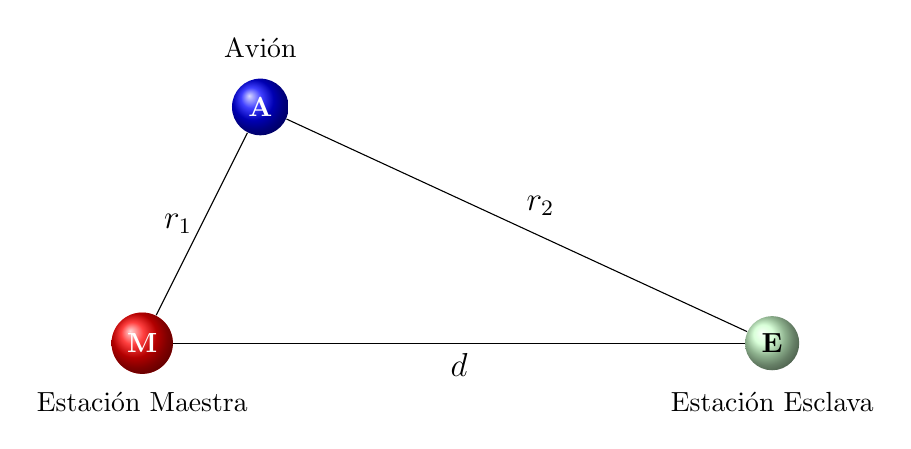
\begin{tikzpicture}[scale=1]
\usetikzlibrary{snakes}
\usetikzlibrary{calc}

%  \draw[help lines, green!70, step=0.5] (0,0) grid (9,4);
	% Impulso tiempo t0

	\node[circle, 
				shading=ball, 
				fill=red!50, 
				ball color=red,
				text=white
				] (M) at (0,0) {$\bf M$};

	\node[circle,
				shading=ball, 
				ball color=green!20,
%				text=white
				] (E) at (8,0) {$\bf E$};

	\node[circle,
				shading=ball,
%				ball color=black,
				text=white
				] (A) at (1.5,3) {$\bf A$};

	\draw (M) ++(0.0,-0.5) node[anchor=north] {Estaci\'on Maestra}; 
	\draw (E) ++(0.0,-0.5) node[anchor=north] {Estaci\'on Esclava}; 
	\draw (A) ++(0.0,1.0) node[anchor=north] {Avi\'on}; 

	\draw (M) -- (A) node[midway, above,anchor=east] {\large $r_1$};
	\draw (E) -- (A) node[midway, above,anchor=south west] {\large $r_2$};
	\draw (M) -- (E) node[midway, above,anchor=north] {\large $d$};

\end{tikzpicture}
\end{wrapfigure}

Pero la ecuaci\'on encierra una gran dificultad de llevar a la pr\'actica puesto que $t_0$ implica conocer el momento exacto en que se produjo la transmisi\'on del emisor. Este problema desaparece si se considera, en lugar de una distancia determinada a una estaci\'on, una diferencia de distancias a dos estaciones puesto que si ambas transmiten sincronizadas, al efectuarse la diferencia de distancia la inc\'onita $t_0$ desaparece.

Para ver con mas detalle lo anterior, consid\'erese una estaci\'on emisora maestra, $M$  que empieza su emisi\'on en el tiempo $t_0$; otra estaci\'on denominada esclava ubicada a una distancia $d$ de la estaci\'on maestra, recibe esta se\~nal luego de un tiempo $d/c$. Luego de un tiempo $\tau$, denominado ``tiempo de sincronismo'', emite una se\~nal id\'entica a la recibida. 

El receptor en la aeronave ($A$) recibe las se\~nales emitidas por las emisoras maestra y esclava, calculando la diferencia de tiempo entre ambas $\Delta\,t = t_2-t_1$. 

Partiendo de la estaci\'on maestra en el tiempo $t_0$, el impulso tarda un tiempo $t_1-t_0$ en llegar al receptor de la aeronave:

\[t_1-t_0 = \displaystyle \frac{r_1}{c}
\]

Al llegar el impulso de la estaci\'on madre a la esclava, esta luego del tiempo $\tau$, emite el suyo el cual llega en el tiempo $t_2$ al receptor, de esta forma se tiene:

\[
t_2-t_0 = \displaystyle \frac{d}{c}+\tau+\frac{r_2}{c}
\]

Haciendo la diferencia de $t_2-t_1$ seg\'un las expresiones anteriores:

\[
t_2-t_1 = t_0 + \displaystyle \frac{d}{c}+\tau+\frac{r_2}{c} - t_0 -\frac{r_1}{c} = \tau+\frac{d+r_2-r_1}{c} = \tau+\frac{d+\Delta\,r}{c}
\]

Finalmente:

\[
\Delta\,t = \tau+\frac{d+\Delta\,r}{c}
\]

Esta expresi\'on implica que a cada incremento de tiempo ($\Delta t$) le corresponde uno de distancia ($\Delta r$), con los par\'ametros $d$, $c$ y $\tau$ conocidos.

Pero debe recordarse algo, en lugar de considerar hip\'erbolas que son curvas planas, este m\'etodo ubica al receptor en un hiperboloide de revoluci\'on. Por esto deben hacerse correcciones por la curvatura y forma de la tierra.


\item [T\'ecnica de onda continua-fases:]

En esta t\'ecnica la emisi\'on es de forma continua a diferencia de la anterior que es por pulsos y que el par\'ametro que se mide es la diferencia de fases.

Se utilizan dos emisores omnidireccionales con un sincronismo de fases entre sus se\~nales. El receptor recibe a ambas se\~nales con una diferencia de fase, que depende de la distancia de la aeronave a cada una de las emisoras. De esta manera se determina la hip\'erbola donde se encuentra el receptor.

Conociendo la longitud de onda $\lambda$ se puede obtener la distancia recorrida seg\'un la fase medida: 

\[\Delta r = \lambda \,\Delta \phi \quad \Longrightarrow r = r_0 +\lambda \,\left( \phi - \phi_0 \right) \]

Aqui se presenta una dificultad porque el receptor necesita conocer $ \phi_0$, la fase exacta en que se produjo la transmisi\'on.

El proceso se realiza de la siguiente forma, la estaci\'on maestra ubicada en $M$ emite su se\~nal continua con frecuencia $f_1$ (longitud de onda $\lambda_1$) y origen de fases $ {\phi_1}_0$. La estaci\'on esclava en $E$ recibe esta se\~nal y transmite la suya con frecuencia $f_2$ y fase inicial $ {\phi_2}_0$. La frecuencia $f_2$ es diferente de la $f_1$ para que el receptor pueda separar facilmente las se\~nales.

La antena de la aeronave recibe ambas se\~nales $f_1$ y $f_2$ con fases $\phi_1$ y $\phi_2$ diferentes a las de salida, cuyos valores son:

\[
\phi_1 = {\phi_1}_0 + \displaystyle \frac{r_1}{\lambda_1} \qquad
\phi_2 = {\phi_2}_0 + \displaystyle \frac{r_2}{\lambda_2} 
\]

Para poder comparar estas se\~nales se usa el artificio de una frecuencia com\'un, $f_c$, con longitud de onda $\lambda_c$ que resulta de multiplicar a cada una de las frecuencias anteriores por un n\'umero entero $n_1$ y $n_2$, respectivamente:

\[
f_c = n_1\,f_1 = n_2\,f_2
\]

Cuando se multiplica una frecuencia por un n\'umero, se hace lo mismo con su fase, por lo que las expresiones anteriores vistas desde esta frecuencia com\'un, quedan:

\[
\theta_1 = n_1\,\phi_1 = n_1\,{\phi_1}_0 + \displaystyle \frac{n_1\,r_1}{\lambda_1} \qquad
\theta_2 = n_2\,\phi_2 = n_2\,{\phi_2}_0 + \displaystyle \frac{n_2\,r_2}{\lambda_2} 
\]

Restando la diferencia de las fases:

\[
\Delta\,\theta = \theta_1-\theta_2 = n_1\,{\phi_1}_0 + \displaystyle \frac{n_1\,r_1}{\lambda_1} -  n_2\,{\phi_2}_0 - \displaystyle \frac{n_2\,r_2}{\lambda_2} 
\]

El sincronismo de fase entre la estaci\'on maestra y la esclava debe realizarse de forma que se cumpla lo siguiente:

\begin{itemize}
\item La diferencia de fases iniciales multiplicadas por su entero respectivo debe mantenerse constante: $n_1\,{\phi_1}_0- n_2\,{\phi_2}_0= cte$

\item El ajuste de sincronismo que realiza la estaci\'on esclava cumple, en la prolongaci\'on de la l\'inea que la une con la maestra pero en el lado de la maestra, que la diferencia de fases en la aeronave sea nula: 

Para $r_1=0$ y $r_2=d$ se cumple que $\Delta\,\theta = \theta_1-\theta_2 =0$

\end{itemize}

Sabiendo que para un lado se cumple $c = f_c\,\lambda_c = f_1\,\lambda_1$ y como $f_c=n_1\,f_1$, entonces $n_1f_1\lambda_c = f_1\lambda_1$, por lo que $n_1\lambda_c=\lambda_1$ o $\displaystyle \frac{n_1}{\lambda_1}=\frac{1}{\lambda_c}$.

De la misma manera se obtiene $\displaystyle \frac{n_2}{\lambda_2}=\frac{1}{\lambda_c}$.

Volviendo a la diferencia de fases de la frecuencia com\'un:

\[
\Delta\,\theta = n_1\,{\phi_1}_0- n_2\,{\phi_2}_0 +  \displaystyle \frac{n_1\,r_1}{\lambda_1}  - \displaystyle \frac{n_2\,r_2}{\lambda_2}= cte + \frac{\Delta r}{\lambda_c}
\]

Trabajando con la expresi\'on anterior se llega a que:

\[
\Delta \theta = \displaystyle \frac{d+\Delta r}{\lambda_c}
\]

Surge un problema adicional, esta expresi\'on solo resuelve el incremento de fase dentro de una longitud de onda determinada pero se desconoce dentro de cual. 
Esto resulta en una indeterminaci\'on m\'ultiple, ya que el \'angulo real ser\'a un n\'umero entero de longitudes de onda m\'as el desfase obtenido de la ecuaci\'on anterior. 
La indeterminaci\'on ser\'a mayor cuanto mayor sea la frecuencia de la se\~nal radiada (menor $\lambda$). 
El inconveniente se soluciona con otra t\'ecnica conocida como del n\'umero de longitudes de onda completas.


\end{description}


\subsection{LORAN}


El \textbf{LORAN} (del ingl\'es LOng RAnge Navigation, navegaci\'on de largo alcance) es un sistema de ayuda a la navegaci\'on electr\'onica de tipo hiperb\'olico
 de largo alcance, que opera en baja y media frecuencia. 

Utiliza el intervalo transcurrido entre la recepci\'on de se\~nales de radio transmitidas desde tres o m\'as transmisores para determinar la posici\'on del receptor. 

Desarrollado a principios de la II Guerra Mundial, el LORAN fue el primer sistema de navegaci\'on basado en la llegada diferenciada de se\~nales de radio. Fue concebido por el laboratorio de Radiaci\'on de MIT. LORAN fue, tambi\'en, el primer sistema de posicionamiento capaz de funcionar bajo cualquier condici\'on climatol\'ogica pero es solamente bidimensional (latitud y longitud).

\begin{figure}[!tbh]
  \centering
  \subfigure[Interior de la instalaci\'on emisora]{\includegraphics[height=5.5cm]{Imagenes/06.01.adf/LORAN-Equip-Hut_.jpg}}
  \subfigure[Vista de estaci\'on emisora]{\includegraphics[height=5.5cm]{Imagenes/06.01.adf/LORAN-A_1940-instalacion-terrestre.jpg}}
  \caption{Instalaciones de LORAN-A \cite{Historia_LORAN} }
\end{figure}

 El sistema emisor LORAN se compone de una estaci\'on maestra y otra esclava. La maestra emite de forma regular una peque\~na se\~nal, que es repetida por la esclava, controlada por radio desde la maestra. Ambas se\~nales se reciben en el barco o avi\'on, se amplifican y se registran como peque\~nas ondas sobre la pantalla de un tubo de rayos cat\'odicos. Los circuitos del receptor est\'an dispuestos de forma que la distancia entre las se\~nales corresponda a la diferencia de tiempos de llegada de las se\~nales de ambas estaciones. El receptor posee adem\'as un dispositivo temporizador electr\'onico que permite medir dicha diferencia en microsegundos (millon\'esimas de segundo).

Como las ondas de radio viajan a una velocidad aproximadamente constante de 300000 km/segundo, la ubicaci\'on de todos los puntos en los que las se\~nales de las dos estaciones est\'an separadas un determinado intervalo de tiempo se puede representar mediante una curva concreta que es una hip\'erbola (Figura \ref{fig:LORAN_hiperbolas}). El navegante dispone de un mapa con muchas de estas curvas, denominadas curvas de posici\'on LORAN, y tras determinar la diferencia de tiempos, por ejemplo, 3 microsegundos, sabe que la posici\'on de su nave se halla en alg\'un punto de la curva de 3 microsegundos del mapa. Sintonizando una pareja de emisores LORAN y repitiendo este proceso, el navegante es capaz de detectar otra curva que represente la posici\'on de la nave; la posici\'on real del aparato se halla en la intersecci\'on de las dos curvas LORAN. 


\begin{figure}[!tbh]
  \centering
  \includegraphics[width=0.95\textwidth]{Imagenes/06.01.adf/hypnavig.pdf}
  \caption{Mapa de hip\'erbolas del sistema LORAN \cite{Loran_conicas}}
  \label{fig:LORAN_hiperbolas}
\end{figure}


Este sistema posee un alcance \'util de unos 2592,8 km (1400 nm) por la noche y unos 1296,4 km (700 nm) de d\'ia. Las se\~nales se emiten generalmente en la banda de frecuencias de 1,8 a 2,0 MHz. Sirve tanto para marcar y mantener un rumbo, como para fijar la posici\'on, y presenta la ventaja de ser independiente de las condiciones meteorol\'ogicas. Su exactitud oscila entre unos centenares de metros y unos pocos kil\'ometros, dependiendo del equipo utilizado y de la distancia entre la nave y la emisora. 


La versi\'on m\'as moderna es LORAN-C que funciona en frecuencias del espectro electromagn\'etico entre 90 y 100 Khz. El sistema LORAN es utilizado en muchos pa\'ises, entre ellos los Estados Unidos de Am\'erica, Jap\'on y varios pa\'ises europeos. Rusia utiliza un sistema casi id\'entico llamado CHAYKA, que usa la misma banda de frecuencias. 

El uso de LORAN est\'a decayendo r\'apidamente siendo reeplazado por GPS. Sin embargo, se est\'a estudiando la posibilidad de mejorar y volver a popularizar el LORAN.

\begin{figure}[!tbh]
  \centering
    \includegraphics[width=\textwidth]{Imagenes/06.01.adf/Loran_A_Coverage_1973.jpg}
  \caption{Cobertura LORAN-A A\~no 1973 \cite{loran-history-info}}
  \label{fig:LORAN-A-cobertura-1973}
\end{figure}

\subsection{DECCA}

El sistema de navegaci\'on DECCA es un sistema hiperb\'olico de posicionamiento basado en se\~nales de radio de onda continua en el rango de frecuencias de los 70 a los 130 Khz. Su uso puede aplicarse tanto en entornos mar\'itimos, a\'ereos y terrestres. El sistema consta de estaciones emisoras en tierra situadas en localizaciones conocidas que crean l\'ineas de posici\'on hiperb\'olicas. El alcance del sistema depende de varios factores pero normalmente es del orden de 240 millas mar\'itimas (unos 440 Km) durante la noche y el doble de esta distancia por el d\'ia. Una cadena de estaciones DECCA consta de una estaci\'on central Master, a la que se asocian las tareas de supervisi\'on, control y monitorizaci\'on de la cadena, junto con tres, en algunos casos dos, estaciones esclavas alejadas a unos 80-110 Km. de la Master.

Inventado en Am\'erica por Wiilian J.O'Brien, pero desarrollado por la empresa londinense ``DECCA Radio and Televisi\'on, Ltd.'',el sistema DECCA se us\'o inicialmente para dirigir el rumbo de los dragaminas durante el desembarco de Normand\'ia en la Segunda Guerra Mundial. El DECCA comenz\'o a transmitir el 5 de junio de 1944. En 1975, Mr H. Schwarz, el director general de la Compa\~nia DECCA Navigator, admiti\'o que el Loran-C era probablemente mejor que el DECCA en navegaci\'on a\'erea y que la navegaci\'on por sat\'elite era posiblemente mejor que ambos. Ante la competencia del sistema GPS, DECCA suspendi\'o su servicio entre los a\~nos 2000 y 2001.\cite{wikipedia_esp}

\subsubsection{ Funcionamiento}


Para poder determinar exactamente la posici\'on de un m\'ovil en el espacio el Sistema DECCA necesita usar al menos tres estaciones transmisoras en tierra. Este conjunto de estaciones transmisoras son lo que conocemos como ``Cadena DECCA''.

Cada cadena dispone de una estaci\'on Master y de tres, en algunos casos dos, estaciones Esclavas, a las que se denominan correspondientemente con los nombres de Roja, Verde y P\'urpura. Entre la estaci\'on Master y cada estaci\'on Esclava se crea un haz iperb\'olico que es la representaci\'on gr\'afica de las diferencias de fase existentes entre las emisiones de cada par de estaciones transmisoras.De este modo un aparato Receptor que reciba las emisiones de las estaciones puede hallar y mostrar de forma exacta la posici\'on de cualquier m\'ovil en un momento determinado, ya que la posici\'on ser\'a el punto de intersecci\'on de, al menos, un par de hip\'erbolas.

Para que esto suceda primero debemos crear un patr\'on o haz hiperb\'olico entre la estaci\'on Master y cada una de las Esclavas.

El sistema hace uso de frecuencias diferentes para cada una de las estaciones transmisoras, pero todas ellas est\'an arm\'onicamente relacionadas (son proporcionales), es lo que conocemos como arm\'onicos.

Toda Cadena DECCA dispone de una frecuencia fundamental no modulada que no es transmitida conocida como \textbf{f}. Est\'a frecuencia se encuentra en la banda de los 14 kHz. La estaci\'on Master transmite a 6f, la Esclava P\'urpura a 5f ,la Esclava Roja emite a 8f y la Esclava Verde lo hace a 9f .Al ser se\~nales de onda continua es suficiente espaciarlas 180Hz para evitar interferencias.

Para crear el patr\'on o haz hiperb\'olico entre un par Master-Esclava la estaciones deben estar sincronizadas en fase y en frecuencia.

Aunque las estaciones no emiten a la misma frecuencia (el Receptor no ser\'ia capaz de distinguir entre las se\~nales de las Esclavas y de la Master), todas emiten en m\'ultiplos de la frecuencia fundamental. Para crear el patr\'on o haz hiperb\'olico necesitamos que las ondas emitidas sean de la misma frecuencia, esto lo conseguimos “virtualmente” en el Receptor ya que despu\'es de multiplicar convenientemente cada frecuencia, se comparan siempre a una misma frecuencia final (24f para el par Master–Roja, 18f para el par Master–Verde y 30f para el par Master–P\'urpura). El resultado final es que el Receptor calcula las diferencias de fase como si cada estaci\'on emitiese a la misma frecuencia.

Una vez creado el patr\'on o haz de hip\'erbolas en cada par Master-Esclava el Receptor DECCA puede determinar la posici\'on al comparar la diferencia de fases entre cada par Master y Esclava. Las diferencias de fase medidas en el Receptor se representan en los dec\'ometros. Las lecturas de los dec\'ometros son trasladadas manualmente a una Carta de navegaci\'on DECCA donde est\'an representadas gr\'aficamente las hip\'erbolas, cada una con su color correspondiente (Rojo, Verde y P\'urpura). El punto de intersecci\'on de al menos dos hip\'erbolas (tres para conseguir mayor exactitud) nos da nuestra posici\'on.

Un Receptor DECCA en su versi\'on m\'as simple se presenta en la Figura . En el diagrama de bloques podemos ver los filtros, multiplicadores y discriminadores que hacen posible las lecturas de los dec\'ometros. Los Receptores filtran la se\~nal procedente de cada Esclava y de la Master. Estas se\~nales son multiplicadas convenientemente para poder compararlas a la misma frecuencia en los discriminadores (virtualmente es como si las estaciones emitiesen a la misma frecuencia). Estos c\'alculos son los que se representan en los dec\'ometros.

\begin{figure}[!h]
  \centering
  \includegraphics[width=0.8\textwidth]{Imagenes/06.01.adf/receptor_decca.gif}
  \caption{Diagrama de Bloques de un receptor DECCA en su versi\'on m\'as simple (sin indicador de calle). La se\~nal de cada estaci\'on Esclava y de la Master es captada, filtrada y multiplicada para poder hacer la comparaci\'on de fase en los discriminadores a una misma frecuencia. Los calculos realizados en los discriminadores se representan finalmente en los dec\'ometros.}
  \label{fig:DECCA-receptor}
\end{figure}

\begin{figure}[!h]
  \centering
  \includegraphics[width=0.6\textwidth]{Imagenes/06.01.adf/DECCA-0002.jpg}
  \caption{Receptor DECCA}
  \label{fig:DECCA-receptor-2}
\end{figure}

Para calcular la diferencia de fase, y por tanto la l\'inea de posici\'on, el Receptor hace uso de la siguiente f\'ormula:

\[
\Delta \phi =\displaystyle  \frac{2\pi\left(S+r\,a-r\,b\right)}{\lambda}
\]

Donde se considera que A y B son un par de estaciones transmitiendo sincronizadamente que emiten ondas continuas de id\'entica frecuencia y fase.

\begin{itemize}
\item $r\,a(r\,b)$ es la distancia a la estaci\'on A(B).

\item $\lambda$ es la longitud de onda de la frecuencia com\'un.


\item $S$ es la distancia entre las dos estaciones.
\end{itemize}


El lugar de los puntos de un plano en el que $rA-rB$ es una constante se representa gr\'aficamente mediante una hip\'erbola de focos A y B. Lo que constituye una l\'inea de posici\'on para la navegaci\'on si la localizaci\'on de las estaciones es conocida y el usuario dispone de un equipo comparador de fase.

\begin{figure}[!htb]
  \centering
  \includegraphics[width=0.6\textwidth]{Imagenes/06.01.adf/receptor_decca_multipulso.gif}  
  \caption{Diagrama de Bloques de un receptor DECCA preparado para el Multipulso (Indicador de Calle). Las emisiones de todas las estaciones se suman en el creador del Multipulso consiguiendo una forma de onda que tiene como caracter\'istica dominante un corto impulso redundante de frecuencia f. Durante la transmisi\'on Multipulso (MP) de la Master el receptor memoriza la fase de la transmisi\'on y la compara dando como resultado 0. En las dem\'as emisiones se compara la fase del MP de cada estaci\'on con la fase MP memorizada de la Master, creandose as\'ii un haz o patr\'on hiperb\'olico que por cada ciclo de diferencia de fase agrupa a 18 calles verdes, 24 rojas y 30 p\'urpuras. Las diferencias de fase se representan en el Indicador de Calle.}
  \label{fig:receptor-decca-multipulso}
\end{figure}

El medidor de fase o dec\'ometro no puede distinguir diferencias de fase m\'ultiplos de $2\pi$ (360º) por eso el rotor del dec\'ometro (que realiza un giro completo por cada 360º de fase) esta conectado mediante un engranaje a la aguja principal que avanza una posici\'on cada vez se recorre el espacio comprendido entre dos hip\'erbolas en fase. Por convencionalismo el rotor del dec\'ometro avanza en el sentido de las agujas del reloj en direcci\'on hacia la Esclava. El espacio comprendido entre dos hip\'erbolas en fase se denomina Calle o ruta DECCA (DECCA Lane). Conectado al rotor de calle hay otro rotor calibrado en cent\'esimas de calle. En la pr\'actica una carta DECCA consta de varios cientos de calles que se agrupan en Zonas designadas alfab\'eticamente por letras de la A a la J.


\begin{figure}[!htb]
  \centering
  \includegraphics[width=\textwidth]{Imagenes/06.01.adf/DECCA-carta-simplificada.gif}  
  \caption{
Carta DECCA Simplificada en la que se representa como las lecturas de un par de dec\'ometros nos indican nuestra posici\'on.
}
  \label{fig:Decca-carta-simplificada}
\end{figure}


\begin{figure}[!htb]
  \centering
  \includegraphics[width=\textwidth]{Imagenes/06.01.adf/DECCA-secuencia-transmision.gif}  
  \caption{Secuencia de transmisi\'on de 20 segundos de una Cadena DECCA Multipulso. De los 0,15s a los 1,60s podemos observar como la Master emite todas las frecuencias (Multipulso Master). El multipulso de la Roja es de los 2,65s a los 3,10s, el de la Verde de los 5,15 a los 5,60 segundos y el P\'urpura de los 7,65s a los 8,10s. Las emisiones Naranjas son del tipo 8.2f. Las naranjas con franjas negras (8.2f) son transmisiones de comandos y datos para control y supervisi\'on de la cadena. }
  \label{fig:DECCA-secuencia-transmision}
\end{figure}

La antena tranmisora es normalmente una torre de 100 metros. La potencia del transmisor era de $1.2$\,kW a cada frecuencia, pero dada la corta longitud de la antena en comparacion con longitud de onda, la potencia radiada era de 100 a 200 W.

La exactitud del sistema DECCA depende en gran medida de la posicion del usuario con respecto a las estaciones transmisoras, asi como de la \'epoca del a\~no y de la hora del d\'ia. La desviaci\'on est\'andar del error en el DECCA se med\'ia habitualmente en cent\'esimas de calle. Los errores de d\'ia oscilaban entre unos pocos de metros, por contra de noche los errores eran mayores llegando hasta millas. En cuanto al alcance de las estaciones transmisoras, era de 740km por el d\'ia y 460 durante la noche. El alcance se suele definir como la distancia a la cual las reflexiones de la ionosfera alcanzan el mismo nivel de intensidad que la onda de superficie. 

El uso de un receptor DECCA en la cercan\'ia de la costa era una fuente de errores debido a la presencia de monta\~nas, puentes o l\'ineas de alta potencia, que pod\'ian provocar reflexiones que hacen que el camino de propagaci\'on no sea el m\'as corto.

\newpage

\section{ADF}

\subsection{Introducci\'on}
\label{sec:adf.introduccion}

\begin{itemize}
\item El ADF (Automatic Direction Finder), es uno de los sistemas de
  radio navegación mas antiguos, est\'a compuesto por un equipo
  llevado a bordo de la aeronave y otros en tierra.

\item   La funci\'on del ADF es indicar al piloto la direcci\'on en la cual
  se encuentra una radioayuda NDB (o radioemisora) dada.

\item   La NDB (Non-Directional Beacon) es la correspondiente radioayuda en
  tierra que se sintoniza, mientras que el ADF es el equipo a bordo de
  la aeronave. El ADF puede utilizar se\~nales de otras fuentes, como
  radioemisoras comerciales.

\item   A nivel mundial, se utiliza el ancho de banda entre 200 kHz y 1750
  kHz (aunque los l\'imites pueden variar un poco seg\'un el
  lugar). En Europa los NDB t\'ipicamente se encuentran en las
  sub-bandas 255-415 y 510-525 kHz.

\item   Este rango de frecuencias coloca al sistema en el reino de la MF
  (Medium Frecuencies), existiendo ondas ionosf\'ericas (o de cielo) y
  ondas de tierra. Estas \'ultimas son capaces de llegar a largas
  distancias y sobrepasar obst\'aculos.

\item   Correspondientemente, la longitud de onda es bastante grande
  comparada con las dimensiones de una aeronave: f = 200 kHz -
  $\lambda = 1500$ m, y f = 1750 kHz - $\lambda = 171.429$ m.

\item   La se\~nal se emite en AM (amplitud modulada),envi\'andose la
  identificaci\'on de la estaci\'on en c\'odigo Morse (para los NDB) o
  m\'usica y sonidos en el caso de las radioemisoras comerciales.

\item   El alcance es de 25 a 100 NM (46,3 a 185,2 km), puede ser mayor,
  pero aparecen problemas.

\item   La intensidad de campo requerida es de 70 microVoltios/m, con S/N >
  15 dB.

\item   La precisi\'on media obtenida es de 3 a 5 grados en condiciones
  normales de operaci\'on.

\item   La polarizaci\'on es vertical (campo el\'ectrico en la direcci\'on
  ``z''), con propagaci\'on horizontal.
\end{itemize}


\subsection{Antena de cuadro}


La antena de cuadro (tambi\'en llamada antena loop), es una evoluci\'on de las antenas ``Adcock'' que consiste en dos antenas verticales aisladas conectadas en contrafase, ver Figura \ref{fig:antena.adcock}.

La antena de cuadro tiene las antenas verticales conectadas entre s\'i y est\'a hecha de varias vueltas de hilo conductor para mejorar sus propiedades de recepci\'on, como se muestra en la Figura \ref{fig:antena_cuadro}.

Las dos secciones verticales de la antena son las que reciben se\~nal, son paralelas entre s\'i y est\'an conectadas en ``contrafase'', lo que significa que lo que reciben se resta entre s\'i y lo que sale es la diferencia.

\begin{figure}[!htb]
  \centering
 \subfigure[Antena Adcock %\\ {\tiny Fuente:\url{http://www.flyingstart.ca/FlightTraining/preflight/antennae.html}}
	]{
	 \includegraphics[height=6.5cm]{Imagenes/06.01.adf/adcock-antena-01.jpg}
	 \label{fig:antena.adcock}
	 }
% \subfigure[Antigua antena de cuadro ubicada en la parte baja del fuselaje de un DC3.\\ {\tiny Fuente:armyintelligence.tpub.com/IT0302/IT03020036.htm}]{\includegraphics[height=6.5cm]{Imagenes/06.01.adf/DC3-loop-antena.jpg}  \label{fig:antena.loop.vieja}}
 \subfigure[Antigua antena de cuadro ubicada en la parte baja del fuselaje de un DC3]{\includegraphics[height=6.5cm]{Imagenes/06.01.adf/DC3-loop-antena.jpg}  \label{fig:antena.loop.vieja}}
  \caption{Antenas}
\end{figure}



\subsection{Radiogoni\'ometro}

La evoluci\'on del ADF ha sido en fases. La primera de ellas fue el radiogoni\'ometro, que hallaba la direcci\'on en la cual se encontraba una estaci\'on emisora en tierra, pero NO lo hac\'ia de manera autom\'atica.

Este instrumento ten\'ia una antena de cuadro que pod\'ia girarse manualmente desde la cabina, como la mostrada en la Figura \ref{fig:antena.loop.vieja}.

El siguiente dibujo representa una antena de cuadro cuyo plano est\'a inclinado un cierto \'angulo $\theta$ con respecto al origen de la se\~nal:


\begin{figure}[!h]
  \centering
\subfigure[Antena de cuadro \cite{ADF-teoria}]{  \includegraphics[width=0.3\textwidth]{Imagenes/06.01.adf/antena-cuadro.png}  \label{fig:antena_cuadro}}
\subfigure[Recepci\'on de la se\~nal por la antena de cuadro \cite{ADF-teoria}]{  \includegraphics[width=0.6\textwidth]{Imagenes/06.01.adf/antena-cuadro-recibiendo-senial.png}  \label{fig:antena_cuadro_recibiendo_senial}}
  \caption{Antena de cuadro}
\end{figure}


En la Figura \ref{fig:antena_cuadro_recibiendo_senial} se puede apreciar claramente que debido a que la ``Antena 1'' (Ant. 1 en la figura) y la ``Antena 2'' (Ant. 2) est\'an separadas una cierta distancia y, adem\'as, existe un \'angulo entre la se\~nal que llega y el plano que une las antenas ($\theta$), la primera recibe la se\~nal antes que la segunda. Por esto existe un desfase entre ambas, y por tanto una diferencia (la salida de la antena de cuadro NO es cero en este caso).

 En la Figura \ref{fig:seniales-recibidas-antena-cuadro} se ilustra la forma de las se\~nales recibidas por la antena 1 ($y_1$), la antena 2 ($y_2$) y la diferencia entre ellas ( $y_3 = y_2 - y_1$ ), que es realmente la salida de la antena de cuadro.

\begin{figure}[!h]
  \centering
  \subfigure[Se\~nales recibidas por la antena de cuadro ]{  \includegraphics[, height=6cm]{Imagenes/06.01.adf/adf-seniales-antena-cuadro.eps}  \label{fig:seniales-recibidas-antena-cuadro}}
  \subfigure[Se\~nales recibidas por la antena de cuadro ]{  \includegraphics[height=6cm]{Imagenes/06.01.adf/diagrama-recepcion-antena-cuadro.png}  \label{fig:diagrama-recepcion-antena-cuadro}}

  \caption{Esquemas funcionamiento antena de cuadro}
\end{figure}

En la Figura \ref{fig:diagrama-recepcion-antena-cuadro} se muestra un diagrama de recepci\'on de estas antenas, el resultado es una figura de ``ocho'', donde la recepci\'on es mayor cuando la se\~nal llega paralela al plano de la antena de cuadro, y nula cuando viene perpendicularmente.


Esta caracter\'istica es aprovechada para hallar la direcci\'on de donde proviene la se\~nal. El ``radionavegante'' a bordo del avi\'on ten\'ia en su panel de control una ruedecilla (acoplada a un indicador de direcci\'on) con la que pod\'ia girar a voluntad (y manualmente) la antena de cuadro, mientras simult\'aneamente escuchaba con sus aud\'ifonos la se\~nal de audio proveniente del emisor (NDB o estaci\'on de radio comercial).

Cuando el radionavegante dejaba de escuchar la se\~nal significaba que el plano de la antena de cuadro estaba perpendicular a la direcci\'on en la cual se encontraba el emisor, tomando nota de dicha direcci\'on (mostrada en el indicador) y marc\'andola en su carta de navegaci\'on.

El m\'etodo anterior encuentra la direcci\'on pero \emph{existe una ambigüedad en el sentido}, pues el emisor puede estar a un lado u otro del plano de la antena de cuadro. Esta ambigüedad era resuelta tomando otros emisores como referencia, y hayando la intersecci\'on de las direcciones, o llevando un registro cuidadoso de la trayectoria del avi\'on desde el inicio del vuelo.

En la Figura \ref{fig:diag-bloques-radiogoniometro} se ilustra el diagrama de bloques del radiogoni\'ometro.


\begin{figure}[!h]
  \centering
   \includegraphics[width=0.6\textwidth]{Imagenes/06.01.adf/diag-bloques-radiogoniometro.png}
  \caption{Diagrama de bloques del radiogoni\'ometro}
  \label{fig:diag-bloques-radiogoniometro}
\end{figure}


En un circuito aparte, alimentado por una ``\emph{antena de referencia}'', proporciona una se\~nal en el sistema de audio que no est\'a sometida a las variaciones de amplitud que implica el cambio de direcci\'on de la antena de cuadro.


\subsection{ADF}

La diferencia principal entre el radiogoni\'ometro y el ADF es que este \'ultimo es \emph{autom\'atico}, como lo indica su nombre. Esto indica que la ambigüedad en el sentido debe resolverse dentro del propio equipo.

Para ello, se instala una antena de referencia que, por comodidad, se representar\'a en el centro de la antena de cuadro. La se\~nal recibida por esta antena se considera que no tiene desfase y al graficarla en el tiempo ($y_4$) estar\'a entre $y_1$ y $y_2$.


\begin{figure}[!h]
  \centering
  \subfigure[Se\~nales recibidas por la antena de cuadro + se\~nal de referencia. ]{  \includegraphics[width=0.45\textwidth]{Imagenes/06.01.adf/adf-+seniales-antena-cuadro.eps}  \label{fig:seniales-2}}
  \subfigure[Se\~nales antena de cuadro + referencia + referencia desfasada 90º. ]{  \includegraphics[width=0.45\textwidth]{Imagenes/06.01.adf/senyales-3.png}  \label{fig:seniales-3}}

  \subfigure[Diagrama de recepci\'on antena de cuadro + antena de referencia.]{  \includegraphics[width=0.65\textwidth]{Imagenes/06.01.adf/diag-recepcion-2.png}  \label{fig:diag-recepcion-2}}

  \caption{Se\~nales recibidas por la antena de cuadro}
\end{figure}



Si la se\~nal de referencia se desfasa 90º (ver curva $y_5$), podemos apreciar que pr\'acticamente entra en fase con $y_3$, que es la salida de la antena de cuadro cuando la antena 1 est\'a m\'as cerca del emisor que la antena 2. Correspondientemente, $y_5$ estar\'a en contrafase con $y_3$ si es la antena 2 la que est\'a m\'as cerca del emisor ($y_6 = y_1 - y_2$). Lo anterior se representa en la Figura \ref{fig:seniales-3}. 

Esta caracter\'istica de la recepci\'on se aprovecha para determinar el sentido en el que se encuentra el sector y as\'i resolver la ambigüedad que padec\'ia el radiogoni\'ometro. Si se hace un diagrama de recepci\'on de la combinaci\'on antena de cuadro + antena de referencia, se obtiene una \emph{cardioide}.


Entonces, la se\~nal de la antena de cuadro es introducida alternativamente a dos combinadores que generan 2 cardioides: Uno recibe $y_3$ ($y_2-y_1$) y el otro $y_6$ ($y_1-y_2$). \'Estos a su vez tambi\'en reciben $y_5$ y la salida de ambos alimenta a un comparador.

El resultado de la comparaci\'on es amplificado y alimenta a su vez al motor que mueve el cuadro. Este motor girar\'a en un sentido u otro seg\'un el signo de la comparaci\'on, dejando de mover la antena cuando la se\~nal de ambas cardioides es igual. Un acoplador "selsyn" conectado al motor del cuadro transmite la se\~nal hasta un indicador en la cabina de vuelo.

Esto se visualiza mejor con un diagrama de bloques del sistema presentado en la Figura \ref{fig:diag-bloques-adf-rot}.


\begin{figure}[!h]
  \centering
\subfigure[Diagrama de bloques del ADF con antena rotatoria]{ \includegraphics[width=0.75\textwidth]{Imagenes/06.01.adf/diag-bloques-adf-rot.png}   \label{fig:diag-bloques-adf-rot}}
\subfigure[Diagrama de bloques del ADF con antena rotatoria]{ \includegraphics[width=0.75\textwidth]{Imagenes/06.01.adf/esquema-adf-rot.png}   \label{fig:esquema-adf-rot}}
  \caption{}
\end{figure}


El siguiente esquema muestra las cardioides que el comparador est\'a recibiendo de los combinadores y c\'omo el sistema reacciona seg\'un cada caso, ver Figura \ref{fig:esquema-adf-rot}.

%\subsubsection{Reacciones del sistema ADF con antena rotatoria}

Para explicar estas reacciones vamos a estudiarlas por casos, siempre teniendo en cuenta que la flecha denotada como ``\emph{Sentido de la medida}'' representa la flecha del indicador:

\begin{description}
\item {Emisor en posici\'on A:} En este caso, la cardioide 1 (C1) es mayor que la cardioide 2 (C2), lo que hace que el comparador emita una se\~nal al motor del cuadro que har\'a rotar al conjunto COMO LAS AGUJAS DEL RELOJ (unos 150º en este caso) hasta que la flecha apunte hacia ``A''. Cuando se llegue a ese punto, $C_1=C_2$ y se detendr\'a el movimiento.


\item Emisor en posici\'on B: Ahora el comparador hallar\'a que C2>C1, y por tanto dar\'a al motor del cuadro la orden de giro AL CONTRARIO DE LAS AGUJAS DEL RELOJ hasta que la flecha apunte hacia "B", lugar en donde se detiene el giro porque C1=C2.
    

\item Emisor en posici\'on X: En este caso no hay movimiento porque la estaci\'on est\'a precisamente en donde C1=C2. No obstante, si por alguna desviaci\'on de la aeronave resulta que la flecha apuntara brevemente un poco "por debajo" de "X", entonces C1>C2 y el motor empezar\'a a girar como las agujas del reloj, lo que posicionar\'a la flecha otra vez en "X". Si por el contrario la flecha apuntara brevemente "por encima" de "X", entonces C2>C1 y el motor girar\'ia al rev\'es del reloj, volviendo a colocar la flecha apuntando a "X". En definitiva, esta posici\'on es de equilibrio estable.


\item Emisor en posici\'on C: Esta posici\'on representa aparentemente un problema porque la estaci\'on est\'a situada justamente al contrario de lo indicado por la flecha, pero como C1=C2 en teor\'ia la aguja permanecer\'ia en la posici\'on err\'onea. Sin embargo, la m\'as ligera desviaci\'on de esta posici\'on provocar\'ia que el conjunto diera una vuelta de 180º, colocando a la flecha en la posici\'on correcta. Por ejemplo, si C se mueve relativamente un poco hacia abajo de abajo de la posici\'on actual, C2>C1 y la antena se mover\'ia al contrario del reloj, aumentando a cada momento la diferencia entre C2 y C1, hasta que se d\'e una vuelta completa y se encuentre de nuevo el equilibrio, ahora con la flecha apuntando en el sentido correcto. Por tanto, la posici\'on "C" es de "equilibrio inestable" y no representa un problema en la pr\'actica.
 
\end{description}
    

Conforme evolucion\'o la tecnolog\'ia, se encontraron maneras de desarrollar un sistema ADF que resolviera la ambigüedad de sentido sin necesidad de rotar la antena de cuadro, mejor\'andose la confiabilidad del sistema.

Para ello, se utilizan dos antenas de cuadro colocadas ortogonalmente. La que tiene su plano a lo largo del eje longitudinal del avi\'on (adelante-atr\'as) es la "antena coseno", mientras aquella cuyo plano coincide con el eje transversal es la antena seno".

De esta manera se tienen dos diagramas de recepci\'on en "ocho", perpendiculares entre s\'i, que generar\'an sus respectivas cardioides al ser adecuadamente combinados con la se\~nal proveniente de la antena de referencia. Observe el siguiente diagrama:



De forma an\'aloga al caso del ADF con antena rotatoria, las se\~nales provenientes de las antenas de cuadro son combinadas con la se\~nal de la antena de referencia y alimentan alternativamente (con una frecuencia de alternancia de 100 Hz) a un comparador de fases. La salida de \'este son los valores de seno y coseno del \'angulo theta entre el eje longitudinal del avi\'on y la posici\'on de la estaci\'on.

Estas se\~nales seno-coseno alimentan a los indicadores (por ejemplo, un Indicador Radio-Magn\'etico o RMI), o a trav\'es de una interfaz ARINC 429 a un bus de datos digital.

A continuaci\'on se encuentra el diagrama de bloques t\'ipico de este sistema:

\begin{figure}[!htb]
  \centering
  \subfigure[Diagrama de las antenas de cuadro ortogonales]{\includegraphics[width=0.75\textwidth]{Imagenes/06.01.adf/esquema-adf-fijo.png}\label{fig:esquema-adf-fijo}}
  \subfigure[Diagrama de bloques del ADF con antenas fijas]{\includegraphics[width=0.75\textwidth]{Imagenes/06.01.adf/diag-bloques-adf-fijo.png}\label{fig:diag-bloques-adf-fijo}}
  \caption{ADF fijo}
\end{figure}

\subsubsection{NDB}
Como se indic\'o previamente, el NDB es la radioayuda en tierra que corresponde al ADF. Las sub-bandas de frecuencia usadas en Europa para los NDB t\'ipicamente se encuentran entre 255-415 y 510-525 kHz. Los NDB modulan en AM su identificaci\'on de estaci\'on en c\'odigo Morse, compuesta usualmente por tres letras.

\begin{figure}[!htb]
  \centering
  \subfigure[S\'imbolo NDB usado en cartas aeron\'auticas ]{\includegraphics[width=0.3\textwidth]{Imagenes/06.01.adf/NDB-simbolo.png}\label{fig:esquema-adf-fijo}} 
	\hspace{6mm}
  \subfigure[Emisor NDB en 49° 12.35' N, 2° 13.20' W. Callsign JW - 'Jersey West'. 329.0 kHz]{\includegraphics[width=0.45\textwidth]{Imagenes/06.01.adf/NDB-transmisor.jpg}\label{fig:diag-bloques-adf-fijo}}
  \caption{NDB}
\end{figure}


Estos radiofaros con emisi\'on omnidirecciona en azimut tienen la caracter\'istica que sus antenas no pueden radiar en su direcci\'on longitudinal, por lo cual justo por encima de los NDBs se forma un cono en el cual NO existe se\~nal.

Este cono, caracter\'istico tambi\'en de otras radioayudas, es llamado ``cono de silencio'', y su \'angulo de abertura puede tener, en el caso de los NDB, hasta 45º.

El alcance de los NDB puede ir desde unas 25 NM hasta m\'as de 100 NM, dependiendo de la potencia de emisi\'on. M\'as all\'a de las 100 NM empiezan a aparecer importantes errores.

\subsubsection{Errores ADF-NDB}

El sistema ADF/NDB tiene errores que t\'ipicamente oscilan entre los 3 y 5 grados. Hay dos tipos principales de error que son:

\begin{description}
\item [Errores Sistem\'aticos]

Los errores sistem\'aticos se pueden caracterizar previamente y tomar previsiones ante ellos. Los m\'as importantes son:

\begin{description}
\item [Error Instrumental]

Es el error asociado a incertidumbres en la lectura de los valores mostrados por los instrumentos. Oscila de 1 a 2 grados.

\item [Error por presencia del avi\'on]

La aeronave es un cuerpo met\'alico que puede interferir con la recepci\'on del sistema, distorsionando las se\~nales. Sin embargo, este error puede caracterizarse de f\'abrica y entonces tomar medidas correctivas.

\end{description}


\item [Errores Variables]

Como su nombre lo indica, son errores cuya aparici\'on y magnitud depende de m\'ultiples factores, siendo esencialmente desconocidos. Los m\'as conocidos son:

\begin{description}

\item [Errores atmosf\'ericos (tormentas)]

El n\'ucleo de las grandes tormentas genera poderosas cargas electromagn\'eticas cuya frecuencia puede estar en la banda de trabajo del ADF. Esto ocasiona que las tormentas puedan aparecer como estaciones en tierra y el ADF apuntar\'a hacia ellas. Es muy peligroso que el piloto las confunda con estaciones reales y vuele hacia ellas.


\item [Errores de polarizaci\'on]

Ciertas condiciones pueden alterar la polarizaci\'on y propagaci\'on de las se\~nales y ocasionar errores. Las m\'as conocidas son:

\begin{description}
\item [Efecto de l\'inea de costa], causado por la diferente conductividad entre la corteza terrestre y el agua, ocasionando que la se\~nal se refracte al pasar por la costa y genere indicaciones erradas.


\item [Efecto monta\~na], en donde debido a la orograf\'ia las ondas de tierra se pueden distorsionar, apareciendo errores de medici\'on.

\end{description}


\item [Interferencia xDSL (en estudio)]

La transmisi\'on de datos por Internet utilizando la tecnolog\'ia xDSL (HDSL, SDSL, VDSL y ADSL) puede generar se\~nales que interfieran con la operaci\'on del ADF y con las comunicaciones HF.

Debido a la naturaleza de los sistemas xDSL la fuente de interferencia est\'a distribuida geogr\'aficamente. Se est\'an realizando estudios para determinar si el efecto acumulativo de muchas de estas se\~nales puede alterar seriamente el funcionamiento del sistema (referencia actualizada al 21/Sep/2000).


\item [Efecto FADING]

Este efecto de ``desvanecimiento'' aparece porque a cierta distancia de la estaci\'on emisora las ``ondas de suelo'' y las ``ondas de cielo'' (estas \'ultimas por rebote ionosf\'erico) empiezan a interferir entre s\'i.

La interferencia entra ambas se\~nales puede ser constructiva o destructiva seg\'un el desfase que exista entre ellas, produci\'endose el efecto de una recepci\'on err\'atica e intermitente.

El siguiente gr\'afico representa la intensidad de campo versus la distancia a la estaci\'on, indicando las zonas en donde es m\'as probable que ocurra este efecto:

\begin{figure}[!htb]
  \centering
  \includegraphics[width=\textwidth]{Imagenes/06.01.adf/grafico-fading.png}
  \caption{ Gr\'afico del efecto ``fading''}
  \label{fig:fading}
\end{figure}

Una observaci\'on final es que durante la noche y cuando la aeronave se aproxima al ``terminator'' (l\'inea divisoria entre el d\'ia y la noche) es m\'as probable que se produzca este efecto, debido a la variaci\'on en la altura de la ionosfera.
\end{description}

\end{description}



%------------------VOR-----------------%

\chapter{VOR}
\label{sec:vor}

 %   % VOR
% version 2018
%-------------------------------------------------------

\section{Un poco de historia....}

\begin{wrapfigure}{r}{0.35\textwidth} \centering
  \includegraphics[keepaspectratio,width=0.3\textwidth]{Imagenes/06.02.vor.imagenes/Marconi.eps}\caption{Guillermo Marconi}
\end{wrapfigure}


Las radioayudas utilizadas actualmente (VOR, DME, ILS, etc.) se remontan a los primeros d\'ias de la radiocomunicaci\'on. Sus l\'ineas de origen se cruzan en muchos puntos, pero  encuentran, finalmente, su inicio en dos patentes registradas en Alemania en 1906.

Hacia 1905 Marconi hab\'ia dedicado un esfuerzo considerable a la investigaci\'on de las propiedades de la cl\'asica antena en L invertida. Encontr\'o que si el tramo horizontal era considerablemente mayor que el vertical, el diagrama polar presentaba un abombamiento considerable en la direcci\'on contraria a la l\'inea de secci\'on horizontal.

En 1905 patent\'o un sistema que utilizaba este tipo de antenas tanto para la emisi\'on como la recepci\'on, reivindicando excepcionales propiedades direccionales para la combinaci\'on. Bas\'andose en el mismo principio, Marconi registr\'o al a\~no siguiente la patente de un sistema con un n\'umero de antenas L invertidas igualmente espaciadas en forma radial alrededor del receptor. Seleccionando la antena que recib\'ia la se\~nal m\'as intensa pod\'ia averiguarse la direcci\'on aproximada de la estaci\'on emisora.

\begin{wrapfigure}{l}{0.35\textwidth}
  \centering  \includegraphics[keepaspectratio,width=\linewidth]{Imagenes/06.02.vor.imagenes/Telefunken.eps}
    \caption{La "br\'ujula"\, Telefunken} \label{fig:brujula.telefunken}
\end{wrapfigure}


Antes de que pasara un a\~no, Telefunken, en Alemania, hab\'ia introducido una idea muy parecida pero utilizando la parte emisora. Consist\'ia en un emisor que radiaba primero una se\~nal de inicio preestablecida a una antena central omnidireccional, seguida de una segunda emisi\'on en cada una de las 32 antenas espaciadas radialmente alrededor del radiador central omnidireccional y situadas seg\'un las marcaciones de la br\'ujula (Figura \ref{fig:brujula.telefunken}).

Una estaci\'on que desease utilizar la baliza, s\'olo ten\'ia que accionar un cron\'ometro al o\'ir la se\~nal de inicio y detenerlo cuando la se\~nal alcanzaba su m\'axima intensidad. Como ayuda a los usuarios del sistema se dise\~no un reloj especial. Ten\'ia una aguja que completaba una revoluci\'on en 32 segundos y su esfera estaba calibrada seg\'un los puntos de la br\'ujula.

Aunque este sistema no alcanz\'o nunca un uso generalizado, se le puede considerar como el precursor de todos los radiofaros giratorios modernos.

\begin{wrapfigure}{r}{0.35\textwidth} \centering
  \includegraphics[keepaspectratio,width=\linewidth]{Imagenes/06.02.vor.imagenes/bellinitosiprinciple.jpg}\caption{Principio del equipo de Bellini y Tosi}
\label{fig:bellini.y.tosi.principio}
\end{wrapfigure}

En 1907 Bellini y Tosi presentaron un dise\~no que comprend\'ia dos antenas receptoras de cuadro cruzadas a 90 grados a partir de las cuales se pod\'ia determinar la direcci\'on de las ondas incidentes, mediante la magnitud relativa de las corrientes que se induc\'ian en las antenas (Figura \ref{fig:bellini.y.tosi.principio}). Este sistema alcanz\'o un desarrollo ulterior y, durante la Primera Guerra Mundial (1914-1948), ambos contendientes depositaron una confianza considerable en el mismo. Pese a que una estaci\'on radiogonom\'etrica s\'olo pod\'ia controlar a un avi\'on a la vez y que, a veces, debido a desconocidos fen\'omenos de propagaci\'on, surg\'ian errores posicionales de mas de 50 millas; Von Buttlar-Brandenfels, el \'unico comandante de Zeppelin que vol\'o durante toda la guerra dedujo que la radionavegaci\'on era muy superior a la navegaci\'on astron\'omica.

\begin{figure}[!hbt]
  \centering  \includegraphics[keepaspectratio,width=0.8\textwidth]{Imagenes/06.02.vor.imagenes/Loran.eps}
    \caption{El sistema de aproximaci\'on de Lorenz.
	(a) Dispositivo de antenas. (b) Modelo de radiaci\'on. (c) Diagrama polar vertical y senda de aproximaci\'on.
}
    \label{fig:sistema.lorenz}
\end{figure}

A partir de 1916, Marconi inici\'o el estudio de radioenlaces direccionales de onda corta en una serie de experimentos que fueron llevados a cabo con diversas alternativas en Hendon y Cernavon, a partir de los cuales se desarroll\'o el ``\emph{faro de radioenlaces}'' que fue instalado en 1921 en Inchkeith Island. El hecho m\'as importante en el dise\~no de este equipo fue que \'unicamente pod\'ia generarse un haz suficientemente localizado como para proporcionar una exactitud digna de consideraci\'on, elevando la frecuencia al espectro de VHF. Adem\'as, el dise\~no de los sistemas de manipulaci\'on no permit\'ia que la baliza radiase informaci\'on err\'onea; asimismo el empleo del cron\'ometro se hizo innecesario.

Volviendo a 1907, una patente de O. Scheller de la compa\~n\'ia Lorenz, condujo a una l\'inea de desarrollo que, cuando se combin\'o con el radiofaro rotatorio de Marconi, culmin\'o con las radioayudas de hoy en d\'ia.

Era el ``Indicador de rumbo'', cuyo fundamento consist\'ia en que dos antenas con diagramas de radiaci\'on que se interceptaban, eran energizadas alternativamente por un \'unico transmisor. La potencia que se enviaba a una antena era utilizada para formar la letra ``A'' y la otra antena formaba la ``N''. La posici\'on de las antenas se dispon\'ia de tal manera que la intersecci\'on de sus diagramas de radiaci\'on correspondiese con el rumbo deseado. Por lo tanto, si una aeronave se encontrase fuera de rumbo, recibir\'ia una ``A'' o una  ``N'', pero si se encontrase en el rumbo, oir\'ia ambas simult\'aneamente, combin\'andose estas para dar un tono continuo.

En 1917 se realizaron experiencias en Alemania con barcos y cinco a\~nos m\'as tarde, Keibitz las realiz\'o con aviones. Aunque en tierra se hablaba de un margen de error de 30 m a 3,5 km de distancia, los resultados obtenidos fueron dudosos y la investigaci\'on qued\'o detenida hasta comienzos de la d\'ecada de 1930 cuando la compa\~n\'ia us\'o de nuevo el principio equise\~nal para su equipo de aproximaci\'on de VHF.

Este equipo de aproximaci\'on de Lorenz consist\'ia en un transmisor de VHF situado en la cabecera de la pista de aterrizaje y trabajaba a una frecuencia de aproximadamente 33 Mhz. Este sistema alimentaba un dipolo vertical a cuyos lados, formando \'angulo recto con la pista, se situaba un elemento reflector. El punto medio de cada uno de estos elementos reflectores estaba interrumpido y puenteado por
\begin{wrapfigure}{l}{0.45\textwidth} \centering
  \includegraphics[width=\linewidth]{Imagenes/06.02.vor.imagenes/Lorenz_beam.png}
%  \caption{\centering Se\~nales de Lorenz  \\{\tiny fuente: \url{http://en.wikipedia.org/wiki/Lorenz_beam }}} \label{fig:seniales.lorenz}
\end{wrapfigure}
un conjunto de contactos de rel\'e que operaban en oposici\'on, esto es, si un conjunto de contactos se encontraba cerrado el otro estar\'ia abierto, manteniendo sin funcionar ese reflector. Operando sobre los rel\'es, el diagrama de radiaci\'on pod\'ia ser trasladado de uno a otro lado. Ambos diagramas se interseccionaban sobre la l\'inea central de la pista  (Figura \ref{fig:sistema.lorenz}). La manipulaci\'on de los receptores se hac\'ia de modo que uno de ellos se manten\'ia en funcionamiento un per\'iodo de tiempo tres veces mayor que el otro; as\'i, cuando un piloto se aproximaba a la pista ligeramente fuera de rumbo, escuchaba una serie de ``E'' ($\cdot \, \cdot \, \cdot$) o de ``T'' ($- \, - \, -$) que se fund\'ian en un tono continuo ($- \cdot - \cdot - \cdot$) si se encontraba en el rumbo adecuado (Figura \ref{fig:seniales.lorenz}). Este sistema se denomin\'o \emph{Ultrakurzwellen-Landefunkfeuer} (LFF), o radiobaliza de ondas ultra-cortas para aterrizaje.


El receptor del avi\'on estaba dotado de un medidor de intensidad de se\~nal y pod\'ia obtenerse una gu\'ia de la senda de planeo siguiendo un contorno de igual intensidad de campo.

Este sistema se tambi\'en en Inglaterra con \'exito y se mantuvo en servicio hasta principios de 1960.

% \begin{figure}[!h]
%   \centering
%   \subfigure[Torre de control aeropuerto de Croydon (Inglaterra) coronada por los cuadros radiogonom\'etricos Bellini-Tosi {\tiny Fuente: \url{http://www.thecinetourist.net/the-hotel-bristol-enigma.html}}]{\includegraphics[height=6.0cm]{Imagenes/historia/croydon-control-tower-02.jpg}} 
%   \subfigure[Receptor radiogonom\'etrico Bellini-Tosi \\{\tiny Fuente: \url{http://www.airwaysmuseum.com/B-T\%20MFDF\%201.htm}}]{\includegraphics[height=6.0cm]{Imagenes/historia/bellini-tosi-medium-frecuency-direction-finder.jpg}}

%   \caption{Equipo de tierra sistema radiogoni\'ometro}
%   \label{fig:radiogoniometro}
% \end{figure}

En Estados Unidos se investig\'o, por la misma \'epoca, un sistema de antenas ortogonales mediante se\~nales enclavadas. Este m\'etodo generaba cuatro rumbos independientes por cada estaci\'on y se le atribu\'ia una buena apreciaci\'on. 

Desde 1923 a 1926 se continu\'o esta l\'inea, descubri\'endose que utilizando un goni\'ometro transmisor junto con cuadros Bellini-Tosi, los rumbos pod\'ian ser desplazados casi a cualquier direcci\'on deseada. El \'exito del sistema fue tal que a comienzos de 1926 se emprendi\'o la labor de instalar un sistema de estas radiobalizas para trazar el creciente n\'umero de l\'ineas a\'ereas dentro de ese pa\'is. 

Posteriormente se encontr\'o que el sistema de antenas Bellini-Tosi presentaba errores de m\'as de 40 grados en condiciones nocturnas desfavorables, pero su sustituci\'on por antenas Adcock resolvi\'o este problema. En 1944 exist\'ian m\'as de 300 de estos equipos que permanecieron en servicio hasta ser reemplazados por el VOR.


Debido a los problemas inherentes al manejo de radiofaros omnidireccionales de frecuencias medias (efectos nocturnos, etc) en 1937 la U.S. Civil Aeronautics Administration llevó a cabo una serie de pruebas con el uso de VHF para radiofaros omnidireccionales. Las primer las pruebas usaban una frecuencia de 63 MHz y los resultados fueron prometedores, pero surgieron problemas debidos a efectos de reflexión bajo condiciones de propagaci\'on anormales y, en consecuencia, la frecuencia fue elevada a 12S MHz. Aunque todavía subsistían algunos problemas con los sistemas de cuatro rumbos, el trabaJo con VHF había demostrado que el equipo que trabajaba con estas frecuencias era capaz de obtener mejores resultados que el de MF. De todos modos, un problema importante que quedaba por resolver era la desorientación que experimentaba un piloto cuando perdía sus marcaciones cerca de un radiofaro de cuatro rumbos ; por eso se investigȯ la viabilidad de un sistema de radiofaro de dos rumbos, en el cual se emitian a la vez dos modelos de radiación que conformaban cuatro rumbos distintos. Típicamente podía consistir en un rumbo este-oeste definido por señales de 150 Hz y otro norte-sur de 90 Hz, separándose estas señales mediante filtros en el receptor del avión para alimentar diferencialmente un medidor con el cero en posición central. Esto se conoció como rumbo visual. Adicionalmente se instrumentaron un par de rumbos norte-sur en ángulo recto usando senales interconexionadas del tipo de Lorenz.% (D y U)

Hacia 1936 tambi\'en se consideró un radiofaro que radiaba un n\'umero infinito de rumbos, que era esencialmente un retorno al radiofaro giratorio.

Dicho radiofaro empleaba un sistema en el que el diagrama polar horinzontal tenía forma de cardioide, con la propiedad de que al girar, la intensidad de la señal en cualquier estación receptora variaba sinusoidalmente. El diagrama giraba a 60 Hz. La onda sinusoidal recibida era separada en dos partes en cuadratura de fase, que eran conectadas a las placas
de deflexión de un tubo de rayos catódicos. Esto producia una traza
circular, cada punto de la cual estaba asociado con el instante correspondiente a 
alguna orientaci\'on particular del diagrama espacial, pero sin
ningún punto de referencia. Este fue suministrado al principio introduciendo una discontinuidad en la se\~nal cuando el m\'aximo del diagrama
giratorio pasaba por el norte verdadero, siendo el resultado una deflexi\'on radial en la traza que,
 de otro modo, sería circular, proporcionando así una indicación del rumbo. 

En los primeros trabajos sobre dicho radiofaro se usaba una frecuencîa de 6,5 MHz, 
pero en vista de la tendencia en favor del uso de VHF
cesaron las pruebas con esta frecuencia y posteriormente se usaron frecuencias en la banda de 125 MHz.

Una versi\'on pasterior del equipo sustituía la discontinuidad instantánea de referencia
 por una modulaci\'on a 60 Hz de una subportadora de 1O kHz cuya fase se hacía coincidir con el diagrama
 giratorio en el norte verdadero.

En el receptor se comparaban las fases de la se\~na1 de referencia y de
la se\~nal g\'irada, correspondiendo la diferencia de fase con el rumbo
del receptor. Debido a esta modificaci\'on en la se\~nal de referencia 
se dej\'o de usar como \'indicador el tubo de rayos catódicos, 
que fue sustituido
por un medidor de fase con \'indicac\'i\'on azimutal.

Esto era, en esencia, el VOR que se usa hoy día, consist\'iendo las
principales variaciones posteriores en un cambio en la frecuencia para
usar la banda de 112,0 MHz a 117,9 MHz, en una reducción de la velocidad 
de rotaci\'on del d\'iagrama girator\'io y en una modulación de referenc\'ia
 de 30 Hz usando 9960 Hz para la frecuencia subportadora.


% Durante la Segunda Guerra Mundial se produjeron avances notables para el guiado y la navegaci\'on a ciegas de las aeronaves, con el fin de realizar bombardeos de precisi\'on. 

% Los alemanes utilizaron el principio del sistema de aproximación Lorenz para sus raids de bombardeo a ciegas, principalmente el 
% Knickebein ('Pierna torcida') y el X-Ger\"{a}t ('Aparato-X'),
% durante la ofensiva de bombardeo sobre las ciudades de Inglaterra en el 
% invierno de 1940/41.

% El X-Ger\"{a}t era muy similar al LFF de Lorenz, siendo mucho m\'as direccional y con mayores alcances. Usando las mismas frecuencias permit\'ia a los aviones utilizar los emisores LFF ya instalados, pero se necesitaba un segundo emisor para ubicar una localizaci\'on.

% Estos sistemas utilizaban haces cruzados de radiondas de las mismas caracter\'isticas pero de diferentes frecuencias, lo que permit\'ia al piloto calcular su velocidad, desde el momento en que cruzaba la se\~nal 
%  crossing the Fore Cross Signal and crossing the Main Cross Signal), and indicate when he should drop his payload. 
% Los c\'alculos se efectuaban mediante una computadora mec\'anica.

% Posteriormente Lorenz modific\'o este sistema creando el sistema de guiado lateral 
% Viktoria/Hawaii 
% para el misil V-2.


\section{Principio de funcionamiento}
\label{Principio de funcionamiento}

VOR es un acr\'onimo para la frase "\textbf{\textit{VHF Omnidirectional Range}}", que en castellano significa Radiofaro Omnidireccional de VHF. Es un tipo de radioayuda a la navegaci\'on que utilizan las aeronaves para seguir en vuelo una ruta prestablecida. 
Generalmente se encuentra una estaci\'on VOR en cada aeropuerto. 


El principio de funcionamiento del VOR es similar al de un faro de navegaci\'on mar\'itima. 

El faro es una torre alta situada en las costas o en las cercanías de esta, donde se disponen las rutas de navegación de los barcos, que cuenta con un foco de luz muy potente en su parte superior cuya misión es la de guiar por las noches a los navegantes durante sus viajes, es decir, la prinicipal función de un faro es la de guía.

La mencionada lámpara cuenta con lentes de Fresnel, que son lentes que se caracterizan por su gran apertura y una corta distancia focal y cuyos anchos, color y separación variará de acuerdo al faro que se trate.

Mientras el faro está en funcionamiento en la oscuridad la mencionada lámpara emite haces de luz que giran a 360 grados. Entonces, desde la distancia en la cual se encuentren los barcos visualizarán no solamente la luz del faro sino también los colores y los intervalos de haces de luz que presenta la misma. Todo faro tiene su propia frecuencia de emisión de luz que lo hace único. De esta forma los marinos, consultando la correspondiente guía de faros, pueden determinar que faro están viendo y por lo tanto la zona donde navegan. 

\begin{wrapfigure}{r}{0.45\textwidth}
  \centering
  \includegraphics[width=\linewidth]{Imagenes/06.02.vor.imagenes/faro-alejandria.jpg}
  \caption{El faro de Alejadr\'ia {\small (reconstrucci\'on)} \\}
  \label{fig:faro.alejandria}
\end{wrapfigure}

En función de cómo se emite la señal luminosa, los faros se clasifican en: Faro de luz fija, faro de destellos, faro de luz centelleante, faro de grupos de destellos, faro de grupos de ocultaciones, faro de luz alternativa. Según la potencia de luz emitida y la altura en metros sobre el nivel del mar se obtiene el alcance geográfico, que no más que la distancia máxima a la que se ve la luz que emite.

Los colores universalmente adoptados para emitir luz en los faros son el blanco, verde y rojo. Puede darse el caso, bajo ciertas condiciones atmosféricas, que la luz blanca o la verde adquieran un tono rosado.


El faro es un elemento célebre y útil desde la época de los Romanos, recordado es el faro de Alejandría e incluso esta civilización  supo construir en la entrada de los puertos torres sumamente altas que imitaban de alguna manera al mencionado Faro de Alejandr\'ia (Figura \ref{fig:faro.alejandria}). En el siglo XIX se produciría el gran salto de calidad de los faros con el invento del físico francés Agustin Fresnel. Actualmente los faros son operados a distancia y de manera automática.


El faro más antiguo que se encuentra en funcionamiento es el de la Torre de Hércules ubicado en la península de La Coruña, en Galicia; su alto es de 68 metros, data del siglo I y es el único faro romano en pie.

Volviendo al sistema VOR, la antena de la estaci\'on emite una se\~nal de radiofrecuencia VHF en todas direcciones, que es recibida por el equipo VOR de cualquier aeronave que se encuentre dentro del rango de alcance (max. unos 240 km) y tenga sintonizada la frecuencia de dicha estaci\'on (que puede variar de 108 a 118 MHz).

\begin{figure}[!b]
 \centering
 \subfigure[D-VOR/DME ground station. Identificaci\'on "PEK" (Beijing)]
   {
   \includegraphics[height=5.5cm]{Imagenes/06.02.vor.imagenes/Vor_beijin.jpg}
   \label{fig:Vor_de_Beijin}
   }
 \subfigure[Esquema estaci\'on terrestre]
   {
   \includegraphics[height=5.5cm]{Imagenes/06.02.vor.imagenes/VORGroundStation.jpg}
   \label{fig:Vor.estacion.terrestre}
   }
 \caption{Estaciones VOR }
\end{figure}


La estaci\'on de tierra posee un diagrama de radiaci\'on din\'amico, transmite dos se\~nales VHF en el rango anteriormente mencionado. La radiofrecuencia emitida por un VOR lleva tres se\~nales codificadas. Una es la identificaci\'on de la estaci\'on en c\'odigo Morse \footnote{El c\'odigo Morse es un sistema de representaci\'on de letras y n\'umeros mediante se\~nales emitidas de forma intermitente.}, que permite al piloto saber de cu\'al estaci\'on se trata. Las otras dos son ondas senoidales de 30 Hz cuyas fases var\'ian entre si. Se les llama se\~nal de referencia y se\~nal variable respectivamente. La referencia mantiene siempre su fase constante, mientras que la variable cambia su fase seg\'un la direcci\'on en la que sea emitida. Dicha direcci\'on se mide como un azimut, es decir, se divide en 360 grados alrededor de la antena VOR contando en sentido horario a partir del norte magn\'etico terrestre, punto en el cual la se\~nal de referencia y la variable tienen fase id\'entica. De esta manera se puede visualizar una antena VOR como el punto desde el cual parten 360 l\'ineas de direcci\'on, a las que se les llama radiales.

El equipo VOR en la aeronave recibe la se\~nal VOR y decodifica sus tres se\~nales. Compara la se\~nal de referencia con la variable y determina la diferencia de fase entre las dos. De esta manera puede conocerse en qu\'e radial del VOR sintonizado se encuentra la aeronave con respecto al norte magn\'etico terrestre.

El VOR se utiliza en la aeron\'autica para navegar seg\'un el vuelo IFR \footnote{Recibe el nombre de Reglas de Vuelo Instrumental (m\'as conocido por sus siglas en ingl\'es, IFR), el conjunto de normas y procedimientos recogidos en el Reglamento de Circulaci\'on A\'erea, que regulan el pilotaje de aeronaves en condiciones de visibilidad reducida. Se trata del m\'etodo de navegaci\'on alternativo a las Reglas de Vuelo Visual o VFR.}, siempre permaneciendo en radio con un CTA. Los VOR suelen ir acompa\~nados de DME (Distance Measurement Equipment, Equipo de Medici\'on de Distancia), \'estos son completamente independientes del sistema VOR y ayudan al piloto a saber la distancia que hay entre la aeronave y la estaci\'on VOR. El VOR \'unicamente se utiliza en la llamada "radio navegaci\'on" por lo que siempre hay unos procedimientos que seguir que los marca la carta aeron\'autica para dirijirse a un VOR. Por ejemplo en las SID o salidas normalizadas de un aeropuerto, en la respectiva carta se verifica el procedimiento de apoyo en la salida con los NDB y VOR para poderla realizar correctamente. El piloto debe saber volar bajo reglas de vuelo IFR a un VOR y desde un VOR, o cualquier radioayuda que sea: (NDB, VOR, ILS u otras como el TACAN \footnote{Las siglas TACAN significan  TACtical Air Navigation,  es un tipo de ayuda a la navegaci\'on de uso militar.}) \cite{VOR-Wikipedia}.

Desarrollado de un sistema anterior, Visual-Aural Range (VAR), el VOR se dise\~n\'o para proveer 360 rumos desde y hacia la estaci\'on seleccionada por el piloto. Los antiguos transmisores de tubo de vac\'io con antenas rotadas mec\'anicamente se instalaron por todos lados en la d\'ecada de 1950 y en la de 1960 comenzaron a ser reemplazados por unidades de estado s\'olido. En este mismo per\'iodo se transformaron en el mayor sistema de navegaci\'on cuando reemplazaron a las viejas radiobalizas. Algunas de estas sobrevivieron como balizas no direccionales de baja o media frecuencia (NDB \footnote{Una Baliza No Direccional,  Non-Directional Beacon (NDB), es una estaci\'on de radio ubicada en un lugar conocido, utilizada como una ayuda para la navegaci\'on a\'erea o naval. Como su nombre implica, la se\~nal no provee informaci\'on direccional en contraste con nuevos tipos de ayudas como VOR. La se\~nal de una NDB copia el contorno de la curvatura de la tierra por lo que puede ser recibida a distancias mayores en latitudes menores, lo que constituye una ventaja sobre el sistema VOR. Sin embargo, la se\~nal NDB es afectada por condiciones atmosf\'ericas, terreno monta\~nosos, refracci\'on costera y tormentas el\'ectricas, particularmente a grandes distancias. A\'un con la aparici\'on de los sistemas VOR y GPS (Global Positioning System), las NDBs contin\'uan siendo las ayudas de navegaci\'on m\'as ampliamente usadas en el mundo. Las NDBs operan en el rango de frecuencias de 190 kHz a 535kHz (aunque tienen frecuencias reservadas en el rango de 190 a 1750 kHz) y una portadora modulada entre  400 o 1020 Hz \cite{NDB}. Entre la informaci\'on transmitida por una NDB se tiene:

\begin{itemize}
 \item Identificaci\'on por c\'odigo Morse entre 400 a 1020 Hz.
\item Informaci\'on de la Terminal A\'erea (Airfield Terminal Information Service = ATIS)
\item Servicio de informaci\'on clim\'atica de la Terminal A\'erea (Airfield Weather Information Service = AWIS), o, en una emergencia un controlador de tr\'afico a\'ereo activando la funci\'on de Presionar-para-hablar (Press-To-Talk = PTT), puede modular la portadora con la voz. El piloto utiliza su receptor ADF para escuchar las instrucciones desde la torre.
\end{itemize}
}).

En los aviones de hoy en d\'ia esto se realiza mediante la FMC, o MCDU seg\'un el fabicante del avi\'on, ya que intoducen directamente la SID y la FMC la realiza automaticamente sola. As\'i podemos llevar a cabo un vuelo, tanto de larga como de corta distancia entre dos puntos del mundo.

En las rutas a\'ereas comerciales m\'as transitadas, al igual que en las carreteras terrestres, hay cruces y curvas. Bajo estos "cruces" y "curvas" se suelen instalar estas estaciones VOR. Las "carreteras a\'ereas" son los radiales de XXX grados que parten de un VOR y que normalmente llegan a otro VOR o incluso a una pista de aterrizaje.

El piloto puede ordenar al piloto autom\'atico: "\textit{Sigue el radial de 115 grados del VOR que transmite en la frecuencia 109.75 Mhz}.", y el avi\'on autom\'aticamente, cuando se cruce con el radial 115, lo seguir\'a hasta sobrevolar el VOR.

\begin{figure} [ht]
 \centering
 \includegraphics[width=0.9\textwidth,bb=0 0 500 301]{Imagenes/06.02.vor.imagenes/mapa_vor.jpg}
 % Mapa_VOR.eps: 0x0 pixel, 300dpi, 0.00x0.00 cm, bb=0 0 500 301
 \caption{Mapa con ruta y posici\'on de estaciones VOR}
 \label{Mapa_estaciones_VOR}
\end{figure}

En el mapa de la Figura  \ref{Mapa_estaciones_VOR} se puede ver una serie de radiobalizas VOR (los c\'irculos grandes) interconectadas entre si por rutas a\'ereas. Cada ruta a\'erea tiene marcado su nombre, altitud y rumbo (que coincide con el radial del VOR del que parte).




\section{Equipo de tierra}

\subsection{Principios de funcionamiento }

El transmisor es de tipo AM de diseño estándar excepto en el hecho de que el modulador debe ser capaz de trabajar a  frecuencias por encima de los 10 kHz. Para las ayudas en ruta, la potencia de salida es de 200 W, para servicio en aeródromos sólo se necesita 50 W.

La operación de un equipo VOR de tierra está basada en Ia diferencia de fase entre dos señales que emite: una de referencia y otra variable. Cada grado de variación de fase entre las señales, representa un grado de variación de posición del avión.

Los radiales de un VOR son infinitos, pero el equipo de a bordo solo es capaz de diferenciar 360 de ellos.

En una estación VOR, un sistema de monitores y dos transmisores, aseguran un servicio continuo de funcionamiento. Si la señal del equipo se interrumpe por cualquier causa, o varían sus fases, el sistema de monitores desconecta el equipo defectuoso, conectando a su vez un transmisor auxiliar y excitando una alarma en el panel de control que indica un fallo en el sistema. En la Figura \ref{fig:estaciones_VOR}  pueden verse estaciones de tierra. 

\begin{figure}[!htb]
  \centering
  \subfigure[Estación VOR]{\includegraphics[keepaspectratio,height=4.5cm]{Imagenes/06.02.vor.imagenes/Emisor_VOR.eps}}
  \subfigure[Estación VOR Beijin]{\includegraphics[keepaspectratio,height=4.5cm]{Imagenes/06.02.vor.imagenes/Vor_beijin.jpg}}
  \caption{Estaciones VOR}\label{fig:estaciones_VOR}
\end{figure}


El equipo transmisor trabaja en VHF en la banda de 112 Mhz a 118 Mhz, en frecuencias que terminan en décimas pares o impares, y centésimas impares. Se podrán usar frecuencias comprendidas entre 108 Mhz y 112 Mhz cuando:

\begin{itemize}
\item Se usen en VOR de cobertura limitada únicamente

\item Se usen solo frecuencias que terminen bien en décimas pares o centésimas impares de Mhz

\item No se utilicen estas frecuencias para el sistema ILS.

\item No se ocasionen interferencias al ILS
\end{itemize}


\subsection{Cono de silencio}

En la emisión de las estaciones VOR se producen ciertas zonas ciegas donde la señal es nula. A estas zonas se las Ilama conos de silencio, y se encuentran localizadas sobre la estación. Cuando la aeronave la esté sobrevolando, no recibirá ningún tipo de señal. La amplitud de la zona de silencio, debido a su forma de cono invertido, se incrementa con la altura. De esta manera, un avión volando a 20.000' sobre una instalación VOR, permanecerá más tiempo en el cono de silencio que otro avión que lo esté haciendo a 10.000'.

\subsection{Clasificación y tipos de estaciones VOR}
\label{sec:clasificacion.y.tipo.estaciones.vor}

La clasificación de las estaciones VOR se efectúa de acuerdo con la altitud y distancia libre de interferencias a la que éstas pueden recibirse. Existen dos criterios sobre el particular: el de la FAA y el de OACI.

La clasificación americana de la F.A.A. es la siguiente:

\begin{itemize}
\item \textbf{T-VOR. VOR terminal o de recalada:} Las condiciones operativas de este primer tipo de VOR son tales que no debe ser usado para la navegación si la aeronave que desea sintonizarlo, está a más de 25 NM de Ia estación y a una altitud superior a 12.000'. A partir de esta distancia y altitud, sus indicaciones no son de fiar.
Los VOR de recalada se usan principalmente como ayuda a la aproximación a los aeropuertos, y nunca como ayudas de ruta.


\item \textbf{L-VOR. VOR de baja altitud:}  Este tipo de estación puede usarse con seguridad hasta una distancia de 40 millas náuticas y una altitud de 18.000 pies. Puede usarse, además de come ayuda a la aproximación como apoyo en ruta.


\item \textbf{H-VOR. VOR de gran altitud:} El H-VOR tiene un alcance de unas 40 millas náuticas por debajo de 18.000 pies y de 130 millas náuticas por encima de esta altitud, con un máximo de 156 millas náuticas a  75000 pies. Los alcances de los distintos tipos de VOR no deben confundirse con una mayor o menor potencia de emisión de las estaciones de tierra, pues ésta es prácticamente la misma para todos, situándose alrededor de los 200 W. 

\end{itemize}

Según OACI, únicamente hay dos tipos de instalación VOR. 

\begin{itemize}
\item \textbf{VOR-A:} Una aeronave recibirá las señales de este tipo de VOR, hasta una distancia de 100 millas náuticas por lo menos, y hasta un ángulo de elevación de 40 grados, siempre que no existan obstáculos entre la estación y dicha aeronave.

\item \textbf{VOR-B:} Esta estación VOR será recibida a una distancia de 25 millas náuticas y con un ángulo de 40 grados por lo menos.

\end{itemize}

\subsection{Volumenes de Servicio}
\label{sec:volumenes.de.servicio}

Una estaci\'on de VOR sirve a un volumen del espacio a\'ereo denominado \emph{Volumen de Servicio (Service volume)}. Algunos VOR poseen una peque\~na \'area geogr\'afica protegida de la interferencia de otras estaciones con la misma frecuencia (T-VOR), otros tienen protecci\'on hasta 130 millas n\'auticas (240,76 km) o m\'as. 

Las dimensiones de los volumenes de servicio de los distintos tipos de VOR  no deben confundirse con una mayor o menor potencia de emisi\'on de las estaciones de tierra, pues \'esta es pr\'acticamente la misma para todos, situ\'andose alrededor  de los 200 W, y se especifica para que el volumen especificado se provea una adecuada intensidad de se\~nal.

En los Estados Unidos se especifican tres volumenes de servicio normalizados (Standard Service Volumes - SSV): Terminal, Low, y High, es decir, seg\'un la clasificaci\'on de la FAA (Figura \ref{fig:volumenes.de.servicio}).


% \begin{table}[!h]\centering

% \caption{US Standard Service Volumes (extra\'ido de FAA AIM) }
% \begin{tabular}[!h]{|l|m{0.7\textwidth}|}  \hline
% {\bf SSV Class Designator} &	\textbf{Dimensiones} \\ \hline
% T (Terminal) &	%From 1,000 feet above ground level (AGL) up to and including 12,000 feet AGL at radial distances out to 25 NM.
% Desde 1000 pies desde el nivel de tierra (Above Ground Level - AGL) hasta los 12000 pies AGL con un radio de 25 millas n\'auticas \\ \hline
% L (Low Altitude) 	&%From 1,000 feet AGL up to and including 18,000 feet AGL at radial distances out to 40 NM .
% Desde 1000 pies AGL hasta 18000 pies AGL con un radio de 40 millas n\'auticas\\ \hline
% H (High Altitude) 	&From 1,000 feet AGL up to and including 14,500 feet AGL at radial distances out to 40 NM. From 14,500 AGL up to and including 60,000 feet at radial distances out to 100 NM. From 18,000 feet AGL up to and including 45,000 feet AGL at radial distances out to 130 NM. \\ \hline
% \end{tabular}
% \end{table}

\begin{figure}[!htb]
  \centering
  \includegraphics[width=0.9\textwidth]{Imagenes/06.02.vor.imagenes/vor-service-volume-02.png}
  \caption{Volumenes de servicio}
  \label{fig:volumenes.de.servicio}
\end{figure}

Actualmente, existe gran cantidad de instalaciones VOR, por lo que en determinados lugares, a lo largo de una ruta, podría darse el caso de que dos estaciones, emitiendo en Ia misma frecuencia o en frecuencias muy cercanas, se interfirieran. 

En vistas a que esto no suceda, Ias áreas en las que estas interferencias son posibles, vienen indicadas en las cartas de navegación con eI símbolo MAA seguido de unas cifras que indican una altitud. La MAA o Altitud máxima autorizada, asegura la nítida recepción de una señal VOR  sin interferencias, y por supuesto, guardando la mínima separación de seguridad con el terreno.

La recepción de una señal interferida se hará evidente por falsas indicaciones en el receptor VOR, por oscilaciones de los indicadores y por silbidos agudos.

La única corrección posible a este inconveniente, es la sintonización e otra estación VOR que convenga a la ruta que se está volando. Realmente es muy difícil que dos equipos VOR cercanos transmitan en la misma frecuencia, pero en zonas de gran densidad de instalaciones, puede Llegar a suceder.

\subsection{Identificación de las estaciones VOR}

La señal de identificación de las estaciones VOR consiste en un tono de 1020 Hz que modula en amplitud a la portadora por medio de una señal de radiofrecuencia, la cual emite el indicativo de la estación en código Morse1. La identificación consiste en dos o tres letras transmitidas a una velocidad de 7 palabras por minuto, siendo emitidas una vez cada treinta segundos.

Los VOR que se identifican con dos letras en Morse, suelen ser los T-VOR, siendo los VOR de ruta los que lo hacen con tres letras.

En estaciones más modernas, se puede proporcionar un canal de comunicaciones unilateral tierra-aire, simultáneo al de navegación. Ambos canales se emiten a través de la misma portadora de radiofrecuencia. La emisión de las estaciones es del tipo A9 o modulación de frecuencia. Este nuevo canal de radiotelefonía se utiliza para la identificación del equipo en forma oral. Otros usos que se le pueden dar son la emisión de informes de meteorología, pista en servicio, viento, QNH, estado operacional del aeropuerto. Este servicio se conoce bajo la denominación ATIS (Automática Terminal Information Service).

Cuando un VOR se identifica en radiotelefonía y radiotelegrafía simultáneamente, lo hará tres veces cada treinta segundos, dos en Morse y una oralmente.

Hay que señalar que cuando se sintonice una estación VOR, es muy importante llevar a cabo su identificación y comprobaría regularmente. Cuando la estación no da indicativo, o este no es audible, hay que desconfiar de las indicaciones que se presentan en el equipo de a bordo. Por otra parte, será necesario saber que cuando se está procediendo a la reparación o mantenimiento de los equipos de tierra, el emisor no transmite identificación.



\section{Equipo de a bordo}

Cuatro son los componentes del equipo de a bordo del sistema VOR. Estos son:

\begin{itemize}
\item Antena 

\item Receptor


\item Servoamplificador 

\item Indicador

\end{itemize}

\subsection{Antena }

La antena del equipo VOR no tiene complicación alguna y tan solo cabe destacar su forma en V y que, casi siempre, va instalada en el estabilizador vertical de cola o en la parte superior del fuselaje. Su misión consiste en recibir las líneas de flujo electromagnético emitidas por la estación de tierra y transmitirlas al receptor.

\subsection{Receptor }

La función del receptor consiste en interpretar o medir, con ayuda de los indicadores, la diferencia de fase entre las dos señales la de referencia y la  variable, emitidas por el equipo de tierra. Los modernos receptores suelen tener los siguientes mandos de control:

\subsubsection{On/off-volumen}
Cuando este interruptor está en su posición OFF, el receptor no recibe energía, y  por tanto, permanece inactivo. Cuando su posición es ON, está ya preparado para su funcionamiento. Si se sigue girando este interruptor cuando está en ON, el  resultado es un aumento de volumen en la recepción de la estación selectada. Este mando de volumen no afecta, aunque esté en su posición de mínimo, a la señal de navegación que Ilega al indicador.

\subsubsection{Selector de frecuencias}
Consiste en dos ruedas con las que se selectan las frecuencias. Una de ellas selecciona las comprendidas entre 108 y 136 Mhz, y la otra selecciona Khz o centésimas de Mhz. Este selector permitirá, pues, selectan un canal entre 560 posibles.

Aunque el emisor del equipo VOR trabaja casi siempre entre 112 y 118 Mhz, el receptor de a borde cubre la banda comprendida entre 108 y 136 Mhz, con lo que es capaz de admitir frecuencias para operar en las funciones ILS, VOR y comunicaciones en radiotelefonía aire - tierra y tierra-aire. La banda de frecuencias que se puede sintonizar en el receptor tiene la siguiente distribución:

\begin{itemize}
\item De 108 Mhz a 112 Mhz, para ILS y VOR 

\item De 112 Mhz a 117,9 Mhz, para VOR.

\item De 118 Mhz a 135,9 Mhz, para radiotelefonía

\end{itemize}

El motivo de que el receptor sea capaz de cubrir las tres funciones mencionadas, radica en la necesidad de condensar al máximo el equipo de cabina. De esta manera se evita el tener que instalar un receptor independiente para cada equipo.

\subsubsection{Ventanilla selectora}
En ella se lee la frecuencia selectada.

\subsubsection{Interruptor filtro de identificación (Ident)}
El tono de identificación de la estación de tierra es filtrado, mediante la presión del interruptor IDENT, cuando es muy necesaria una recepción nítida y clara de dicho tono.

\begin{figure}[!hb]
  \centering
  \subfigure[Antena recepción señales VOR]{\includegraphics[width=0.3\textwidth]{Imagenes/06.02.vor.imagenes/Antena_Vor_empenaje_vertical.eps}}
  \subfigure[Receptor (Nav-Com)]{\includegraphics[width=0.3\textwidth]{Imagenes/06.02.vor.imagenes/Nav-com.eps}}
  \subfigure[Indicador VOR (modelo obsoleto!)]{\includegraphics[width=0.3\textwidth]{Imagenes/06.02.vor.imagenes/Indicador-vor-viejo.eps}}
  \caption{Equipo a bordo sistema VOR}
\end{figure}


\subsection{Servoamplificador}
La energía electromagnética llega desde el emisor de tierra hasta la antena de a bordo. Desde allí es enviada al receptor, donde es convertida en impulsos eléctricos. Estos impulsos no bastarán para producir las deflexiones necesarias en indicador VOR, por lo que tienen que ser tratados por un servoamplificador. Una vez amplificados los impulsos ya pueden ser transmitidos al indicador.

\subsection{Indicador VOR}

La función única del indicador VOR, es mostrar al piloto su situación con respecto a la estación de tierra en cualquier momento. La información es clara y precisa y da, constantemente, indicaciones de mando, o da qué debe hacer el piloto para mantener a la aeronave sobre una ruta determinada. 

\begin{figure}[!htb]
  \centering
  \includegraphics[width=\textwidth]{Imagenes/06.02.vor.imagenes/vor_indicator.eps}
  \caption{Partes de un indicador VOR}
  \label{fig:indicador-vor}
\end{figure}

Aunque hay muchos tipos de indicadores VOR, este estudio se ce\~nir\'a a la descripci\'on de un equipo moderno que consta de los siguientes elementos:

\begin{itemize}

\item \textbf{Selector de rutas (OBS):} Con el OBS (Omni - Bearing Selector), el piloto puede seleccionar la ruta que desee con el fin de interceptarla y acercarse o alejarse por ella, de una estación VOR. El OBS es un pequeño mando adosado a la caja del instrumento, y con él se gobierna la rotación de la carta o rosa graduada en 360 grados que va instalada en el interior del indicador VOR.


\item \textbf{Bandera TO-0FF-FROM:} La misión de la bandera TO - OFF - FROM, es resolver los 180 grados de ambigüedad que tendría la ruta seleccionada, mostrando si ésta, una vez haya sido interceptada, conducirá al avión hacia (TO) la estación, o por el contrario, si le alejará de ella (FROM). Si la aeronave está fuera del alcance de la estación de tierra, y por tanto no recibe una señal fiable, el indicador  TO - FROM desaparecerá, siendo sustituido por la palabra OFF. Este indicador será también visible cuando la aeronave se encuentre en el cono de silencio de la estación VOR, o cuando la ruta seleccionada se encuentre entre 85 grados ó 90 grados de distancia de la posición real del avión. La banderilla TO - OFF - FROM es activada por medio de energía eléctrica procedente de las fuentes principales del avión (corriente continua).


\item \textbf{Indicador de desvío de ruta (CDI):} Una vez una ruta haya sido selectada e interceptada, el CDI (Course Desviatìon Indicator), indicará al piloto si la está siguiendo correctamente, o si por el contrario se ha desviado de ella. Si el avión está sobre la ruta seleccionada, al CDI estará centrado en el instrumento. El piloto puede pensar en el CDI como en un pedacito de ruta trasladado a su indicador de a bordo. Considerándolo de esta manera, cuando el avión se encuentre a la derecha de la ruta seleccionada, el CDI estará desplazado a la izquierda del instrumento. En el caso opuesto, cuando e1 avión esté volando a la izquierda de la ruta, el CDI estará desplazado a la derecha del instrumento. En cualquier caso, el CDI indicará a qué lado del avión está la ruta que el piloto haya seleccionado y hacia dónde tiene éste que virar para reinterceptarla. En el centro del instrumento y en cada una de sus mitades, hay dibujados cinco puntos que indican la distancia en grados entre la ruta seleccionada y el avión. Un desplazamiento del CDI de dos puntos, indicará una separación de cuatro grados. Cada punto equivale, pues, a dos grados. Es evidente que el haz que cubre el instrumento en cada lado de la ruta seleccionada, es de diez grados.

\item \textbf{Pulsador de TEST:} Sirve única y exclusivamente para medir la seguridad de las indicaciones del CDI. Haciendo uso del pulsador, el CDI sufrirá un desplazamiento determinado hacia uno de los lados del instrumento, lo cual indicará su buen funcionamiento. En caso de que el CDI no reaccionara de esta manera, eI instrumento no sería de fiar. En muchos instrumentos eI TEST va instalado en el mismo mando que el OBS.

\item \textbf{Fiel:} El fiel es un punto grabado en la parte superior de la caja del instrumento, bajo el cual, el piloto situará la ruta deseada.

\item \textbf{Fiel de ruta reciproca:} Este fiel es diametralmente opuesto al anterior, y sirve al piloto como recordatorio de la ruta recíproca a la que lleva selectada.

\item \textbf{Referencias de 90 grados:} Son otros dos puntos situados a derecha e izquierda del indicador, dando referencia de cuáles son las rutas situadas a 90 grados de la ruta seleccionada.


\end{itemize}


\section{Interpretación de las presentaciones VOR}

Tres componentes del indicador VOR, trabajando conjuntamente, dan al piloto una línea de situación con respecto a la estación de tierra o a cualquier ruta seleccionada en el equipo de a bordo. Estos tres elementos son el selector de rutas OBS, e1 CDI y el indicador o bandera TO-FROM. Al contrario que una aguja de ADF que apunta continuamente a la estación, estos tres componentes no se ven afectados por el rumbo del avión para una posición dada. En consecuencia, el avión y, por tanto, el girodíreccíonal, deben ser orientados según la presentación VOR para obtener una indicación correcta de la dirección de la ruta. Por ello, el piloto deberá efectuar una serie de procedimientos que le permitan acercarse o alejarse de una estación sin posibles errores.

\begin{figure}[htb]
  \centering
\includegraphics[keepaspectratio,width=0.8\textwidth]{Imagenes/06.02.vor.imagenes/radiales-vor.eps}
  \caption{Radiales de una estación VOR}
  \label{fig:radiales-vor}
\end{figure}


Si el piloto, desde un punto cualquiera, desea dirigirse a una estación VOR, selectará su frecuencia y la identificará. Con el OBS girará la rosa del indicador VOR de a bordo hasta que el CDI quede centrado y aparezca en la ventanilla la bandera con la palabra TO. Cuando esto suceda, mírará debajo del fiel para conocer cuál es su ruta magnética de acercamiento (TO) a la estación. Hará virar su avión hasta que su rumbo magnético coincida con la ruta magnética que señala el fiel del VOR. En el viraje, el CDI, probablemente y dependiendo de la distancia a la estación, habrá sufrido un pequeño desplazamiento, por lo que e1 piloto volverá a centrarlo de nuevo siempre en TO, y tomará el nuevo rumbo magnético que coincida con la Ruta magnética que señale ahora el fiel de indicador VOR. Manteniendo el CDI centrado en esta posición, indudablemente, el avión procederá en arribada a la estación. 

La marcación magnética o QDR del avión con respecto a 1a estación, será la recíproca a la ruta magnética que lleve el avión en ese momento. Si la aeronave prosigue acercándose a la estación, llegará un punto en el que penetre en su cono de silencio. El tiempo que permanezca en él dependerá, lógicamente, de la velocidad y altitud a las que vuele el avión. En ese punto, el CDI oscilará debido a que el instrumento no recibe ningún tipo de señal desde tierra, apareciendo casi simultáneamente la banderilla OFF en ventanilla. Al atravesar el cono de silencio, y suponiendo que el avión haya mantenido constante su rumbo magnético, la bandera OFF se ocultará, apareciendo en su lugar la palabra FROM, y el CDI volverá a centrarse. A partir de esta punta, el piloto sabrá positivamente que ha sobrevolado la estación y que ya se está alejando de ella por la ruta magnética que señala el fiel del indicador VOR.

Evidentemente toda la maniobra se ha descrito suponiendo que el viento es inexistente. En caso de que éste tuviera fuertes componentes,

A pesar de que el piloto pudiera mantener el CDI centrado en el instrumento, el rumbo magnético del avión y la ruta magnética, por supuesto que no coincidirían.

Como explicación complementaria, puede decirse que para una posición dada del avión, una rotación de 360 grados  de la rosa del indicador VOR, efectuará un ciclo completo de cambios en las indicaciones dei CDI y de la bandera TO-OFF-FROM. Este ciclo sería el mismo que el que podría observarse si fuera el avión el que se desplazara en círculo alrededor de la estación con una ruta magnética fija seleccionada bajo el fiel del instrumento.

Al llevar a cabo esta maniobra, el CDI se centrará en dos puntos distintos que serán opuestos -separados 180 grados  - los cuales constituyen la línea de situación del avión con respecto a la estación. En uno de los puntos aparecerá la banderilla TO. Si ahí el piloto virara su avión hacia la ruta magnética señalada bajo el fiel del VOR, procedería en arribada a la estación.

El otro punto en el que el CDI se centre estará a 180 grados del primero y  será visible la bandera con la palabra FROM. Si en ese punto el avión virara hacia la ruta magnética señalada en el fiel del VOR, procedería en alejamiento de la estación. 

El piloto deberá tener especial cuidado al trabajar con el equipo VOR. Podría darse el caso de estar alejándose de la estación llevando en ventanilla la palabra TO, o viceversa, acercándose en ella en FROM

Esto sería causado por una selección errónea de la ruta magnética deseada. 

Hay que tener siempre presente que en una aeronave que se está alejando de una estación VOR, la ruta magnética seleccionada y el Radial VOR, coinciden. Si por el contrario se está acercando a la estación, la ruta magnética seleccionada es el Radial VOR opuesto al que está realmente sobrevolando la aeronave.



\section{HSI (Horizontal Situation Indicator) Indicador de situación horizontal}

Uno de los instrumentos que pueden realizar la función de indicadores VOR, es el HSI.

El HSI o indicador de situación horizontal, es uno de los componentes del Director de Vuelo (FLIGHT DIRECTOR) y actúa como instrumento indicador para las señales de radionavegación que llegan a bordo de la aeronave. Este instrumento puede también ser instalado independientemente del sistema Director de Vuelo y es susceptible de ser usado como indicador de las estaciones VOR, ILS y ADF.

Por otra parte, el HSI presenta las indicaciones de sistemas como el CLC 3D, el INS, el OMEGA y el DOPPLER, sirviendo las órdenes de las computadoras de navegación de estos equipos.


\begin{figure}[!h]
  \centering
  \includegraphics[keepaspectratio,width=0.7\textwidth]{Imagenes/06.02.vor.imagenes/Wiki-HSI.eps}
  \caption{Partes de un HSI (gentileza Federal Aviation Administration )}
  \label{fig:HSI-partes}
\end{figure}

Los elementos que componen el HSI son:

\subsection{Rosa de rumbos (compass card) }

Actúa de la misma forma que el girodireccional del avión y está sincronizada con el sistema de brújula giroestabilizada del mismo. Bajo el índice superior del instrumento, se leerá siempre el rumbo magnético que lleve la aeronave. Las divisiones de la rosa son las mismas que las descritas para los indicadores de ADF.

\subsection{CDI  (Course Deviation Indicator, Indicador Desviación de Curso)}

La situación del avión con respecto a cualquier ruta seleccionada, se muestra gráficamente, pues, el CDI es totalmente móvil, pudiendo adoptar cualquier posición.

A ambos extremos del CDI están los indicadores de ruta selectada y de ruta recíproca. El primero de ellos tiene 1a forma de una pequeña espada e indica siempre la ruta seleccionada. El segundo indicador es el de ruta recíproca.

El selector de rutas OBS, es el mando situado en la parte inferior izquierda, en la Figura anterior, de la caja dell instrumento. Mediante una serie de transmisiones mecánicas hace girar a los indicadores de ruta selectada y recíproca. Naturalmente, a l ser girado el OBS. eI CDI también variara su posición en el interior del instrumento.

\subsection{Indicador TO-FROM}

Un sencillo triángulo situado en el centro del instrumento indica si se está volando en TO o en FROM.

Cuando el triángulo está al mismo lado que la espada indicadora de ruta selectada el avión vuela en TO. Por el contrario, si el triángulo apareciera al lado en el que está el indicador de ruta recíproca, se estaría volando en FROM.

\subsection{Puntos de referencia}

\begin{enumerate}

\item Existen ocho puntos de referencia situados cada 45 grados alrededor de la rosa de rumbos.

\item Un triángulo invertido en la parte superior de la caja del instrumento y un pequeño segmento en la parte inferior, constituyen las referencias de rumbo magnético y su recíproco, que lleva el avión.

\item Cinco puntos en el centro del instrumento indican el desplazamiento en grados del CDI. El valor en grados de cada punto es el mismo que en el instrumento VOR convencional. Cuando el HSI actúa como indicador de ILS, el valor de cada punto se reduce de la misma manera que en el indicador ILS clásico. 

\item También en el centro del instrumento va dibujado un pequeño avión que indica la posición relativa de éste con respecto a la ruta selectada.

\item Con eI mando instalado en la parte inferior derecha del HSI (Figura \ref{fig:HSI-partes}, Heading select knob), se hace girar la referencia situada sobre la rosa de rumbos. EI dibujo que lleva rotulado este mando tiene la misma forma que Ia referencia móvil. Esta es usada por el piloto como recordatorio de cualquier ruta o rumbo, aunque en realidad es un selector de rumbos para que el piloto automático (AUTO PILOT) inicie su seguimiento.

\end{enumerate}

\subsection{Indicaci\'on de senda de planeo}

En ambos lados del HSI va colocado el GSI (Glide Slope Indicator, Indicador de Senda de Planeo), mediante punteros que señalan la senda de planeo (dual glide-slope pointers).

El GSI entra en funcionamiento cuando el instrumento actúa como indicador de ILS (Instrument Landing System, Sistema de Aterrizaje por Instrumentos).

Un par de pequeños triángulos se desplazarán por encima o por debajo de un fiel indicando la posición del avión con relación a la senda de planeo de una instalación ILS. Los puntos blancos indican el desplazamiento en grados del GSI. 

Otros tipos de HSI tienen una distribución distinta de los elementos descriptos, pero básicamente son los mismos.


\begin{figure}[!h]
  \centering
  \subfigure[EHSI-4000 (Gentileza      L-3 Avionics Systems   )]{\includegraphics[keepaspectratio,width=0.45\textwidth]{Imagenes/06.02.vor.imagenes/hsi_ehsi-4000.eps}}
\subfigure[HSI Bendix/King KI-825 (Gentileza Bendix)]{\includegraphics[keepaspectratio,width=0.45\textwidth]{Imagenes/06.02.vor.imagenes/hsi-Bendix-King-KI-825.eps}}
  \caption{Tipos de HSI}
\end{figure}



En las Figuras anteriores pueden apreciarse HSI con pantalla de tipo Active Matrix Liquid Crystal Display (AMLCD), que resulta visible tanto con luz solar directa como en una cabina a oscuras.

\begin{enumerate}

\item En una de las esquinas va instalado el indicador del equipo radiotelemétrico (DME) dando información constante de la distancia que separa al avión de la estación selectada.


\item En una ventanilla aparece la ruta selectada mediante el OBS. 


\item Por último, en este HSI pueden verse dos referencias más, en distinto color que no son más que la cabeza y la cola de una aguja indicadora de ADF. Al ser Ia carta de HSI móvil, esta aguja trabajará como si el instrumento fuera un RMI.

\end{enumerate}






%------------------ILS-----------------%

\chapter{ILS}
\label{sec:ils}

 %   % ILS
% version 2022
%-------------------------------------------------------

\subsection{Introdución}
\label{06.01.introduccion}

Los sistemas de aproximación de aterrizaje son aquellos que proporcionan una guía al piloto de
una aeronave que desciente, para facilitarle la aproximación y aterrizaje a la pista del aeropuerto que
desea. Estos están normalizados según el tipo de pista, la OACI distingue entre:

\begin{itemize}
\item Pista de vuelo visual y
\item Pista de vuelo por instrumentos o Pista para aproximaciones de precisión
\end{itemize}

Se debe diferenciar entre aproximación y aterrizaje.

\begin{description}
\item [Aproximación:] consiste en una fase
de vuelo que comienza en el momento que se deja el vuelo de crucero para iniciar la maniobra de
acercamiento con descenso y finaliza en el momento en que se llega al punto de decisión, definido
como aquel en que se debe determinar si se aterriza o se frustra la maniobra, para elevarse de nuevo.

\item[Aterrizaje:]  es la operación que empieza en el punto de decisión, cuando ya se ha
  decidido tomar tierra y no se puede frustrar el aterrizaje, finalizando cuando la aeronave
  se ha posado en la pista, disminuyendo su velocidad hasta el punto de no poder abandonarla.
\end{description}

Una aproximación correcta conduce a un aterrizaje exitoso, por lo que son interdependientes uno
del otro.

La maniobra de aproximación suele dividirse en tres fases:

\begin{description}
\item [Aproximación inicial:] establece la transición entre vuelo de
  crucero y configuración de descenso. Se modifican los parámetros
  de velocidad y altura a la aproximación, los sistemas de navegación
  empleados son VOR, TACAN o ADF. Desde el control de tierra se puede
  ordenar modificar la trayectoria.
  
\item [Aproximación intermedia:] se
  siguen empleando los sistemas de navegación en el crucero, per la
  altitud, velocidad y distancia de separación con otras aeronaves
  cobran una relevancia especial. Esta fase termina en el punto en que
  se puede empezar a emplear el sistema de navegación de aproximación
  (PAR, ILS y MLS) con seguridad.
  
\item [Aproximación final:] en esta fase la
  aeronave ha interceptdo los haces del sistema de aproximación y
  está prácticamente alineada con la pista. La fase finaliza con el
  avión, ya posado en la pista, se encuentra con velocidad segura para
  abandonarla.
\end{description}

Para el caso del uso de instrumentos para la aproximación la OACI establece un procedimiento respectivo.


Los distintos sistemas disponibles para estas maniobras pueden ser clasificados según la forma de transmitir la información:

\begin{itemize}
\item Ayudas visuales
  \begin{itemize}
  \item Sistemas de Luces de Aproximación
  \item Sistema  Indicador de Pendiente de Aproximación Visual
  \item Indicador de Trayectoria de Aproximación de Precisión
  \end{itemize}
\item Ayudas radioeléctricas
\end{itemize}

\subsection{Requerimientos normativos}
\label{sec:06.requerimientos.normativos.aproximacion}


\begin{tcolorbox}[title={
Pista de vuelo visual.     
    OACI. Anexo 14. Edición 2018
  }
  ]
  {\footnotesize
    Pista destinada a las operaciones de aeronaves que utilicen procedimientos de aproximación visual
    o un procedimiento de aproximación por instrumentos a un punto más allá del cual pueda continuarse
    la aproximación en condiciones meteorológicas de vuelo visual.

\emph{Nota. Las condiciones meteorológicas de vuelo visual (VMC) se describen en el Capítulo 3 del Anexo 2 — Reglamento
del aire.
}
  }
  
\end{tcolorbox}


\begin{tcolorbox}[title= {Pista de vuelo por instrumentos o Pista para aproximaciones de precisión.
    OACI. Anexo 14. Edición 2018}]
  
  {\footnotesize

    Uno de los siguientes tipos de pista destinados a la operación de aeronaves que utilizan
    procedimientos de aproximación por instrumentos:
    
    \begin{enumerate}[a)]
    \item Pista para aproximaciones que no son de precisión. Pista de vuelo servida por ayudas visuales y ayudas no visuales
destinada a operaciones de aterrizaje después de una operación de aproximación por instrumentos de Tipo A y con
visibilidad no inferior a 1000 m.
\item Pista para aproximaciones de precisión de Categoría I. Pista de vuelo servida por ayudas visuales y ayudas no
visuales destinadas a operaciones de aterrizaje después de una operación de aproximación por instrumentos de Tipo B
con una altura de decisión (DH) no inferior a 60 m (200 ft) y con una visibilidad de no menos de 800 m o con un
alcance visual en la pista no inferior a 550 m.
\item Pista para aproximaciones de precisión de Categoría II. Pista de vuelo servida por ayudas visuales y ayudas no
visuales destinadas a operaciones de aterrizaje después de una operación de aproximación por instrumentos de Tipo B
con una altura de decisión (DH) inferior a 60 m (200 ft) pero no inferior a 30 m (100 ft) y con un alcance visual en la
pista no inferior a 300 m.
\item Pista para aproximaciones de precisión de Categoría III. Pista de vuelo servida por ayudas visuales y ayudas no
visuales destinada a operaciones de aterrizaje después de una operación de aproximación por instrumentos de Tipo B
hasta la superficie de la pista y a lo largo de la misma; y

\begin{enumerate}[A ]
\item Destinada a operaciones con una altura de decisión (DH) inferior a 30 m (100 ft), o sin altura de decisión y un
alcance visual en la pista no inferior a 175 m.
\item Destinada a operaciones con una altura de decisión (DH) inferior a 15 m (50 ft), o sin altura de decisión, y un
alcance visual en la pista inferior a 175 m pero no inferior a 50 m.
\item Destinada a operaciones sin altura de decisión (DH) y sin restricciones de alcance visual en la pista.
\end{enumerate}

\end{enumerate}

\emph{Nota 1. Las ayudas visuales no tienen necesariamente que acomodarse a la escala que caracterice las ayudas no visuales que se proporcionen. El criterio para la selección de las ayudas visuales se basa en las condiciones en que se trata de operar. \\
Nota 2. Consúltese el Anexo 6,  Operación de aeronaves, para los tipos de operaciones de aproximación por
instrumentos.
}

  }
\end{tcolorbox}


\begin{tcolorbox}[title={Procedimiento de aproximación por instrumentos (IAP). OACI Anexo 6. Edición 2018}]
  {\footnotesize

    Serie de maniobras predeterminadas realizadas por referencia a los instrumentos de a bordo, con protección específica contra los obstáculos desde el punto de referencia de aproximación inicial, o, cuando sea el caso, desde el inicio de una ruta definida de llegada hasta un punto a partir del cual sea posible hacer el aterrizaje; y, luego, si no se realiza éste, hasta una posición en la cual se apliquen los criterios de circuito de espera o de margen de franqueamiento de obstáculos en ruta. Los procedimientos de aproximación por instrumentos se clasifican como sigue:
    
    \begin{description}
    \item [Procedimiento de aproximación que no es de precisión, \ac{NPA}]. Procedimiento de aproximación por instrumentos diseñado para operaciones de aproximación por instrumentos 2D de Tipo A.

\emph{Nota. Los procedimientos de aproximación que no son de precisión pueden ejecutarse aplicando la técnica de
Aproximación Final en Descenso Continuo, \ac{CDFA}. Las \ac{CDFA} con guía \ac{VNAV} de asesoramiento, calculada por el equipo de
a bordo se consideran operaciones de aproximación por instrumentos 3D. Las \ac{CDFA} con cálculo manual de la velocidad
vertical de descenso requerida se consideran operaciones de aproximación por instrumentos 2D. En los PANS-OPS
(Doc 8168), Volumen I, Parte II, Sección 5, se proporciona más información sobre las CDFA.
}

\item [Procedimiento de aproximación con guía vertical (APV)]. Procedimiento de aproximación por instrumentos, con
navegación basada en la performance (PBN), diseñado para operaciones de aproximación por instrumentos 3D de
Tipo A.

\item[ Procedimiento de aproximación de precisión (PA)]. Procedimiento de aproximación por instrumentos, basado en sistemas
de navegación (ILS, MLS, GLS, y SBAS CAT I), diseñado para operaciones de aproximación por instrumentos 3D de
Tipo A o B.

\emph{Nota. Véase la Sección II, Capítulo 2, 2.2.8.3, en relación con los tipos de operación de aproximación por instrumentos.}

\end{description}
  }
\end{tcolorbox}

\begin{tcolorbox}
  {\footnotesize

    \begin{description}
      
\item[2.2.8.3] Las operaciones de aproximación por instrumentos se clasificarán basándose en los mínimos de utilización más
bajos por debajo de los cuales la operación de aproximación deberá continuarse únicamente con la referencia visual requerida,
de la manera siguiente:

\begin{enumerate}[a)]
\item \textbf{Tipo A:} una altura mínima de descenso o altura de decisión igual o superior a 75 m (250 ft); y
\item \textbf{Tipo B:} una altura de decisión inferior a 75 m (250 ft). Las operaciones de aproximación por instrumentos de Tipo B están categorizadas de la siguiente manera:
  \begin{enumerate}[1)]
  \item  \textbf{Categoría I (CAT I):} una altura de decisión no inferior a
    60 m (200 ft) y con visibilidad no inferior a 800 m o alcance
    visual en la pista no inferior a 550 m; 
  \item \textbf{Categoría II (CAT II):}
    una altura de decisión inferior a 60 m (200 ft), pero no inferior
    a 30 m (100 ft) y alcance visual en la pista no inferior a 300 m;
    
  \item \textbf{Categoría IIIA (CAT IIIA):} una altura de decisión inferior a 30
    m (100 ft) o sin limitación de altura de decisión y alcance visual
    en la pista no inferior a 175 m; 
  \item \textbf{Categoría IIIB (CAT IIIB):} una
    altura de decisión inferior a 15 m (50 ft) o sin limitación de
    altura de decisión y alcance visual en la pista inferior a 175 m
    pero no inferior a 50 m; y 
  \item \textbf{Categoría IIIC (CAT IIIC):} sin
    altura de decisión ni limitaciones de alcance visual en la pista.
\end{enumerate}

\end{enumerate}

\emph{Nota 1. Cuando los valores de la altura de decisión (DH) y del alcance visual en la pista (RVR) corresponden a
categorías de operación diferentes, la operación de aproximación por instrumentos ha de efectuarse de acuerdo con los
requisitos de la categoría más exigente (p. ej., una operación con una DH correspondiente a la CAT IIIA, pero con un RVR de
la CAT IIIB, se consideraría operación de la CAT IIIB, o una operación con una DH correspondiente a la CAT II, pero con un
RVR de la CAT I, se consideraría operación de la CAT II).\\
Nota 2. La referencia visual requerida significa aquella sección de las ayudas visuales o del área de aproximación que
debería haber estado a la vista durante tiempo suficiente para que el piloto pudiera hacer una evaluación de la posición y de la rapidez del cambio de posición de la aeronave, en relación con la trayectoria de vuelo deseada. En el caso de una operación de aproximación en circuito, la referencia visual requerida es el entorno de la pista.
}

\end{description}
}
\end{tcolorbox}



\begin{figure}[!htb]
  \centering
  \includegraphics[width=0.9\textwidth]{06.radionavegacion/Imagenes/OACI-Doc8168-tiposInstrumentosAproximacion.jpg} 
  \caption{Tipos de instrumentos para aproximación según OACI \protect\cite{NuevasAproximaciones}}
  \label{fig:06.tipos.instrumentos.aproximacion}
\end{figure}


\begin{table}[!htb]
  \centering
  \caption[06.OACI.requisitos.]{OACI Requisitos de performance en apoyo de las operaciones de aproximación por instrumentos}
  \label{tab:06.OACI.requisitos}

  \begin{tabular}{lm{0.3\linewidth}m{0.2\linewidth}} \hline 
    \multicolumn{2}{c}{Performance de sistemas en el Anexo 10}
    & {Método del Anexo 6 - Categoría de operación de aproximación}
    \\ \hline 
    Aproximación que no es de precisión (NPA)
    &
    &2D-Tipo A$^1$
    \\ \hline
    Aproximación con guía vertical (APV)
    &
    &3D-Tipo A$^2$
    \\ \hline
    Aproximación de precisión (PA)
    & Categoría I, DH igual o superior a 75 m (250 ft)
    &3D-Tipo A$^3$ \\ \cline{2-3}
    & Categoría I, DH igual o superior a 60 m (200
      ft) e inferior a 75 m (250 ft)
    & 3D-Tipo B - CAT I $^3$ \\ \cline{2-3}
    & Categoría II
    & 3D-Tipo B - CAT II \\ \cline{2-3}
    & Categoría II
    & 3D-Tipo B - CAT II \\  \hline
    \multicolumn{3}{l}{\footnotesize
    \parbox{\linewidth}{
        $^1$ Sin  guía vertical barométrica \\
    $^2$ Con guía vertical barométrica o SBAS \\
    $^3$ Con guía vertical ILS, MLS, GBAS o SBAS.
    }	
    } \\
  \end{tabular}
\end{table}

\href{https://skybrary.aero/sites/default/files/bookshelf/2991.pdf}{OACI Doc 9613
  Performance-Based Navigation Manual}


\subsection{Ayudas visuales}
\label{sec:06.02.ayudasvisuales}


Las ayudas visuales utilizan la energía electromagnética como portadora de información y permiten
realizar con mayor eficacia el contacto visual con la pista de aterrizaje y con la trayectoria
correcta de la senda de descenso.

Son dispositivos luminosos cromáticos que emplean el contraste para
transmitir la información al piloto.

Como es lógico, estas ayudas son indispensables en aterrizajes
nocturnos o diurnos de baja visibilidad.

En cuanto a las características que las ayudas visuales  presentan son  descritas
por lo que se denomina las ``\emph{5C}'': 

\begin{description}
  
\item [Configuración] se refiere a la forma de emplazamiento de las
unidades que componen cualquier sistema de ayuda visual iluminada, especificando distancias
entre ellas, distancias respecto al umbral de pista (sector desde donde se inicia el área destinada a
las operaciones aéreas), etc.

\item[Color] los colores según norma utilizados para diferenciar las señales de las ayudas visuales iluminadas.

\item[Cobertura] se refiere a los sectores en los que son visibles las ayudas visuales iluminadas y a la reducción del
  deslumbramiento.
  
\item[Candelas] unidad de intensidad lumínica, las recomendaciones que la OACI emite son
curvas de isocandelas las cuales deben cumplirse y que varía de acuerdo a la posición y función
de las ayudas visuales iluminadas (diagramas publicados en el Anexo 14).

Se sabe que la agudeza visual y la sensibilidad frente al deslumbramiento varían según las
personas, la edad de ellas y el grado de fatiga.  Un elemento importante para el deslumbramiento
es la transmitibilidad atmosférica, que varía cuando es de día, atardecer, noche o cuando
existe niebla.

Para otorgar un buen servicio, dentro las operaciones aéreas, a los pilotos evitando los
problemas de deslumbramiento, los reguladores de corriente constante poseen un rango de
variación de intensidad lumínica (variación de brillo) que depende de las características de las
ayudas visuales.

Por lo general las luces de alta y media intensidad posee de 3 a 5 niveles de intensidad, en cambio
las luces de baja intensidad solo posee un solo nivel de intensidad.

\item[Continuidad] las ayudas visuales más críticas deben tener un alto grado de continuidad en la
emisión de sus señales, por lo que se tienen dos circuitos eléctricos en las luces de borde de pista
y luces de aproximación, en caso de falla de uno de ellos el otro se mantiene operable y aun son
visibles las señales luminosas.

\end{description}




\subsubsection{Sistemas de Luces de Aproximación}
\label{sec:06.02.01.ALS}

El Sistema de Luces de Aproximación (ALS,  Approach Light Systems) se utiliza en aeródromos
con alta frecuencia de uso. Se ubican en las cercanias de la cabecera de la pista como parte a las
ayudas electrónicas de navegación para la parte final de aproximaciones precisas y no precisas de un
vuelo IFR, y también como una guía visual en vuelos VFR nocturnos.
En la Figura \ref{fig:06.ALS.aeropuerto} puede observarse el ALS de la aproximación a la pista 27
del aeropuerto Liverpool - John Lennon.

El ALS suministra al piloto con entradas visuales respecto a la alineación de la aeronave, el
balance, el horizonte, el ancho y la posición con respecto a la cabecera de la pista. Desde que los
sistemas de iluminación aeroportuarios relevaron a las necesariamente rápidas acciones mentales
sobre la información visual que encabezaban las decisiones, un sistema visual es ideal para una guía
durante los últimos segundos críticos del movimiento descendente sobre el patrón de planeo.

El sistema de luces de aproximación se creó en base al ángulo del patrón de planeo, el rango visual,
el ángulo de visibilidad cortada en la cabina y de las velocidades de aterrizaje. Esto es esencial para
que los pilotos estén propensos a utilizar e identificar ALS y de interpretar el sistema sin confusión.
El sistema comienza en el umbral de cabecera de pista y se extiende hacia el frente de la misma por,
aproximadamente, 900 m (3000 pies). En caso de que esta longitud no pueda ser utilizada, se emplea
la mayor posible. Una columna de luces estroboscópicas de alta intensidad luminosa, alimentadas
mediante una descarga de condensador e igulamente espaciadas, se coloca alineada con el eje de la
pista y al ser accionadas producen un efecto de flash que indica a los pilotos la ubicación del centro
de la pista en condiciones de baja visibilidad.

En los Estados Unidos de América los ALS poseen una Fila de Decisión (Decision Bar), ubicada
a 1000 pies (300 m) de la cabecera de pista, la cual sirve como un horizonte visible para facilitar
la transición de IFR a VFR. También se la ubica de forma que coincida con la Altura de Decisión
(Decision Altitude).

\begin{tcolorbox}[title={Requerimientos OACI. Anexo 14. Volumen I. Edición 2018.
    }]
{\footnotesize
  \begin{description}
  \item [5.3.4.1]  Aplicación
    \begin{enumerate}[A ]
    \item {\bf Pista de vuelo visual}
      
      Recomendación. Cuando sea materialmente posible, debería instalarse un sistema sencillo de iluminación de aproximación tal como el que se especifica en 5.3.4.2 a 5.3.4.9, para servir a una pista de vuelo visual cuando el número de clave sea 3 ó 4 y destinada a ser utilizada de noche, salvo cuando la pista se utilice solamente en condiciones de buena visibilidad y se proporcione guía suficiente por medio de otras ayudas visuales.
      
{\it Nota. También puede instalarse un sistema sencillo de iluminación de aproximación para proporcionar guía visual
  durante el día.}

\item {\bf  Pista para aproximaciones que no son de precisión}
  
Cuando sea materialmente posible, se instalará un sistema sencillo de iluminación de aproximación, tal como el que se
especifica en 5.3.4.2 a 5.3.4.9, para servir a una pista para aproximaciones que no son de precisión, salvo cuando la pista se
utilice solamente en condiciones de buena visibilidad y se proporcione guía suficiente por medio de otras ayudas visuales.

\emph{Nota. Es conveniente que se considere la posibilidad de instalar un sistema de iluminación de aproximación de
precisión, de Categoría I, o la adición de un indicador que lleve a la pista.}

\item \textbf{ Pista para aproximaciones de precisión de Categoría I}
  
Cuando sea materialmente posible, en una pista para aproximaciones de precisión de Categoría I se instalará un sistema de
iluminación de aproximación de precisión de Categoría I, tal como el que se especifica en 5.3.4.10 a 5.3.4.21.

\item \textbf{ Pista para aproximaciones de precisión de Categorías II y III}
  
En una pista para aproximaciones de precisión de Categorías II y III, se instalará un sistema de iluminación de
aproximación de precisión de las Categorías II o III, tal como se especifica en 5.3.4.22 a 5.3.4.39.


\end{enumerate}
\end{description}
}
\end{tcolorbox}




Diversas configuraciones de ALS son reconocidas por la OACI, sin embargo, configuraciones no
normalizadas se encuentran instaladas en diversos aeropuertos. Los ALS son sistemas de luces de alta
intensidad y varios se complementan con otros ubicados sobre la senda de aproximación, tal como el
Runway End Identifier Lights (REIL), Touchdown Zone Lights (TDZL), and High Intensity Runway
Lights (HIRL). Entre las configuraciones más usuales se tienen:

{\footnotesize
\begin{description}
\item[MALSR:] Medium-intensity Approach
Lighting System with Runway Alignment
Indicator Lights

\item[MALSF:] Medium-intensity Approach
Lighting System with Sequenced Flashing
lights

\item[SALS:] Simple Approach Lighting System

\item[SSALS:] Simplified Short Approach Lighting System

\item[SSALR:] Simplified Short Approach Light-
ing System with Runway Alignment Indicator Lights

\item[ODALS:] Omnidirectional Approach Lighting System
  
\item[ALSF-1:] Approach Lighting System with
  Sequenced Flashing Lights configuration 1
  
\item[ALSF-2:] Approach Lighting System with
  Sequenced Flashing Lights configuration 2
  
\item[CALVERT I/ICAO-1 HIALS:] ICAO-compliant configuration 1 High Intensity
  Approach Lighting System
  
\item[CALVERT II/ICAO-2 HIALS:] ICAO-compliant configuration 2 High Intensity
  Approach Lighting System
  
\item[LDIN:] Lead-in lighting
  
\item[REIL:] Runway End Identification Lights

\item[RAIL:] Runway Alignment Indicator Lights

\end{description}
}

En las configuraciones que poseen luces secuenciadas (sequenced flashing lights), estas son de tipo
estroboscópicas y se ubican de frente a la cabecera de pista, sobre el eje de la misma. Estas luces
se encienden en secuencia, comenzando con la luz más distante de la cabecera y terminando en la
Fila de Decisión (Decision Bar). Esto se justifica para no distraer al piloto durante la fase crítica de cambiar de IFR a VFR. El sistema de luces secuenciadas es comunmente conocido como ``\emph{el conejo}'' (the rabbit) o ``\emph{correr al conejo}'' (the running rabbit).

\begin{figure}[!htb]
  \centering
  \includegraphics[width=0.9\textwidth]{06.radionavegacion/Imagenes/06.ALS/ALS-01.jpg} 
  \caption{ALS \protect\cite{ALSfoto}}
  \label{fig:06.ALS.aeropuerto}
\end{figure}



\subsubsection{Sistema  Indicador de Pendiente de Aproximación Visual }
\label{sec:06.02.02.VASIS}


\begin{tcolorbox}[title=Requerimientos OACI. Anexo 14. Volumen I. Edición 2018.
  5.3.5 Sistemas visuales indicadores de pendiente de aproximación]

  {\footnotesize

    \begin{description}
    \item [5.3.5.1] Se instalará un sistema visual indicador de pendiente de aproximación para facilitar la aproximación a una pista, que cuente o no con otras ayudas para la aproximación, visuales o no visuales, cuando exista una o más de las condiciones
siguientes:
\begin{enumerate}[a)]
\item La pista sea utilizada por turborreactores u otros aviones
  con exigencias semejantes en cuanto a guía para la aproximación; 
\item el piloto de cualquier tipo de avión pueda tener dificultades para
  evaluar la aproximación por una de las razones siguientes:

  \begin{enumerate}[1)]
  \item orientación visual insuficiente, por ejemplo, en una
    aproximación de día sobre agua o terreno desprovisto de puntos de
    referencia visuales o durante la noche, por falta de luces no
    aeronáuticas en el área de aproximación; o 
  \item información visual
    equívoca, debida por ejemplo, a la configuración del terreno
    adyacente o a la pendiente de la pista;
\end{enumerate}
\item la presencia de objetos en el área de aproximación pueda constituir un peligro grave si un avión desciende por debajo de la trayectoria normal de aproximación, especialmente si no se cuenta con una ayuda no visual u otras ayudas visuales que adviertan la existencia de tales objetos;
\item las características físicas del terreno en cada extremo de la pista constituyan un peligro grave en el caso en que un avión efectúe un aterrizaje demasiado corto o demasiado largo; y
\item las condiciones del terreno o las condiciones meteorológicas predominantes sean tales que el avión pueda estar sujeto a turbulencia anormal durante la aproximación.
\end{enumerate}
\item[5.3.5.2] Los sistemas visuales indicadores de pendiente de aproximación normalizados consistirán en lo siguiente:
  \begin{enumerate}[a)]
  \item  T-VASIS y AT-VASIS que se ajusten a las especificaciones
    contenidas en 5.3.5.7 a 5.3.5.23 inclusive; 
  \item PAPI y APAPI que se
    ajusten a las especificaciones contenidas en 5.3.5.24 a 5.3.5.41
    inclusive; según se indica en la Figura xxx.
  \end{enumerate}
  
\item [5.3.5.3] Se instalarán PAPI, T-VASIS o AT-VASIS si el número de clave es 3 ó 4 o cuando existe una o más de las condiciones especificadas en 5.3.5.1.
    \end{description}
}


\end{tcolorbox}


El Sistema Indicador de Pendiente de Aproximación Visual ( VASIS, Visual
Approach Slope Indicator System) es un sistema de luces al costado de la pista que provee información
de guía visual para el aterrizaje durante la aproximación a una pista. Estas luces pueden ser avistadas
desde una distancia de hasta 5 nm ($\approx  9$ km) durante el día y desde hasta 20 nm ($\approx  37$ km) o más
de noche.

Este sistema posee diversas variantes:

\begin{description}

\item[VASIS Estándar:] consiste en varios conjuntos de 2, 4, 6, 12 o 16 luces dispuestas en filas y
denominadas near, middle y far. La mayoría de las instalaciones VASIS consisten en conjuntos
de 2 filas, near y far, y poseen conjuntos de 2, 4 o 12 luces. Otros VASIS tienen 3 filas, near,
middle y far, lo que permite al piloto con diferentes pendientes de aproximación. Esta última
instalación puede tener de 6 a 16 luces. Las instalaciones VASIS de 2, 4 o 6 luces se ubican a un
lado de la pista, usualmente la izquierda desde el punto de vista del piloto. Las instalaciones
de 12 a 16 luces se colocan en cantidades iguales a ambos lados de la pista.

Las instalaciones VASIS de 2 filas proveen una única pendiente de aproximación, usualmente,
a 3º.

Las instalaciones de 3 filas proveen dos pendientes de aproximación. La pendiente
inferior es indicada por la fila near y middle, usualmente, a 3 grados; la pendiente superior
es guiada por las filas middle y far, y es, aproximadamente, 1/4º mayor. Esta última
pendiente se utiliza en aviones con cabina alta. La pendiente normal del dispositivo es de tres
grados, en algunos lugares se indican pendientes de 4,5º para evitar obstaculos en la
aproximación. El uso de pendientes superiores a 3,5º puede causar un incremento en la
longitud de pista requerida.

Cada conjunto de luces está diseñado de tal manera que las luces se ven o blancas o rojas, de-
pendiendo del ángulo al cual las luces son vistas. Cuando el piloto está aterrizando en el ángulo
de aproximación apropiado, lo que significa que se encuentra en la trayectoria de aproximación
correcta, el primer conjunto de luces se ven blancas y el segundo conjunto, rojas. Cuando am-
bos conjuntos se ven blancos, esto significa que está volando demasiado alto; y demasiado bajo
cuando ambos se ven rojos.

Este es el tipo más común de sistema de indicación de pendiente
de aproximación visual.

\item[PVASIS:] ( Pulsating Visual Approach Slope Indicator System) es una
luz única al costado de la pista de aterrizaje. Se ve blanco fijo cuando se está en la correcta
trayectoria de aproximación, parpadeante blanco por encima y rojo fijo cuando se encuentra
por debajo de la trayectoria de aproximación. Esta última empieza a parpadear cada vez más
rápido cuanto más se aleja la aeronave de la trayectoria de aproximación ideal.

Este tipo de
Indicador de Pendiente de Aproximación Visual es raramente utilizado en parte porque son
facilmente confundidos con otras luces de la pista.

\item[VASIS Tricolor:] Consiste en una luz única que se ve de color ámbar por sobre la trayectoria
de aproximación ideal, blanca en la trayectoria correcta y roja debajo de él. También es muy
poco utilizada, en cierta medida debido a que se sabe que los pilotos que no están familiarizados
con él han malinterpretado las luces, provocando una ``\emph{corrección}'' en la dirección equivocada.

\item[T-VASIS:] (T Visual Approach Slope Indicator System) 
  Consiste en una barra perpendicular al eje de la pista
con 4 luces y una barra paralela al eje de la pista con 6 luces, y que intersecta a la anterior en
el punto medio. Éste esquema se repite en ambos lados de la pista en el T-VASIS,
ver Figura \ref{fig:06.sistemas.indicadores.pendiente.aproximacion}.

La instalación completa de T-VASIS ocupa un espacio considerable según la Figura \ref{fig:T-VasisAeropuerto} 
de la pista 32 del aeropuerto de Brisbane en agosto de 2007.
Las instalaciones de T-VASIS se han resaltado a ambos lados de la pista, se encuentran dentro de la franja de la pista.
Se puede distinguir cada caja de luz individual dentro del sistema
en la Figura \ref{fig:T-VasisCajaLuz} 
se observa un primer plano de una caja de luz del sistema. En la Figura \ref{fig:T-VasisLayout}
se observa el layout según OACI.

Cuando la aeronave va con la inclinación correcta solamente se
verá la barra transversal y su color será blanco, si va por encima de la senda de planeo correcta
verá la barra transversal y también algunas de las luces centrales que están por encima de la
barra transversal, todas ellas de color blanco. Mientras se vuele más por arriba, más luces
centrales se verán.
Si la aeronave va por debajo de la senda, se verá la barra transversal y algunas de las luces
centrales que están por debajo de la barra, todas ellas de color blanco. Si está MUY por debajo,
verá estas mismas luces pero de color rojo. En la Figura 
puede verse lo anteriormente explicado.

\item[AT-VASIS:] Abbreviated T Visual Approach Slope Indicator System, similar al anterior 
consistiendo en 10 elementos luminosos dispuestos a un lado de la pista en forma de una sola barra
de ala de cuatro luces cortada en su punto medio por una fila longitudinal de seis luces,
ver Figura \ref{fig:06.sistemas.indicadores.pendiente.aproximacion}.

\end{description}

\begin{figure}[!htb]
  \centering
  \includegraphics[width=0.7\textwidth]{06.radionavegacion/Imagenes/06.VASIS/06-TVasis+AT-Vasis+Papi+Apapi.pdf}
  \caption{ Sistemas visuales indicadores de pendientes de aproximación \protect\cite{Anexo14Vol1}}
  \label{fig:06.sistemas.indicadores.pendiente.aproximacion}
\end{figure}

\begin{figure}[!htb]
  \centering
  \subfigure[T-Vasis en aeropuerto \protect\cite{T-VasisAeropuerto}]{\includegraphics[width=0.4\textwidth]{06.radionavegacion/Imagenes/06.VASIS/BN-32-14-showing-T-VASIS-1-8-07.jpg} \label{fig:T-VasisAeropuerto} }
\qquad
\subfigure[T-Vasis caja de luz \protect\cite{T-VasisCajaLuz}]{\includegraphics[width=0.4\textwidth]{06.radionavegacion/Imagenes/06.VASIS/Melbourne-T-VASIS-Type-B-bar-box-8-72-CAHS-Byron-Sullivan.jpg} \label{fig:T-VasisCajaLuz} }

\subfigure[T-Vasis Layout \protect\cite{Anexo14Vol1}]{\includegraphics[angle=-90, width=0.9\textwidth]{06.radionavegacion/Imagenes/06.VASIS/06-T-Vasis-emplazamientoOACI.png} \label{fig:T-VasisLayout} }

  \caption{T-Vasis}
  \label{fig:t-vasis}
\end{figure}



\begin{tcolorbox}[title={OACI, Anexo 14. Volumen I. Edición 2018.} ]

  \begin{description}
  \item[5.3.5.2] Los sistemas visuales indicadores de pendiente de aproximación normalizados consistirán en lo siguiente:
    \begin{enumerate}[a)]
    \item  T-VASIS y AT-VASIS que se ajusten a las especificaciones
      contenidas en 5.3.5.7 a 5.3.5.23 inclusive; 
    \item  PAPI y APAPI que  se ajusten a las especificaciones contenidas en 5.3.5.24 a
      5.3.5.41 inclusive; según se indica en la Figura xxxx.
\end{enumerate}
\item[5.3.5.3] Se instalarán PAPI, T-VASIS o AT-VASIS si el número de clave es 3 ó 4 o cuando existe una o más de las
condiciones especificadas en 5.3.5.1. 
  \end{description}

\end{tcolorbox}  

\begin{tcolorbox}[colback=red!5!white, colframe=red!75!black,fonttitle=\bfseries,
  title={OACI, Anexo 14. Volumen I. Edición 2018.}]
  \begin{description}
  \item [5.3.5.4 Recomendación.] A partir del 1 de enero de 2020,
    debería discontinuarse el uso de T-VASIS y AT-VASIS como sistemas
    indicadores de pendiente en aproximación visual.
\end{description}

\end{tcolorbox}


\subsubsection{Indicador de Trayectoria de Aproximación de Precisión}
\label{sec:06.02.03.PAPI}

También conocido como PAPI (Precision Approach Path Indicator), es un sistema más moderno de indicación
de pendiente de aproximación.

Fué desarrollado en 1974 por Tony Smith y David Johnson de la Royal Aircraft Establishment en Bedford, Inglaterra,
siendo necesarios más de dos años para su completa operatividad, que se remonta a mediados del año 1977
cuando se puso a prueba en el aeropuerto de Gatwick en Londres el prototipo de un sistema visual de aproximación
que proporcionaba datos de la senda de planeo (el primer PAPI).

%Fabricado por ADB, se observó que sus señales eran más precisas que las del sistema VASIS existente hasta el momento, que era operativo hasta unos 200 pies frente a los  50 pies del PAPI.

Consiste en cuatro conjuntos de luces alineados en forma perpendicular a la pista de aterrizaje.
Funciona básicamente del mismo modo en que lo hace el VASIS estándar, pero las luces adicionales
indican al piloto que tan alejado de la trayectoria de aproximación ideal se encuentra la aeronave.
En la Figura \ref{fig:PAPI.layout} se observa el layout según OACI.

Cuando los dos conjuntos de luces más alejados se ven rojos y los más cercanos blancos,
la aeronave está exactamente en la trayectoria de aproximación.
Cuando los tres conjuntos de luces más
alejados se ven rojos, se encuentra apenas por debajo, mientras que si los tres conjuntos de luces
más próximos se ven blancos, la aeronave está apenas por encima de la trayectoria de aproximación.
Cuatro conjuntos de luces rojas indican que está muy por debajo de la trayectoria de aproximación,
y cuatro conjuntos de luces blancas indican que está muy por encima. La mayoría de los aeropuertos
importantes utilizan este sistema.

El PAPI es colocado generalmente del lado izquierdo de la pista de aterrizaje/despegue y puede
ser visto desde una distancia máxima de 5 nm durante el día y a una distancia máxima de
20 nm de noche. Tiene dos o cuatro cajas de luces colocadas en una única fila, lo que lo
diferencia del VASIS que tiene dos filas: una más próxima y otra más alejada.

Cada caja de luces está equipada con un mecanismo óptico que divide la luz emitida en dos
segmentos, rojo y blanco. Dependiendo del ángulo de aproximación, las luces se verán o rojas o
blancas desde la posición del piloto. Lo ideal sería que las luces visibles se muevan entre el rango de
todas blancas y de la mitad rojas, cambiando a rojo sucesivamente de derecha a izquierda. El piloto
alcanza la normal trayectoria de aproximación (generalmente de 3º) cuando la mitad de las
luces sean rojas y la otra mitad blancas. Si está por debajo de la trayectoria de aproximación, las
luces rojas sobrepasarán en cantidad a las blancas, si está por encima, observará más luces blancas.

El PAPI se basa en el principio de la Lente de Fresnel.

El estándar para el PAPI de la FAA es el mismo que corresponde al VASIS OACI.

\href{https://adbsafegate.com/documents/2116/en/manual-voltage-powered-papi}{Manual ADB Safegate de PAPI}


\begin{figure}[!htb]
  \centering
  \subfigure[Papi layout \protect\cite{Anexo14Vol1}]{
    \includegraphics[width=0.9\textwidth]{06.radionavegacion/Imagenes/06.PAPI/PapiLayoutOACI.pdf}
    \label{fig:PAPI.layout}
    }
  \caption{PAPI}
  \label{fig:06.papi}
\end{figure}



\subsection{Ayudas radioeléctricas}
\label{sec:06.03.ayudas.radioelectricas}

Entre las ayudas radioeléctricas, la que se ha utilizado por los últimos sesenta años y se encuentra
normalizada por la OACI, es el ILS. En algunos aeropuertos, sobre todo militares, es complementado
con un sistema radárico denominado PAR.
%El ILS esta siendo sustituido por el MLS que proporciona prestaciones superiores.



%------------------DME-----------------%

\chapter{DME}
\label{sec:d,e}

 %   % DME
% version 2018
%-------------------------------------------------------

\section{Introducci\'on}
\label{sec:DME.introduccion}

El equipo medidor de distancias %(DME, del ingl\'es: Distance Measuring Equipment)
\ac{DME}
 es un sistema electr\'onico que permite establecer la distancia entre \'este y una estaci\'on emisora, reemplazando a las radiobalizas en muchas instalaciones. Generalmente ligado a la aeron\'autica, el DME es uno de los sistemas de ayuda a la navegaci\'on habitualmente presentes en cualquier aeronave.

Proporciona una medici\'on de la distancia (seg\'un la velocidad) al suelo (groundspeed). La frecuencia est\'a comprendida entre 962 y 1213 MHz (banda UHF) de 200 canales, que puede trabajar con una \'unica frecuencia para el DME o estar asociado a otra radioayuda como un VOR, ILS o MLS. En equipos antiguos la frecuencia se selecciona sintoniz\'andolo en el equipo como una radio t\'ipica, pero en equipos actuales se selecciona autom\'aticamente al sintonizar la radioayuda a la que est\'a asociado.

Ya que un avi\'on dispone de dos frecuencias de navegaci\'on utilizables al mismo tiempo, el selector del DME permite indicar qu\'e equipo de navegaci\'on queremos que nos indique la distancia. Algunos tambi\'en disponen de la opci\'on HOLD, en la que al pasar de una lectura DME de un equipo a esa posici\'on guarda en la memoria la frecuencia que estaba usando, teniendo as\'i la posibilidad de cambiar de VOR, ILS o MLS en un HSI, RMI o RBI sin perder la medici\'on de la distancia anterior. Esta opci\'on es muy \'util en vuelos IFR en los que la salida est\'andar instrumental del aeropuerto (SID) requiere cambios de radioayuda frecuente pero se basa en una \'unica medici\'on de DME.

El \ac{DME} fue inventado en Australia por  Edward George ``Taffy'' Bowen mientras se desempe\~naba como Jefe de la Divisi\'on de Radiof\'isica en la  Commonwealth Scientific and Industrial Research Organisation (CSIRO). Otra versi\'on fue desarrollada por la Amalgamated Wireless Australasia Limited a principio de la d\'ecada de 1950 operando en la banda de los 200 MHz VHF. Esta versi\'on dom\'estica australiana se la denomina DME(D), de \emph{Domestic}, y la versi\'on adoptada por la OACI es la DME(I).

El sistema fue un desarrollo post-guerra del IFF (Identification Friend or Foe), identificador amigo-enemigo, utilizado en la Segunda Guerra Mundial, es un sistema de identificaci\'on criptogr\'afica. Dentro del campo militar, sirve para distinguir a aeronaves o a veh\'iculos enemigos de los que no lo son.

Su funcionamiento se basa en la respuesta a una interrogaci\'on hecha por otro sistema. En funci\'on de si la respuesta es correcta o no, se identificar\'a como amigo o enemigo.

\begin{figure}[!htb]
  \centering
  \subfigure[]{  
	\includegraphics[width=0.45\textwidth]{Imagenes/06.04.dme.imagenes/iff.jpg}
	}
  \subfigure[]{  
	\includegraphics[width=0.45\textwidth]{Imagenes/06.04.dme.imagenes/B-29_antennas_port.JPG}
	}

  \caption{Sistema IFF}
  \label{fig:DME.sistema.iff}
\end{figure}


\section{Principio de funcionamiento}
\label{sec:DME.principio.funcionamiento}

El avi\'on interroga con una secuencia de pares de pulsos separados 12 $\mu$\,seg. El equipo de tierra que recibe esta se\~nal la retrasmite de nuevo con un retardo de 50 $\mu$\,seg. El equipo del avi\'on calcula el tiempo trascurrido desde que pregunt\'o, le descuenta 50 $\mu$\,seg y lo divide por dos. Este tiempo se multiplica por la velocidad de la luz (300 m/$\mu$\,seg), dando la distancia al equipo de tierra.

\begin{figure}[!h]
  \centering
  \includegraphics[width=0.6\textwidth]{Imagenes/06.04.dme.imagenes/how_to_dme_arc_Picture1.gif}
  \caption{Principio funcionamiento DME {\tiny fuente: \url{http://http://www.ivaoth.org/training/how_to/how_to_dme_arc.htm}}}
  \label{fig:DME.principio.funcionamiento}
\end{figure}

La distancia indicada por el equipo, denominada distancia oblicua, no corresponde a la distancia que separa a la aeronave de la estaci\'on en el plano horizontal, pero a distancias grandes es muy aproximada. No obstante al acercarse a la vertical de la estaci\'on, el error va aumentando y sobre la vertical, en el caso de que existiese cobertura, la distancia indicada ser\'ia igual a la altura.

Dado que son las aeronaves las que transmiten los pulsos de interrogaci\'on, puede darse el caso, y de hecho se da, que lo hagan varias a la vez. Estas interrogaciones llegar\'an al transpondedor que generar\'a y emitir\'a los pulsos de respuesta todos en la misma frecuencia. Entonces tenemos un mont\'on de pulsos en el espacio y cada aeronave tiene que encontrar la forma de distinguir los que son respuestas a sus interrogaciones para calcular su distancia a la estaci\'on.

La forma de distinguirlos consiste en generar los pulsos de interrogaci\'on con una frecuencia de repetici\'on de pulsos cambiante, es decir, separando los pares de pulsos por un tiempo aleatorio pero que queda memorizado en el interrogador. Al recibir los pulsos de respuesta, se van comparando con la secuencia memorizada y cuando coinciden se sabe que son los correspondientes a las interrogaciones propias. Entonces solo queda calcular la distancia por el m\'etodo descrito.

Lo indicado anteriormente resuelve el problema para el interrogador, pero no para el transpondedor de tierra cuya capacidad de respuestas no es ilimitada. Con el fin de aumentar el n\'umero de aeronaves que pueden obtener informaci\'on de distancia a la vez sin saturar la capacidad del transpondedor, se programa a los interrogadores para que hagan su trabajo en dos fases distintas:

\begin{itemize}
	\item \textbf{Funci\'on B\'usqueda:} es la fase inicial cuando se sintoniza una estaci\'on de tierra. En ella el n\'umero de interrogaciones es muy elevado, unas 150 por segundo, para intentar establecer un valor inicial de la distancia con un error menor de 20 NM. Esta fase no durar\'a m\'as de 20 segundos.
        \item \textbf{Funci\'on Seguimiento:} una vez que el interrogador a determinado la distancia aproximada a la que se encuentra de la estaci\'on, se entra en esta fase en la que el ritmo de interrogaciones desciende hasta unas 25 por segundo. Ahora el objetivo es aumentar la precisi\'on con que se conoce la distancia medida y realizar un seguimiento de la aeronave en su desplazamiento.
\end{itemize}.

Teniendo en cuenta el n\'umero m\'aximo de interrogaciones en cada una de las dos fases, se establece un n\'umero m\'aximo total de 100 aeronaves que pueden utilizar una estaci\'on DME de forma simult\'anea. Con estas 100 aeronaves, el transpondedor estar\'ia transmitiendo 2700 pares de pulsos por segundo.

Adem\'as de las respuestas a las interrogaciones recibidas, el transpondedor transmite una identificaci\'on formada por tres letras en c\'odigo Morse e id\'entica a la transmitida por la estaci\'on de informaci\'on acimutal (Localizador o VOR) a la que est\'e asociado. Esta identificaci\'on consiste en la transmisi\'on de pares de pulsos a raz\'on de 1350 pares por segundo. Los pares de pulsos se transmiten cada aproximadamente 40 segundos.

Con el fin de optimizar el funcionamiento del transmisor del transpondedor, sobre todo de los antiguos que funcionaban a v\'alvulas, este se dise\~na para una transmisi\'on continua m\'inima de 700 pares por segundo, excepto durante la transmisi\'on de los pares de pulsos de interrogaci\'on. Cuando el n\'umero de aeronaves est\'a por debajo de este valor m\'inimo, el transpondedor genera unos pulsos de relleno llamados \emph{squitter} que sirven para mantener constante el ciclo de trabajo del transmisor. Es decir, aunque no haya ninguna aeronave interrog\'andolo, el transpondedor siempre est\'a transmitiendo pulsos, bien de identificaci\'on o squitter.

Resumiendo todo lo anterior, se puede decir que en el tren continuo de pulsos transmitidos por el transpondedor se encuentran de forma aleatoria:

\begin{itemize}
	\item Respuestas a interrogaciones
	\item Pares de pulsos de identificaci\'on
	\item Pulsos de squitter.
\end{itemize}


En caso de que el n\'umero de aeronaves que est\'an interrogando a la vez llegase al 90\% del valor m\'aximo de 2700 pares por segundo, el sistema de supervisi\'on del transpondedor disminuye la sensibilidad del receptor para eliminar las interrogaciones de aeronaves muy distantes que al llegar m\'as d\'ebiles se rechazar\'an en el receptor. Llevamos mucho rato hablando de los pares de pulsos sin todav\'ia haber aclarado un poco sus caracter\'isticas, as\'i que vamos a hacerlo ahora. Como podemos ver en la figura, cada interrogaci\'on y su correspondiente respuesta est\'a formada por una serie de pares de pulsos de radiofrecuencia. La duraci\'on de estos pulsos en los puntos de amplitud media es de 3.5 ms ( 1 microsegundo = 0.000001 s) y la separaci\'on entre los dos pulsos del par es de 12 ms tanto en la interrogaci\'on como en la respuesta en el caso de canales X. Con el fin de aumentar el n\'umero de canales dentro de la misma banda de frecuencias, OACI establece otros canales denominados canales Y en los cuales la separaci\'on entre pulsos es de 36 ms en la interrogaci\'on y 30 ms en la respuesta. La forma del pulso es la de una campana de Gauss, ver Figura \ref{fig:DME.modos.X.e.Y.grafico}.

\begin{figure}[!htb]
  \centering
  \includegraphics[width=0.6\textwidth]{Imagenes/06.04.dme.imagenes/dme-modos-x-y-graficos.jpg}
  \caption{Modos X e Y
{\tiny fuente: \url{http://www.tmworld.com/electronics-news/4386082/Signal-generator-power-sensor-test-DME-4386082
}}
}
  \label{fig:DME.modos.X.e.Y.grafico}
\end{figure}


\begin{figure}[!htb]
  \centering
  \includegraphics[width=0.6\textwidth]{Imagenes/06.04.dme.imagenes/dme-modos.gif}
  \caption{Modos X e Y
{\tiny fuente: \url{http://
aelmahmoudy.users.sourceforge.net/electronix/egair/radar.htm
}}
}
  \label{fig:DME.modos.X.e.Y}
\end{figure}

%In the upper diagram, if the pilot selects channel #1, on the X-Mode (1X) for example, then the aircraft DME will send its pulse pair interrogation on a frequency 1025 MHz and the ground station DME will reply with a pulse pair on a frequency 962 MHz, which is 63 MHz away from the aircraft DME sending frequency as mentioned earlier. 

En la Figura \ref{fig:DME.modos.X.e.Y}, si el piloto selecciona el canal Nro 1, en el modo X (1X), el equipo de a bordo del DME envia su par de interrogaci\'on en una frecuencia de 1025 MHz y la estaci\'on de tierra responde con un par en una frecuencia de 962 MHz, la cual se encuentra desplazada 63 MHz de la enviada por la aeronave.

Como hemos dicho la separaci\'on entre pares de pulsos se genera de forma aleatoria en el interrogador.

Cuando el DME se utiliza para proporcionar la funci\'on de distancia del ILS, se instala en el mismo emplazamiento que la Senda de Planeo de forma que la antena del DME se encuentre pr\'oxima al umbral que, como hemos dicho, ser\'a la referencia de distancia cero durante la aproximaci\'on. En este caso el indicativo del DME es igual al transmitido por el Localizador y se asocia con este de forma que de cada cuatro se\~nales de indicativo, tres sean transmitidas por el Localizador y una por el DME.

Con el fin de aumentar la precisi\'on para ser utilizado con el Sistema de Aterrizaje por Microondas (MLS: Microwave Landing System), OACI ha definido el denominado DME de precisi\'on (DME/P) en el cual se modifica la forma de los pulsos para aumentar la precisi\'on al medir los tiempos entre interrogaciones y respuestas.

Cuando el DME est\'a instalado junto con un ILS, debe proporcionar cobertura desde por lo menos la cobertura del Localizador hasta el umbral en el sector de cobertura acimutal del Localizador. En este volumen de cobertura la precisi\'on de la medida de distancia proporcionada por el DME estar\'a comprendida entre 370 m y el 0.25\% de la distancia.

La informaci\'on de distancia obtenida por el DME se le presenta al piloto en millas n\'auticas (1 NM = 1852 m) en el propio instrumento DME de a bordo as\'i como en otros instrumentos que combinan varias informaciones y facilitan su lectura al piloto.

\subsection{Equipo de tierra}
\label{sec:DME.equipo.tierra}

En la Figura \ref{fig:DME.equipo.tierra.diagrama.bloques} se observa un  diagrama de bloques de la estaci\'on de tierra del DME, siendo son sus principales elementos:
\begin{itemize}
\item \textbf{Fuente de alimentaci\'on:} se encarga de generar las tensiones
  necesarias en cada bloque o tarjeta de circuito impreso a partir de
  la alimentaci\'on en corriente alterna.
\item \textbf{Antena: }normalmente est\'a
  formada por un apilamiento de dipolos verticales y se encarga de
  recibir las interrogaciones de los aviones y transmitir las
  respuestas. Tiene polarizaci\'on vertical. Cuando el DME est\'a asociado
  con el ILS, la antena normalmente suele ser directiva para que solo
  se tenga cobertura en la zona de aproximaci\'on.
\item \textbf{Acoplador o
  circulador:} se encarga de separar las se\~nales recibidas de las
  transmitidas ya que como hemos dicho antes, la antena es com\'un.

\item \textbf{Receptor:} a partir de la se\~nal de radiofrecuencia, obtiene los
  pulsos de interrogaci\'on como se\~nal detectada.
\item \textbf{Decodificador:}
  comprueba el espaciado de los pulsos para detectar interrogaciones
  v\'alidas, es decir, aquellas en las que dicho espaciado es de 12 ms o
  36 ms dependiendo del canal de que se trate. Produce un pulso de
  control que sirve para generar las respuestas. Con el fin de evitar
  responder a pares de pulsos procedentes de interrogaciones
  reflejadas en objetos u obst\'aculos naturales y que dar\'ian lugar a
  errores en el interrogador, el decodificador produce un bloqueo del
  receptor durante unos 60 ms una vez que ha detectado una
  interrogaci\'on v\'alida.
\item \textbf{ Retardo principal:} con el fin de homogeneizar
  el retardo que se produce en los distintos tipos de transpondedores
  durante la detecci\'on y generaci\'on de respuestas, se introduce un
  retardo para conseguir que en todos sea igual a 50 ms. Este retardo
  se restar\'a despu\'es en el interrogador a la hora de calcular la
  distancia. En el caso de un DME asociado a un ILS, este retardo
  principal se modifica para que la referencia de distancia cero
  corresponda con el umbral. Si la distancia de la antena del DME al
  umbral es de 300 m, teniendo en cuenta que la velocidad de
  propagaci\'on de la radiofrecuencia en el aire es de aproximadamente
  300000 Km/s = 300 m/ms, tendremos que el retardo tendr\'a que ser de
  48 ms para que el interrogador indique cero en el umbral.

\item \textbf{Codificador:}con cada pulso de control genera un par de pulsos con
  las caracter\'isticas y espaciado requerido. Tambi\'en genera los pulsos
  correspondientes a la identificaci\'on.
\item \textbf{Transmisor:} se encarga de
  modular la se\~nal portadora con los pulsos proporcionados por el
  codificador.
\item \textbf{Sistema de supervisi\'on:} es el encargado de controlar
  que la se\~nal radiada y los par\'ametros del equipo de tierra se
  encuentran dentro de las tolerancias establecidas. Dado que en el
  DME es necesario comprobar el buen funcionamiento tanto del
  transmisor como del receptor, dentro del sistema de supervisi\'on se
  generan unas se\~nales de interrogaci\'on de prueba que se inyectan en
  el camino de recepci\'on antes del receptor. El sistema de supervisi\'on
  comprueba el correcto tratamiento (recepci\'on y detecci\'on) de estas
  interrogaciones de prueba y determina el estado del canal de
  recepci\'on.
\item \textbf{Unidad de control local:} con la informaci\'on
  proporcionada por el sistema de supervisi\'on sobre el estado de las
  par\'ametros de la estaci\'on, esta unidad establece el funcionamiento
  del sistema realizando una transferencia de equipo o cesando la
  radiaci\'on.
\item \textbf{Unidad de control remoto:} permite supervisar y controlar
  la instalaci\'on desde un emplazamiento remoto.
\end{itemize}

 Todos los elementos descritos, a excepci\'on de la antena y las unidades de control, se encuentran duplicados.


 \begin{figure}[!htb]
   \centering
     \subfigure[Instalaci\'on terrestre de un DME(D) en Melbourne/Essendon, alrededor de la d\'ecada de 1960. 
{\tiny fuente: \url{http://
http://http://www.airwaysmuseum.com/Aus\%20DME\%20installation\%20external.htm
}}]
{
\includegraphics[width=0.4\textwidth]{Imagenes/06.04.dme.imagenes/Aus-DME-installation-external.jpg}
  \label{fig:DME(D).instalacion.tierra}
}
\hspace{3mm}
     \subfigure[Instalaci\'on terrestre de un DME actual
{\tiny fuente: \url{http://
http://www.systemsinterface.com/Systems/Navaids/DME/tabid/440/Default.aspx
}}]
{
\includegraphics[width=0.4\textwidth]{Imagenes/06.04.dme.imagenes/DME-actual.jpg}
  \label{fig:DME(D).instalacion.tierra}
}
 
 \end{figure}

\begin{figure}[!h]
  \centering
  \includegraphics[width=0.6\textwidth]{Imagenes/06.04.dme.imagenes/DMEtheoryGround.gif}
  \caption{Diagrama de bloques del Equipo DME en tierra {\tiny 
fuente: \url{http://
www.thalesatminc.com/Technology/DME415.htm
}}}
  \label{fig:DME.equipo.tierra.diagrama.bloques}
\end{figure}

\subsection{Equipo de a bordo }
\label{sec:DME.equipo.a.bordo}

\subsubsection{Indicador DME}
\label{sec:DME.indicador}

DME permite a las aeronaves para establecer su rango a la estaci\'on de tierra: La distancia en millas n\'auticas, la velocidad en nudos de tierra, el tiempo de vuelo a la estaci\'on en cuesti\'on de minutos. 

La interpretaci\'on es directa. El piloto puede leer directamente desde el receptor de la distancia, y en su caso la velocidad del recorrido y el tiempo para la estaci\'on.  En la Figura \ref{fig:DME.equipo.a.bordo} puede apreciarse un equipo comercial y en la Figura \ref{fig:DME.instalacion.a.bordo} la informaci\'on brindada por el equipo.


\begin{figure}[!h]
  \centering
  \includegraphics[width=0.6\textwidth]{Imagenes/06.04.dme.imagenes/DME_VOR_avionics.PNG}
  \caption{Equipo de DME junto con uno de ADF 
{\tiny fuente: \url{http://
en.wikipedia.org/wiki/Distance_measuring_equipment
}}
}
  \label{fig:DME.instalacion.a.bordo}
\end{figure}


\subsubsection{Localizaci\'on de la antena en la aeronave}
\label{sec:DME.localizacion.antena.aeronave}

La antena DME de la estaci\'on emite una se\~nal de radiofrecuencia VHF en todas direcciones, que es recibida por el equipo VOR de cualquier aeronave que se encuentre dentro del rango de alcance (max. unos 240 km) y tenga sintonizada la frecuencia de dicha estaci\'on (que puede variar de 108 a 118 MHz modulada en AM). En la Figura \ref{fig:fig:DME.antena.ubicacion.en.el.avion} puede observarse la ubicaci\'on m\'as com\'un de la antena para el equipo DME en la aeronave.

\begin{figure}[!htb]
  \subfigure[Equipo de a bordo
{\tiny fuente: \url{http://
http://http://www.futureplatone.com/es/avionica/267-elite-ap-4000-dme-module.html
}}
]{
  \includegraphics[width=0.4\textwidth]{Imagenes/06.04.dme.imagenes/elite-ap-4000-dme-module.jpg}
\label{fig:DME.equipo.a.bordo}
}
\hspace{3mm}
  \subfigure[
Localizaci\'on de la antena en la aeronave
{\tiny fuente: \url{http://
www.taringa.net/posts/ciencia-educacion/13993518/equipo-medidor-de-distacia-_dme_.html
}}
]{
  \includegraphics[width=0.6\textwidth]{Imagenes/06.04.dme.imagenes/antenas-en-el-avion.jpg}
\label{fig:fig:DME.antena.ubicacion.en.el.avion}
}
\end{figure}



\subsection{Mediciones err\'oneas}
\label{sec:DME.mediciones.erroneas}

Hay que tener siempre en cuenta que la distancia medida por el DME es la distancia real en l\'inea recta entre el avi\'on y la estaci\'on, que variar\'a dependiendo de la altitud a la que nos encontremos. Para hacernos una idea, aunque nos encontremos sobrevolando en DME, no indicar\'a cero sino que nos dar\'a una lectura en millas n\'auticas de la altitud a la que nos encontramos. Para obtener la distancia real sobre el suelo, que es la que nos interesar\'a a la hora de planificar el vuelo, habr\'a que aplicar el teorema de Pit\'agoras: $\text{Hipotenusa}^2 = \text{Altura}^2+\text{Distancia}^2$.


\begin{figure}[!htb]
  \centering
  \includegraphics[width=0.7\textwidth]{Imagenes/06.04.dme.imagenes/DME_overfly.png}
  \caption{Mediciones del DME. {\tiny fuente: \url{http://www.langleyflyingschool.com/Pages/CPGS\%20Radio\%20Navigation.html
}}
}
  \label{fig:DME.mediciones}
\end{figure}

En la f\'ormula habr\'a que igualar las distancias a la misma medida (lo m\'as sencillo es convertir la altura a millas n\'auticas), siendo la hipotenusa del tri\'angulo la distancia medida por el DME,  nuestra \emph{Altura} respecto a la de la estaci\'on y \emph{Distancia} la existente sobre el suelo para sobrevolar la estaci\'on.

Si el equipo dispone de la posibilidad del c\'alculo de la ground speed (GS) o del tiempo estimado (ETE) para llegar a la estaci\'on habr\'a que saber que el equipo lo calcula seg\'un la velocidad a la que nos acercamos a la estaci\'on y que por lo tanto s\'olo ser\'a una medida fiable si nos dirigimos a ella directamente. Si hici\'eramos un arco DME (girar alrededor de un DME a una distancia fija) el equipo entender\'ia que no nos estamos acercando y por lo tanto llegar\'ia a indicar 0 nudos de GS si hacemos la maniobra con total precisi\'on independientemente de la velocidad real a la que nos desplazamos. Una forma muy sencilla de ver esto es volar cerca de un DME sin dirigirse a \'el y comparar la velocidad que nos indica con la GS que nos marca el GPS, si disponemos de uno.

\section{Exactitud del sistema}
\label{sec:DME.exactitud}

La exactitud del sistema DME es normalmente de 100 a 300 m. Un valor t\'ipico de $0.1$ NM (185 m) se da a veces como referencia. 

Las fuentes de error son:
\begin{itemize}
\item Inexactitudes debidas al equipo
  \begin{itemize}
  \item los $50\,\mu$ seg de retardo tras la recepci\'on de una interrogaci\'on
    est\'an sujetos a un error de $\pm 1\,\mu$ seg
  \item Detecci\'on por parte del receptor
  \end{itemize}
\item Reflexiones (fen\'omeno de   multicamino o multi-path)
\end{itemize}

Las tolerancias aceptables en las indicaciones del DME en la cabina son de $\pm 0.5$\,NM o 3\% de la distancia, tomandose el valor mayor.

\section{Ventajas y desventajas del sistema}
\label{sec:DME.ventajas.y.desventajas}

\begin{tabular}{|m{0.45\textwidth}|m{0.45\textwidth}|} \hline
	\centering \textbf{Ventajas} & 
	\multicolumn{1}{c|}{\textbf{Desventajas}} \\ \hline
  \begin{itemize}
  \item Proporciona a la aeronave informaci\'on de distancia a la
    estaci\'on terrestre.
  \item F\'acilmente asociable a CVOR, DVOR e ILS.
  \item M\'as de 200 interrogaciones simult\'aneas.
  \item Transpondedor \'integramente programable.
  \item Compatible con antenas sectoriales y omnidireccionales.
  \item Totalmente supervisable y controlable a distancia.
  \end{itemize}
	&
        \begin{itemize}
        \item El sistema puede saturarse cuando hay muchas aeronaves dentro del alcance del radiofaro. 
        \item 	Algunos DME asociados con el ILS pueden requerir disposiciones especiales para su protecci\'on contra la interferencia. 
        \end{itemize}
        \\ \hline
\end{tabular}





%
%  Asi se citan las direcciones web
%
%Example usage
%
%In the preamble:
%---------------
%
%\usepackage{url}
%
%% Define a new 'leo' style for the package that will use a smaller font.
%\makeatletter
%\def\url@leostyle{
%  \@ifundefined{selectfont}{\def\UrlFont{\sf}}{\def\UrlFont{\small\ttfamily}}}
%\makeatother
%
% Now actually use the newly defined style.
%
%\urlstyle{leo}
%
%
%In a BibTeX entry:
%------------------
%
%@misc{
%    c.elmohamed,
%    author = "Saleh Elmohamed",
%    title = "Examples in {H}igh {P}erformance {F}ortran",
%    howpublished = "Website",
%    year = {1996},
%    note = {\url{http://www.npac.syr.edu/projects/
%                    cpsedu/summer98summary/ examples/hpf/hpf.html}}
%}






%------------------Radio Altimetro-----%

\chapter{Radio Alt\'imetro}
\label{sec:radio.altimetro}

  %  % Radio Altimetro
% version 2018
%-------------------------------------------------------

El radioaltímetro fue inventado en 1924 por el ingeniero Lloyd Espenschied, si bien la compañía Bells Labs demor\'o 14 años en aplicar su diseño al uso en aeronaves.

El radioaltímetro de rango bajo (Low Range Radio Altimeter: LRRA) es un 
radar primario  vertical autocontenido que opera en la banda de 4,2 a 4,4 GHz.

El equipo aerotransportado comprende una antena transmisora/receptora, un transmisor/receptor y
una pantalla en cabina. La mayoría de los aviones están equipados con dos sistemas independientes. 
La energía del radar es dirigida, a través de una antena de transmisión, hacia el suelo;
parte de esta energía se refleja de nuevo desde la tierra y es recibida en la antena receptora
como se muestra en la Figura,


Se utilizan dos tipos de métodos LRRA para determinar la altitud de radio del avión.

\begin{itemize}
\item El m\'etodo de modulaci\'on de pulso mide  el tiempo transcurrido desde que la señal es transmitida 
hasta que es recibida, siendo este tiempo de retraso  directamente proporcional.
a la altura. 
\item El método de frecuencia modulada continua de onda (FM / CW) utiliza una se\~nal FM modificable
donde se fija la tasa de cambio. Una proporción de la señal transmitida se mezcla con
la señal recibida,  la señal de batido resultante es proporcional a la altitud.
\end{itemize}

La altitud medida por el instrumento se muestra en una instrumento dedicado o incorporado en una pantalla electrónica, como se observa en la Figura. 
Debe Tenerse en cuenta que la altitud de radio utilizada para aproximación y 
aterrizaje es s\'olo indicada a partir de los 750 m (2500 pies). 
La altura de decisión se selecciona durante los ajustes del ILS


%------------------Radar Metereologico-%

\chapter{Radar Metereol\'ogico}
\label{sec:radar.metereologico}

%    % Radar Metereologico
% version 2018
%-------------------------------------------------------



\appendix
%------------------glosario------------%
\newpage
%\printglossary[style=altlist]
\begin{appendices}
%  \printglossaries

  % ------------------acronimos------------%
  \newpage

  \section{Lista de Acr\'onimos}
  \label{sec:lista.acronimos}

 %   % Definicion acronimos Sintesis de las comunicaciones de a bordo

			%Definicion acronimo
			%\acrodef{label}[acronym]{written out form}	
%\begin{acronym}[ATC]
  \acrodef{atc}[ATC]{Air Traffic Control}
%\end{acronym} %\addcontentsline{toc}{appendix}{Lista de  Acr\'onimos}
%	\printacronyms

\end{appendices}

%------------------bibliografia--------%
\newpage

\bibliographystyle{plain}
\bibliography{../IyA}
%\bibliographystyle{plain}
%\bibliography{sample}




\end{document}




%
%  Asi se citan las direcciones web
%
%Example usage
%
%In the preamble:
%---------------
%
%\usepackage{url}
%
%% Define a new 'leo' style for the package that will use a smaller font.
%\makeatletter
%\def\url@leostyle{
%  \@ifundefined{selectfont}{\def\UrlFont{\sf}}{\def\UrlFont{\small\ttfamily}}}
%\makeatother
%
% Now actually use the newly defined style.
%
%\urlstyle{leo}
%
%
%In a BibTeX entry:
%------------------
%
%@misc{
%    c.elmohamed,
%    author = "Saleh Elmohamed",
%    title = "Examples in {H}igh {P}erformance {F}ortran",
%    howpublished = "Website",
%    year = {1996},
%    note = {\url{http://www.npac.syr.edu/projects/
%                    cpsedu/summer98summary/ examples/hpf/hpf.html}}
%}


%----------------------------links interesante navegacion
%
%	http://timeandnavigation.si.edu/navigating-at-sea/navigating-without-a-clock/early-voyages
%